\documentclass[11pt, a4paper]{article} % defines the document type
\usepackage[english]{babel} % specify language
\usepackage[round]{natbib}
\bibliographystyle{apalike} % bibliography style
\usepackage[utf8]{inputenc}
\setcitestyle{authoryear,open={(},close={)}} % style of references
\usepackage{pdfpages}
\usepackage{amsmath} % allows math environment
\usepackage{amssymb} % allows math symbols
\usepackage{graphicx} % for figures
\usepackage[T1]{fontenc} % defines font
\usepackage{lscape}
\usepackage{fancyhdr} % defines header style
\usepackage{array} % aligns items in table
\usepackage{tabularx} % allows tables
\usepackage{gensymb} % includes degree sign
\usepackage{siunitx} % allows use of SI units in equations
\usepackage{float}	% forces figure placement with [H] as specifier
\usepackage{xcolor} % allows using colors in text
\usepackage[format=hang]{caption} % aligns captions
\usepackage[left=2.5cm,right=2.5cm,top=3cm,bottom=3cm]{geometry} % specify margins of document
\usepackage{textgreek} % greek letters
\usepackage{textcomp} % text symbols (bullet points etc.)
\usepackage{csquotes} % ensures that you don't have different format styles
\PassOptionsToPackage{hyphens}{url}\usepackage{hyperref} % for links
\setlength\parindent{0pt} % no indents in entire file

\usepackage[utf8]{inputenc}
\usepackage{babel}
\begin{document}

\begin{titlepage}
    \begin{center}
     \vspace*{1cm}
     \Huge
       \textbf{Interpretation Library}
       
       
       \vspace{0.5cm}
       \LARGE
        Ground Penetrating Radar, Seismic and Field Observations
        \normalsize
    
       \vspace{1.5cm}
    
       \textbf{Lisa Julianne Nystad}

       \vfill

        \vfill
        \begin{center}
        
\includegraphics[width=0.4\linewidth]{0.1Main/DUO_UiO_segl.png}
        \label{fig:your-figure-label}
        \end{center}
        \vfill
      \vfill
            
       Department of Geoscience\\
       University of Oslo\\
       Norway\\
       May, 2025   
    \end{center}
\end{titlepage}



\cfoot{\thepage}


\renewcommand{\figurename}{Fig.} % figure captions with "Fig." and updates figure numbers automatically
\renewcommand{\listfigurename}{List of Figures} % updates list of figures, add later in presentation

% structure the document

\tableofcontents
\setcounter{page}{2} % starts numbering pages after the title page at page 2
\newpage
\listoffigures
\newpage
\section*{Preface}
\addcontentsline{toc}{section}{Preface}
The following document is a collection of figures representing interpretations of a broad range of geological structures and depositional features. The material is divided into two main branches: Earth and Mars. The collected data in the Earth section is based on multiple different scientific works published over a long period of time. Furthermore, this section contains data acquisition methods, including GPR, seismic reflection profiles, and direct observations from outcrops, where the GPR sections dominate as it is the main focus of the data library. Oppositely, the interpretations presented in the Mars section are based on the data collected by RIMFAX and RoPeR from 2022 to 2025. 

The figures in both sections are further categorised based on the dominant depositional environment or system, such as fluvial, eolian, lacustrine, or igneous settings. These categories help contextualise the observed geometries and reflection patterns, allowing for comparison across scales and sedimentary processes. Each section contains a table of all keywords used within the section to make it easier for the user to identify specific structures. 

The data library itself serves as a visual reference for recognising key facies characteristics, such as continuity, amplitude, geometry, and terminations, across different depositional contexts. While the classification aims to be representative, some overlap between systems is expected due to the complexity of natural environments. 

The data library is set to contain only keywords and figures to be as simple and easy to use as possible. The different examples are all referenced to make it easy for the user to locate the source if additional information is needed. The figures are all titled based on the work they were gathered from, where many of them are collections of structures from multiple systems. This means a figure titled "beach ridge" could contain additional examples of eolian deposits. The seismic and outcrop chapters both have a table of the different keywords used to define the examples. The GPR chapter has one table per environment, as it is more extensive compared to the other two. If the data library is expanded upon in the future, this could be applied to the other chapters as well. 


\clearpage
\section{Earth}
\subsection{Ground Penetrating Radar}
\subsubsection{Glacial}
\begin{table}[h!]
\centering
\caption{Categorised GPR profile keywords for glacial environments. Geometry, reflectivity and continuity are shown in separate columns.}
\begin{tabular}{|p{5cm}|p{5cm}|p{5cm}|}
\hline
\textbf{Geometry / Structure} & \textbf{Continuity} & \textbf{Amplitude / Reflectivity} \\
\hline
Dipping & Continuous & Varied reflectivity \\
Sub-horizontal & Discontinuous & high reflectivity \\
Horizontal & & Low amplitude \\
Downlap & & high \\
Undulating & & \\
Hummocky & & \\
Chaotic & & \\
Wavy & & \\
Oblique & & \\
Diffraction hyperbola & & \\
Planar & & \\
Subparallel & & \\
Noisy & & \\
\hline
\end{tabular}
\label{tab:glacial-keywords}
\end{table}


\begin{figure}[h!]
    \centering
    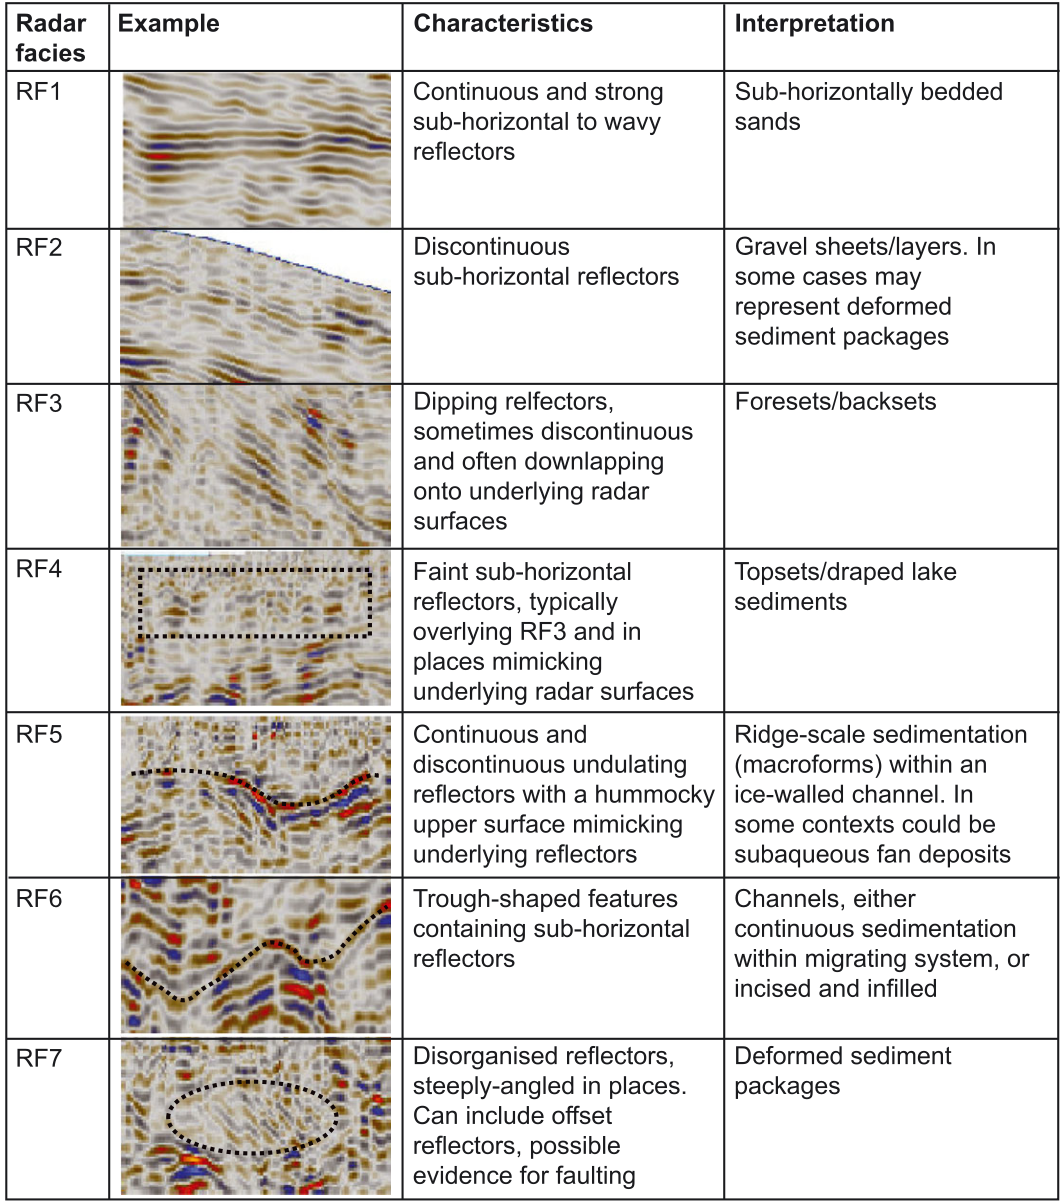
\includegraphics[width=0.9\linewidth]{Figures/0.2GPR/Lovell_2019_1.png}
    \caption[Kame belt morphology (1).]{Kame belt morphology (1). \textbf{Keywords: } Continuous, sub-horizontal, wavy, discontinuous, dipping, downlap, undulating, hummocky, chaotic \citep{Lovell2019}.}
    \label{fig:Lovell2019-1}
\end{figure}
\clearpage
\begin{figure}[h!]
    \centering
    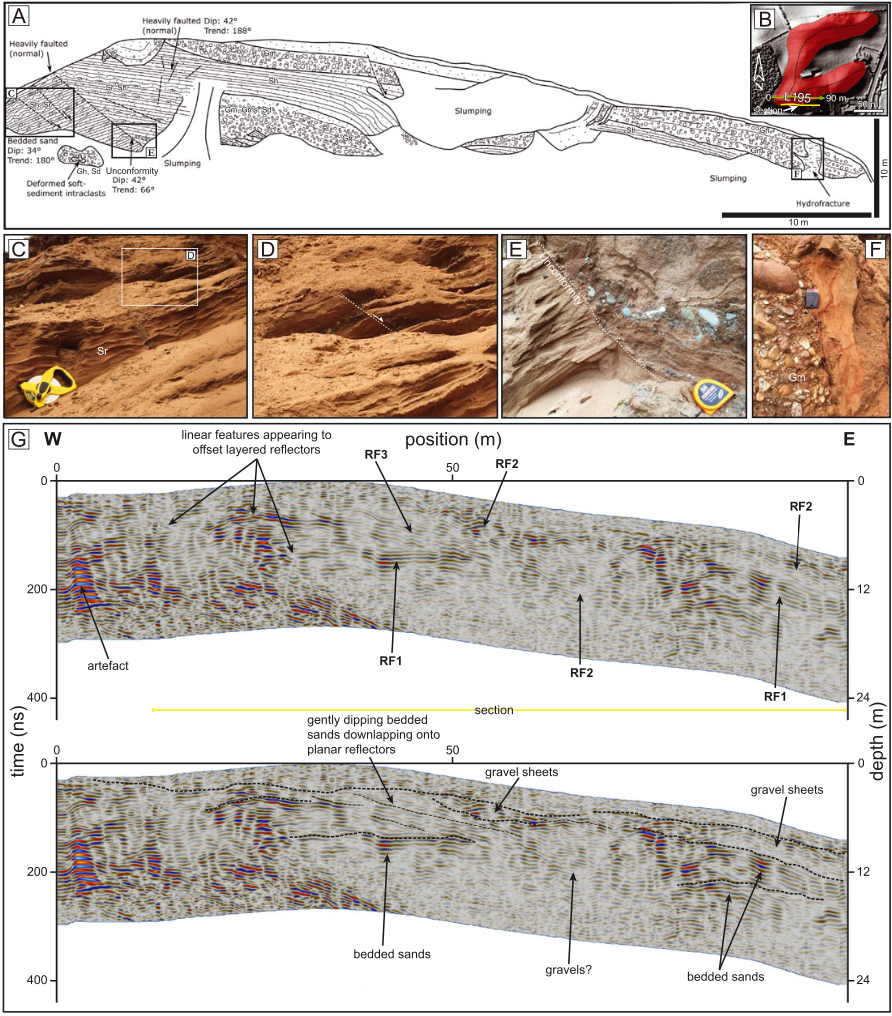
\includegraphics[width=0.9\linewidth]{Figures/0.2GPR/Lovell_2019_3.png}
    \caption[Kame belt morphology (2).]{Kame belt morphology (2). \textbf{Keywords: } Varied reflectivity, discontinuous, downlap, dipping, semi-horizontal \citep{Lovell2019}.}
    \label{fig:Lovell2019-3}
\end{figure}
\clearpage

\begin{figure}[h!]
    \centering
    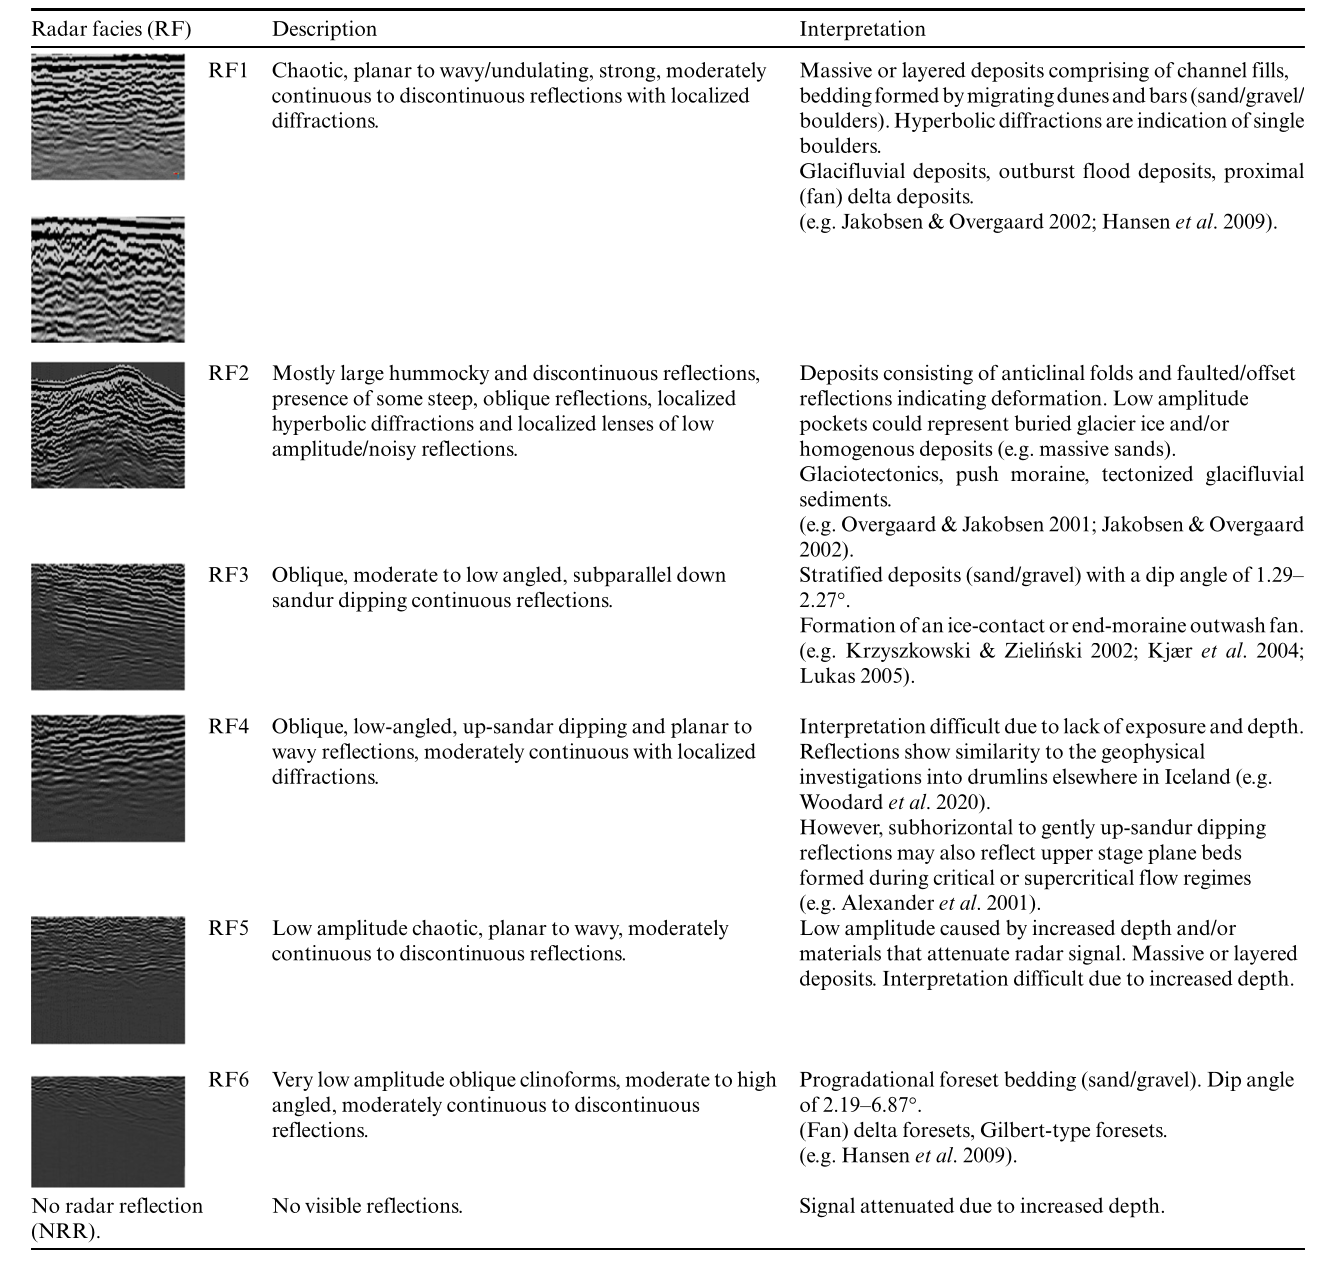
\includegraphics[width=0.9\linewidth]{Figures/0.2GPR/Harrison2022_IceMargin.png}
    \caption[Buried ice-marginal landsystem.]{Buried ice-marginal landsystem. \textbf{Keywords: } Chaotic, planar, wavy, undulating, strong, continuous, discontinuous, diffraction, hummocky, steep, oblique, hyperbolic, noisy, low amplitude, low angled, subparallel, dipping \citep{Harrison2022}.}
    \label{fig:Harrison2022-1}
\end{figure}


\begin{figure}[h!]
    \centering
    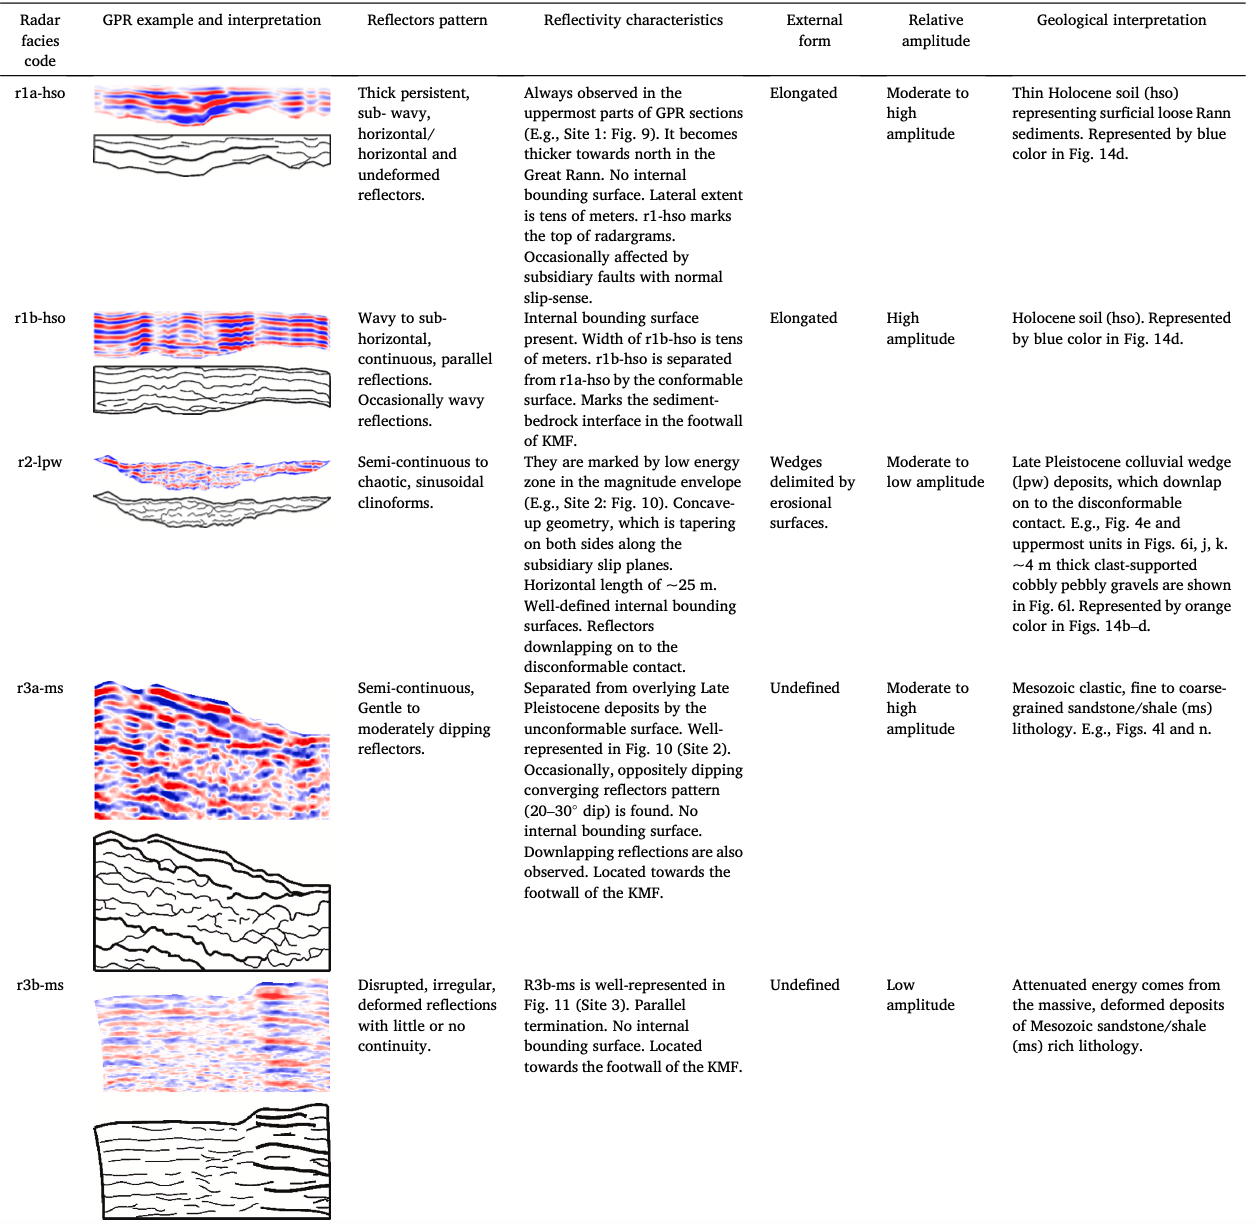
\includegraphics[width=0.9\linewidth]{Figures/0.2GPR/Shaikh2022_fault_1.png}
    \caption[Active fault zone deposits.]{Active fault zone deposits. \textbf{Keywords: } Disrupted, irregular, deformed, low continuity, parallel, low amplitude, semi-continuous, dipping, moderate amplitude, high amplitude \citep{Shaikh2022}.}
    \label{fig:Shaikh2022-1}
\end{figure}

\begin{landscape}
\begin{figure}[h!]
    \centering
    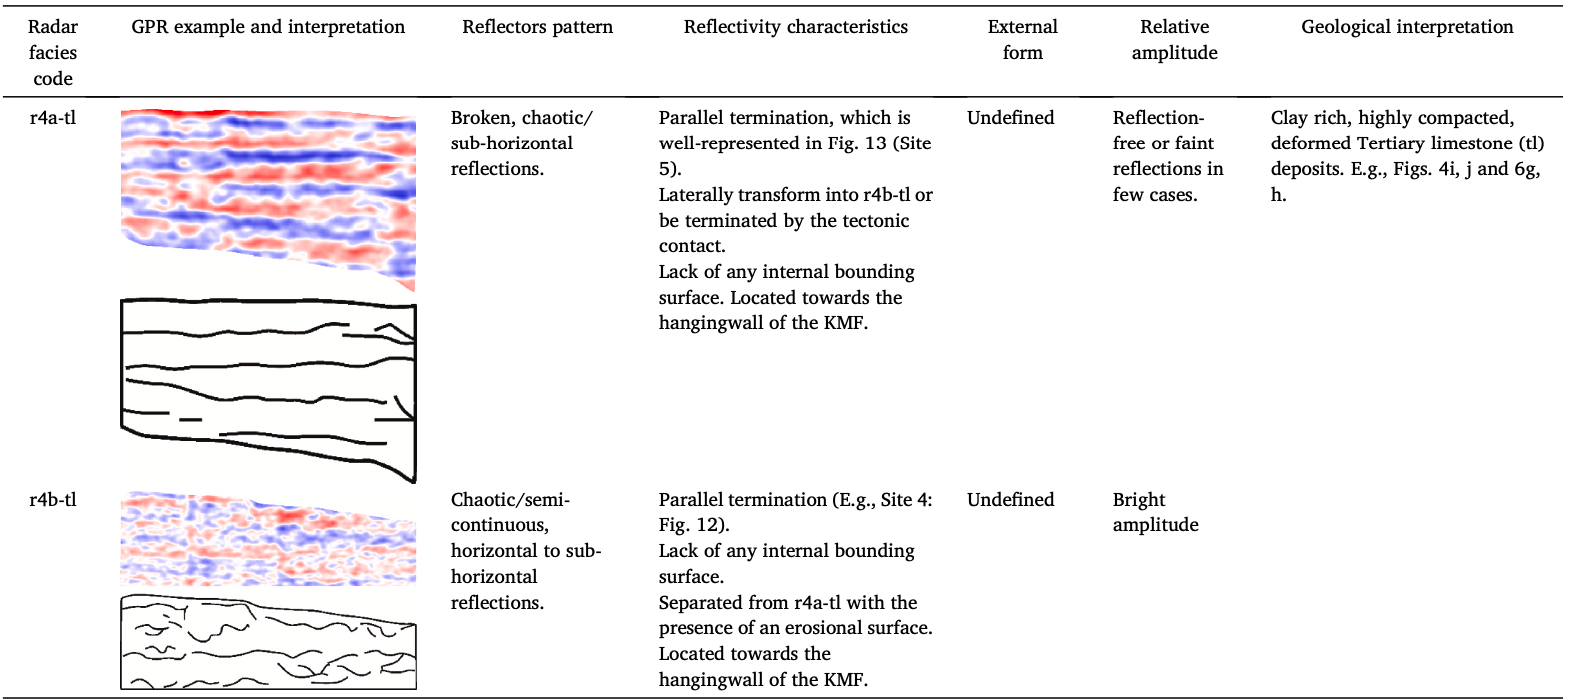
\includegraphics[width=0.9\linewidth]{Figures/0.2GPR/Shaikh2022_fault_2.png}
    \caption[Active fault deposits.]{Active fault deposits. \textbf{Keywords: } Discontinuous, chaotic, sub-horizontal, semi-continuous, horizontal, parallel, high amplitude \citep{Shaikh2022}.}
    \label{fig:Shaikh2022-2}
\end{figure}
\end{landscape}
\clearpage

\begin{figure}[h!]
    \centering
    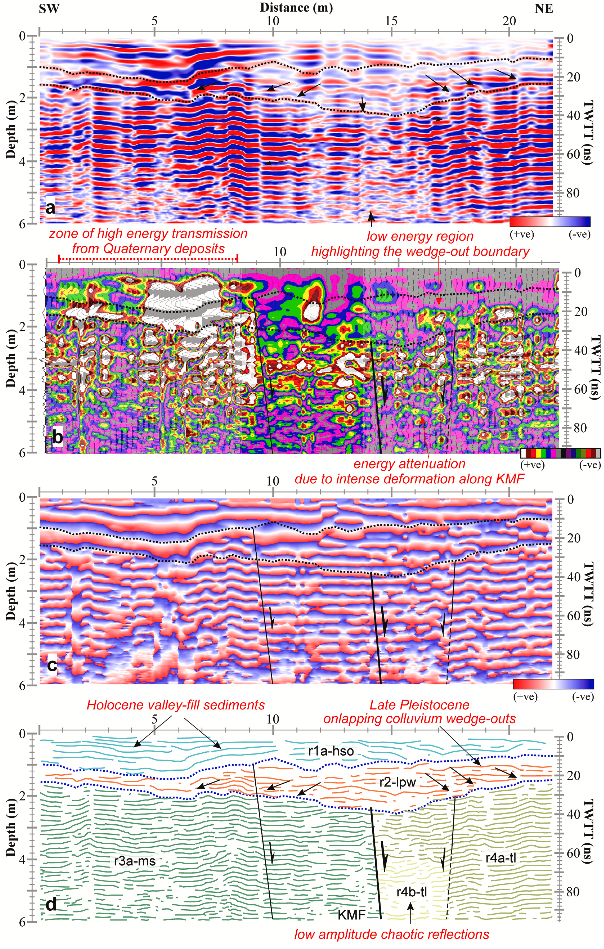
\includegraphics[width=0.9\linewidth]{Figures/0.2GPR/Shaikh2022_fault_3.png}
    \caption[Active fault deposits.]{Active fault deposits. \textbf{Keywords: } Faulting, onlap, high attenuation, discontinuity, continuous \citep{Shaikh2022}.}
    \label{fig:Shaikh2022-3}
\end{figure}

\clearpage
\subsubsection{Fluvial}
\begin{table}[h!]
\centering
\caption{Categorised GPR profile keywords for fluvial environments. Geometry, reflectivity and continuity are shown in separate columns.}
\begin{tabular}{|p{5cm}|p{5cm}|p{5cm}|}
\hline
\textbf{Geometry / Structure} & \textbf{Continuity} & \textbf{Amplitude / Reflectivity} \\
\hline
Dipping & Continuous & Low amplitude \\
Horizontal & Semi-continuous & High amplitude \\
Planar & Discontinuous & Medium amplitude \\
Parallel & & Varied reflectivity \\
Concave & & High reflectivity \\
Undulated & & Medium reflectivity \\
Onlap & & low amplitude \\
Toplap & & varied amplitude \\
Sub-horizontal & & continuous \\
Truncation & & \\
Prograding & & \\
Accretionary & & \\
Mounded & & \\
Oblique & & \\
Sigmoidal & & \\
Erosion & & \\
Truncating & & \\
Lenticular & & \\
Multidirectional dipping & & \\
Convex & & \\
Subparallel & & \\
Chaotic & & \\
Cross-bedding & & \\
Faulting & & \\
Crossing reflectors & & \\
Stratification & & \\
\hline
\end{tabular}
\label{tab:fluvial-keywords}
\end{table}

\begin{figure}[h!]
    \centering
    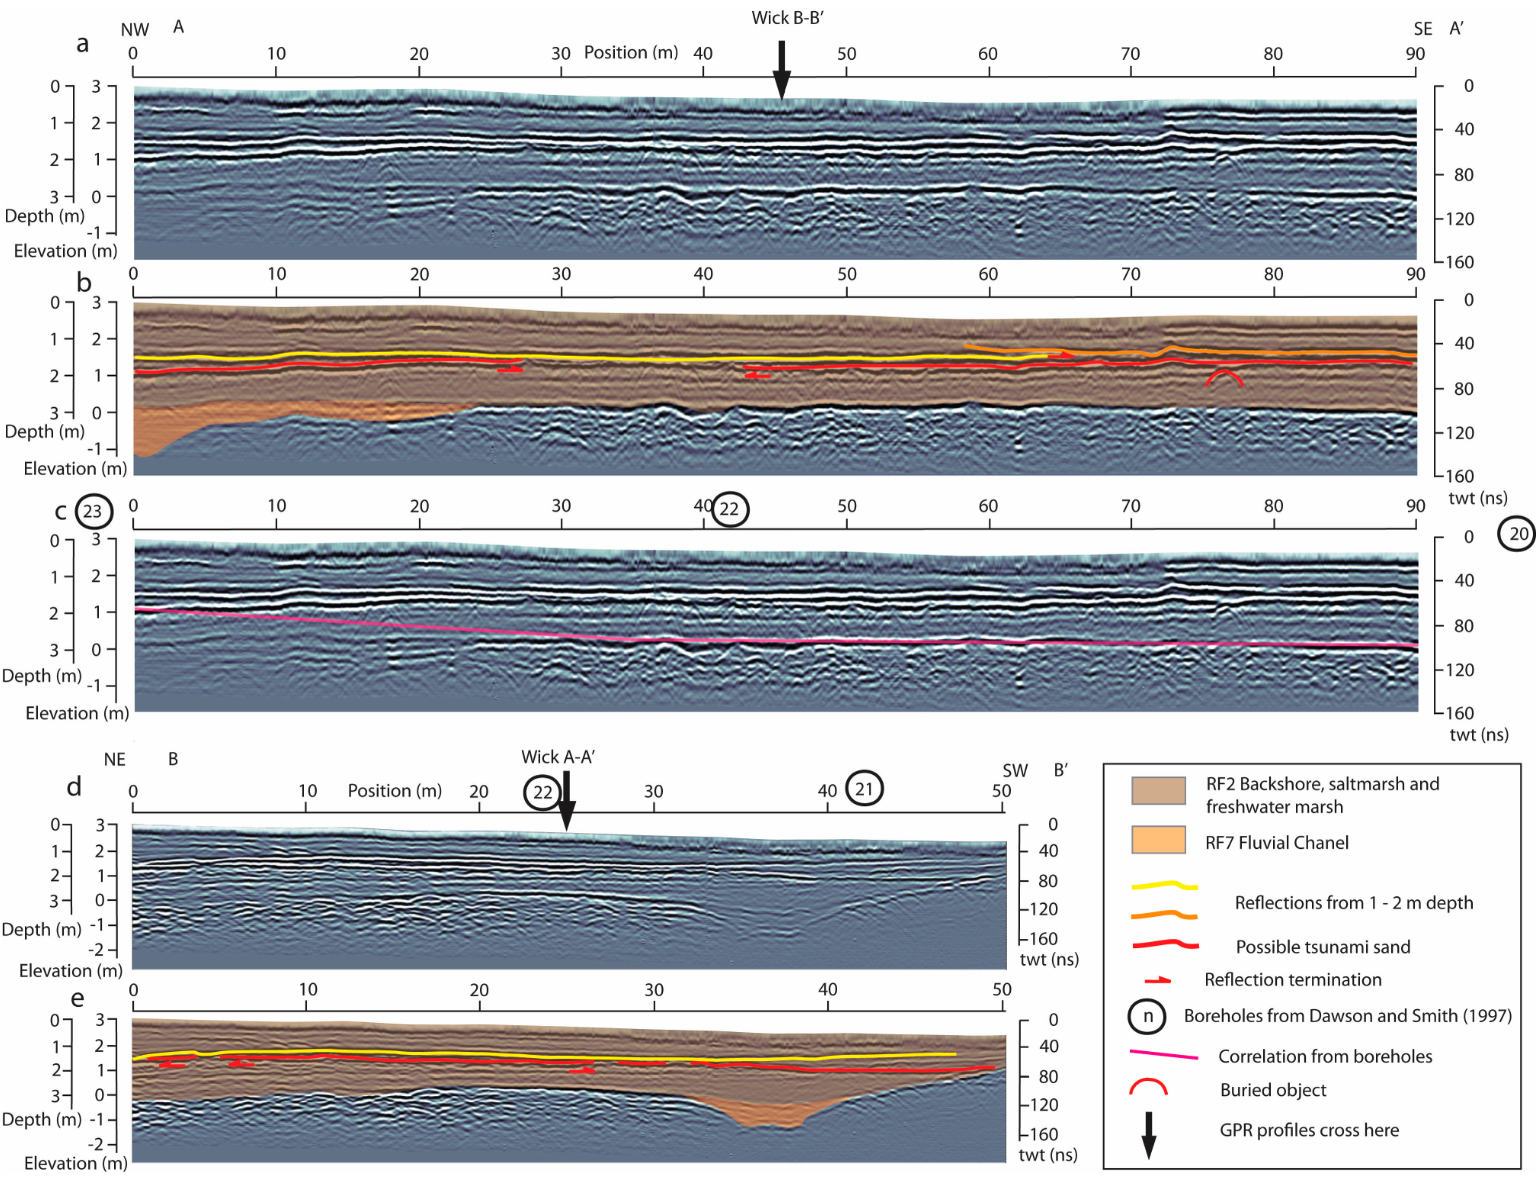
\includegraphics[width=0.9\linewidth]{Figures/0.2GPR/Bristow_2024_1.png}
    \caption[Tsunami sand.]{Tsunami sand.\textbf{Keywords: } Discontinuous, truncation, subparallel \citep{Bristow2024}.}
    \label{fig:Bristow2024-1}
\end{figure}

\begin{figure}[h!]
    \centering
    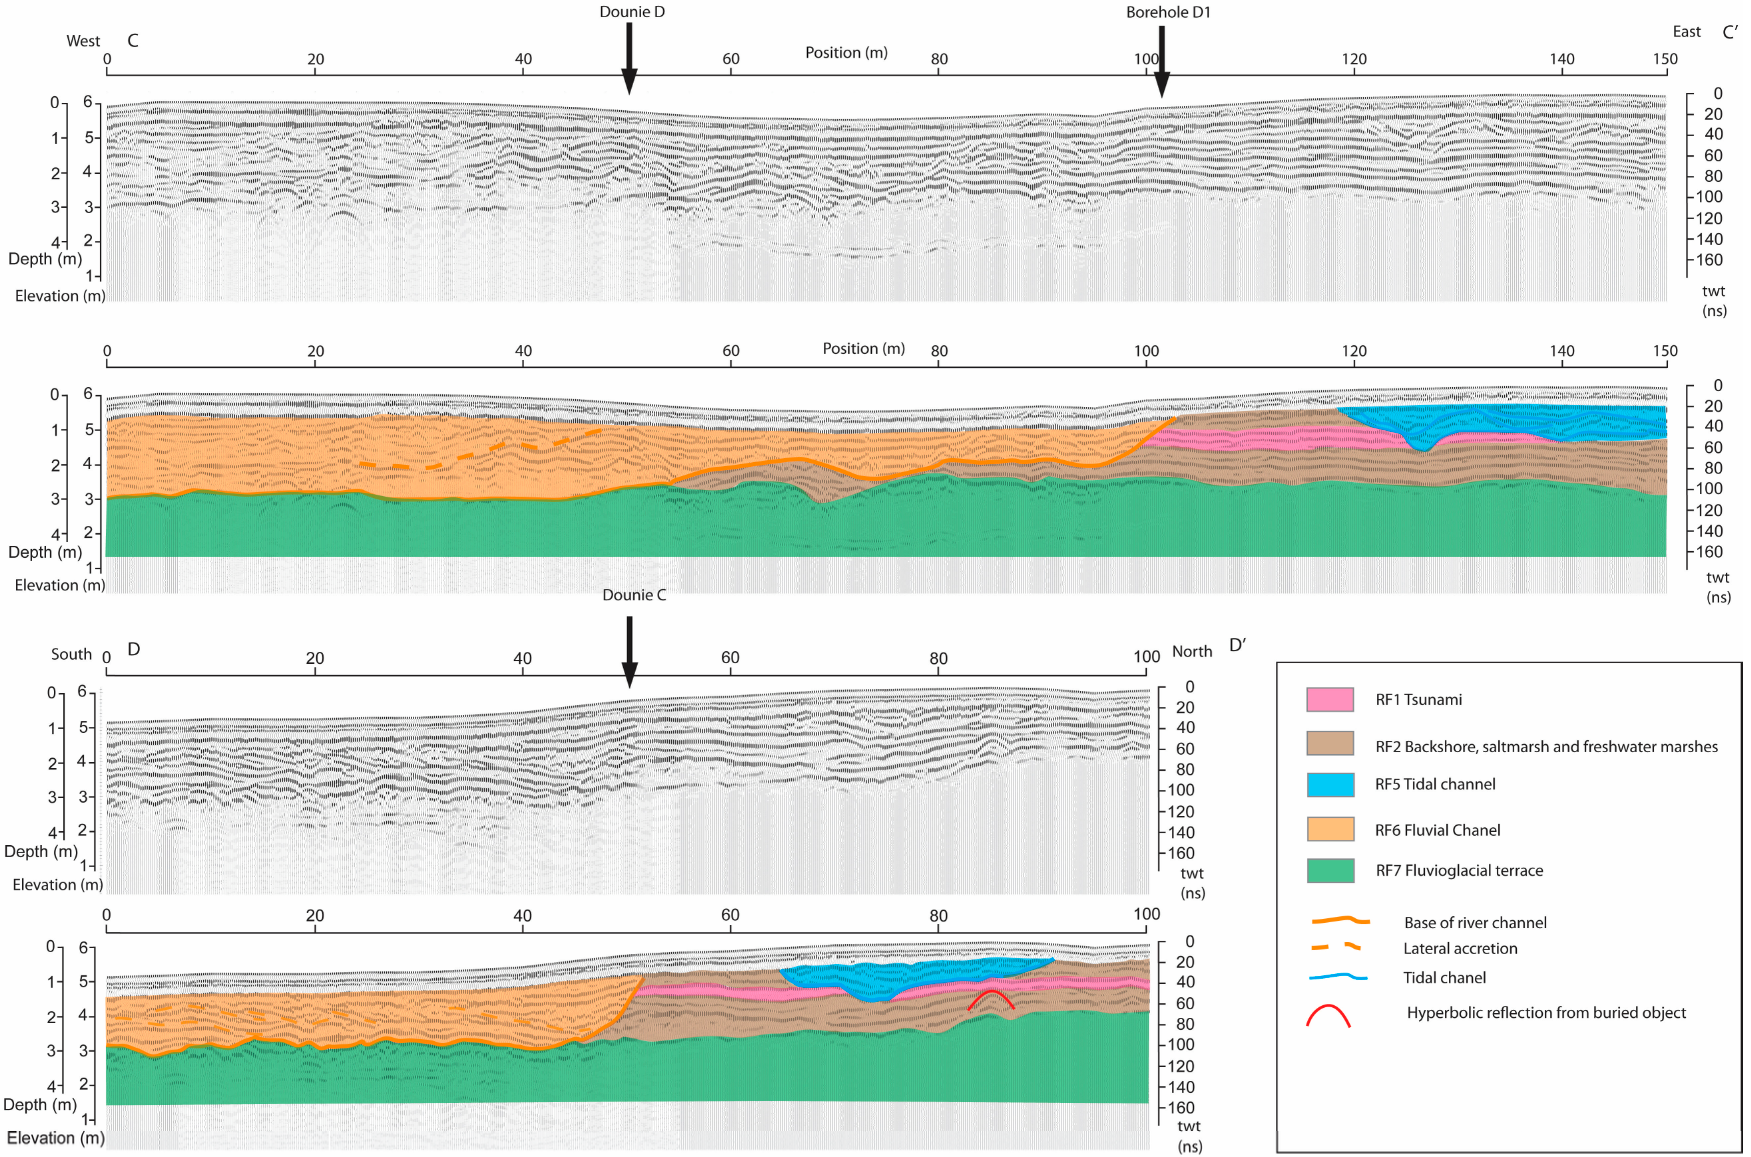
\includegraphics[width=0.9\linewidth]{Figures/0.2GPR/Bristow_2024_5.png}
    \caption[River deposits cutting into tsunami and tidal flat sediments.]{River deposits cutting into tsunami and tidal flat sediments. \textbf{Keywords: } Low amplitude, continuous, varying amplitude, high amplitude, truncating, concave, discontinuous, sub-horizontal, dipping  \citep{Bristow2024}.}
    \label{fig:Bristow2024-5}
\end{figure}

\begin{figure}[h!]
    \centering
    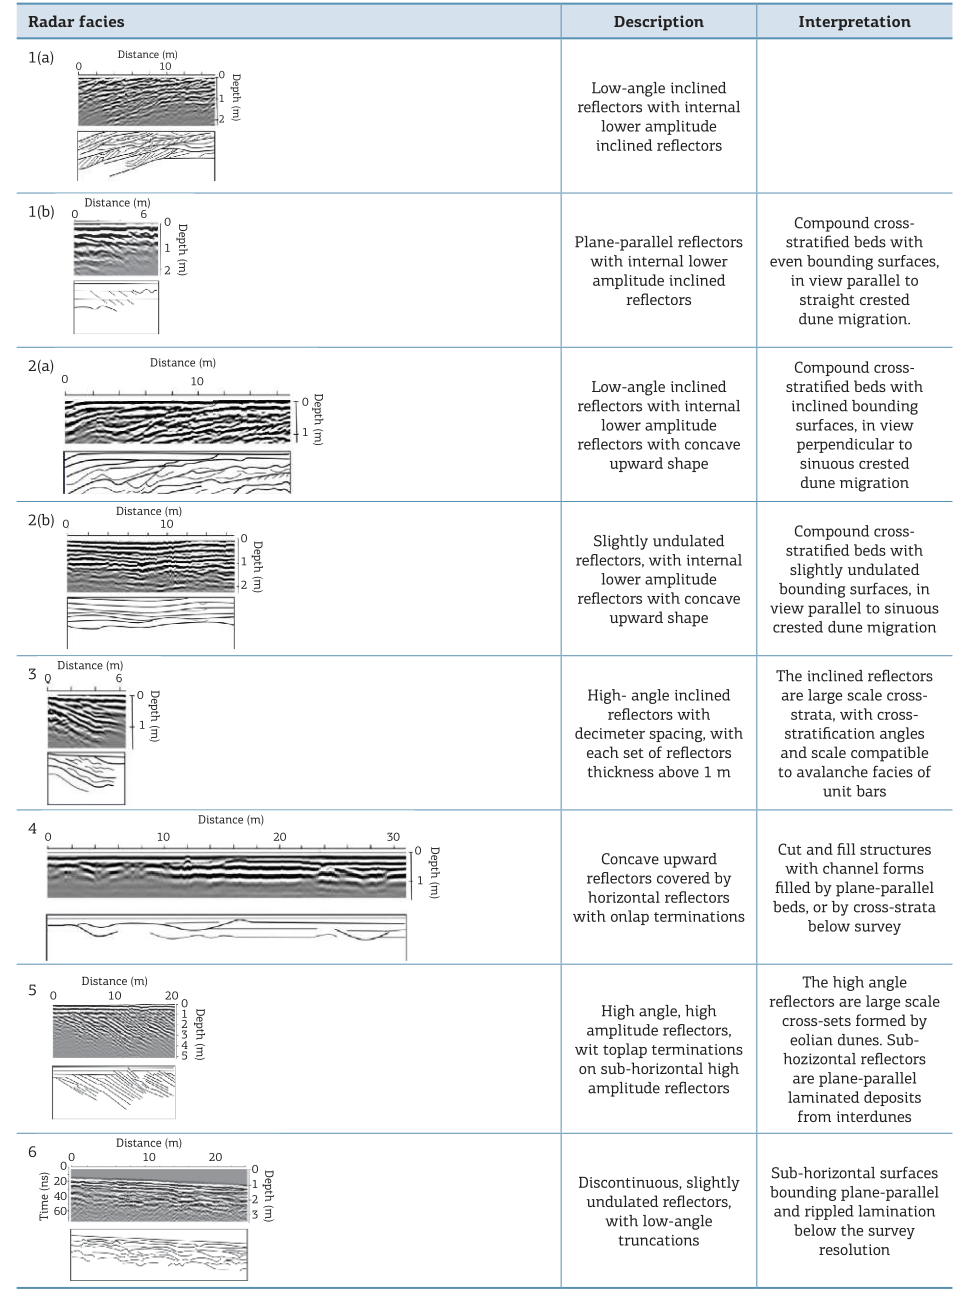
\includegraphics[width=0.9\linewidth]{Figures/0.2GPR/Tamura2016_Fluvial.png}
    \caption[Architectural elements in sedimentary structures.]{Architectural elements in sedimentary structures. \textbf{Keywords: } Dipping, inclined, low amplitude, planar, parallel, concave, undulated, high-angle, horizontal, onlap, high amplitude, toplap, sub-horizontal, discontinuous, truncation \citep{Tamura2016}.}
    \label{fig:Tamura2016-1}
\end{figure}

\begin{figure}[h!]
    \centering
    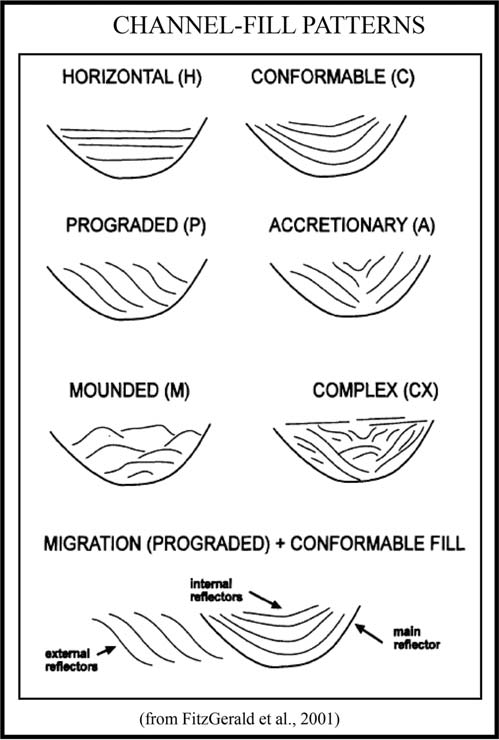
\includegraphics[width=0.9\linewidth]{Figures/0.2GPR/Maio2015_channelfill.png}
    \caption[Storm-Driven Breaching along a Transgressing Barrier System (1).]{Storm-Driven Breaching along a Transgressing Barrier System (1). \textbf{Keywords: } Horizontal, prograding, accretionary, mounded, continuous, semi-continuous, varied reflectivity, onlap, truncating   \citep{Maio2016}.}
    \label{fig:Maio2016-1}
\end{figure}

\begin{figure}[h!]
    \centering
    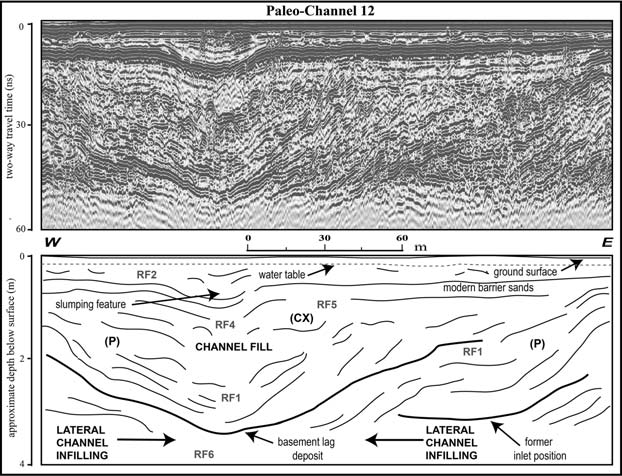
\includegraphics[width=0.9\linewidth]{Figures/0.2GPR/Maio2015_channelfill_2.png}
    \caption[Storm-Driven Breaching along a Transgressing Barrier System (2).]{Storm-Driven Breaching along a Transgressing Barrier System (2).\textbf{Keywords: } Concave, oblique, sigmoidal, discontinuous, semi-continuous, chaotic, varied amplitude, high reflectivity, truncation, erosion, onlap \citep{Maio2016}.}
    \label{fig:Maio2016-2}
\end{figure}


\begin{figure}[h!]
    \centering
    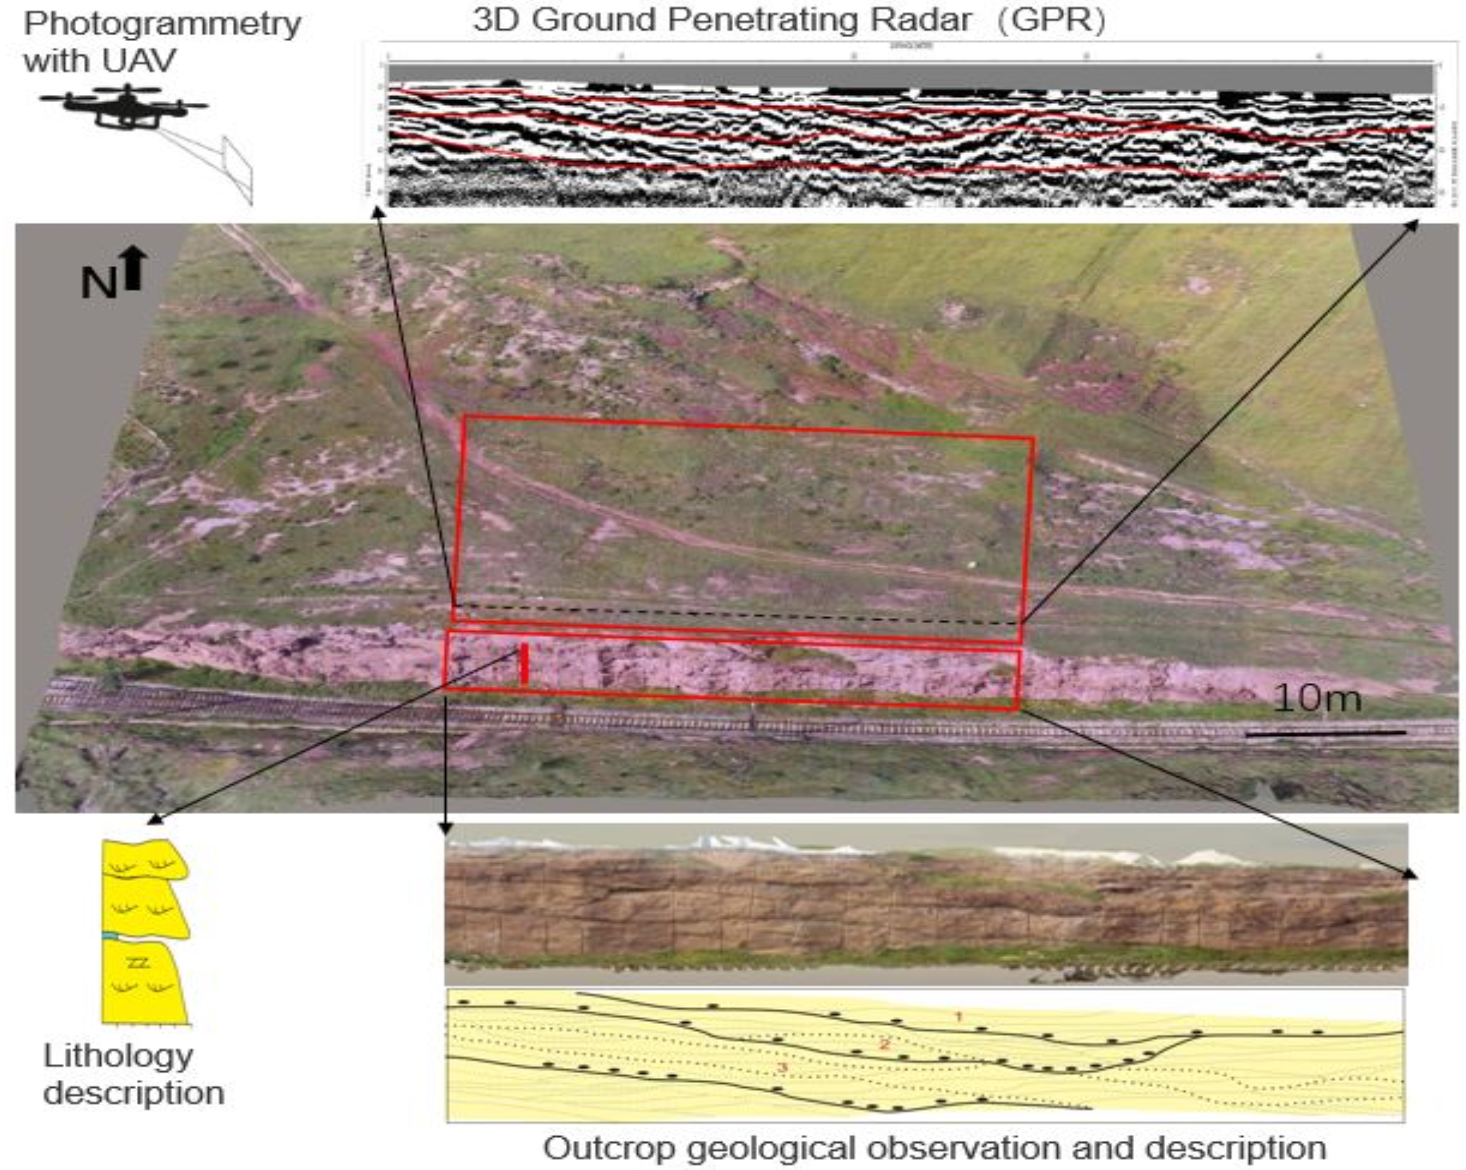
\includegraphics[width=0.9\linewidth]{Figures/0.2GPR/Guo2022_1.png}
    \caption[Sandy Braided River (1).]{Sandy Braided River (1). \textbf{Keywords: } Dipping, continuous, semi-continuous, parallel, concave, lenticular, high reflectivity \citep{Guo2022}.}
    \label{fig:Guo2022-1}
\end{figure}


\begin{figure}[h!]
    \centering
    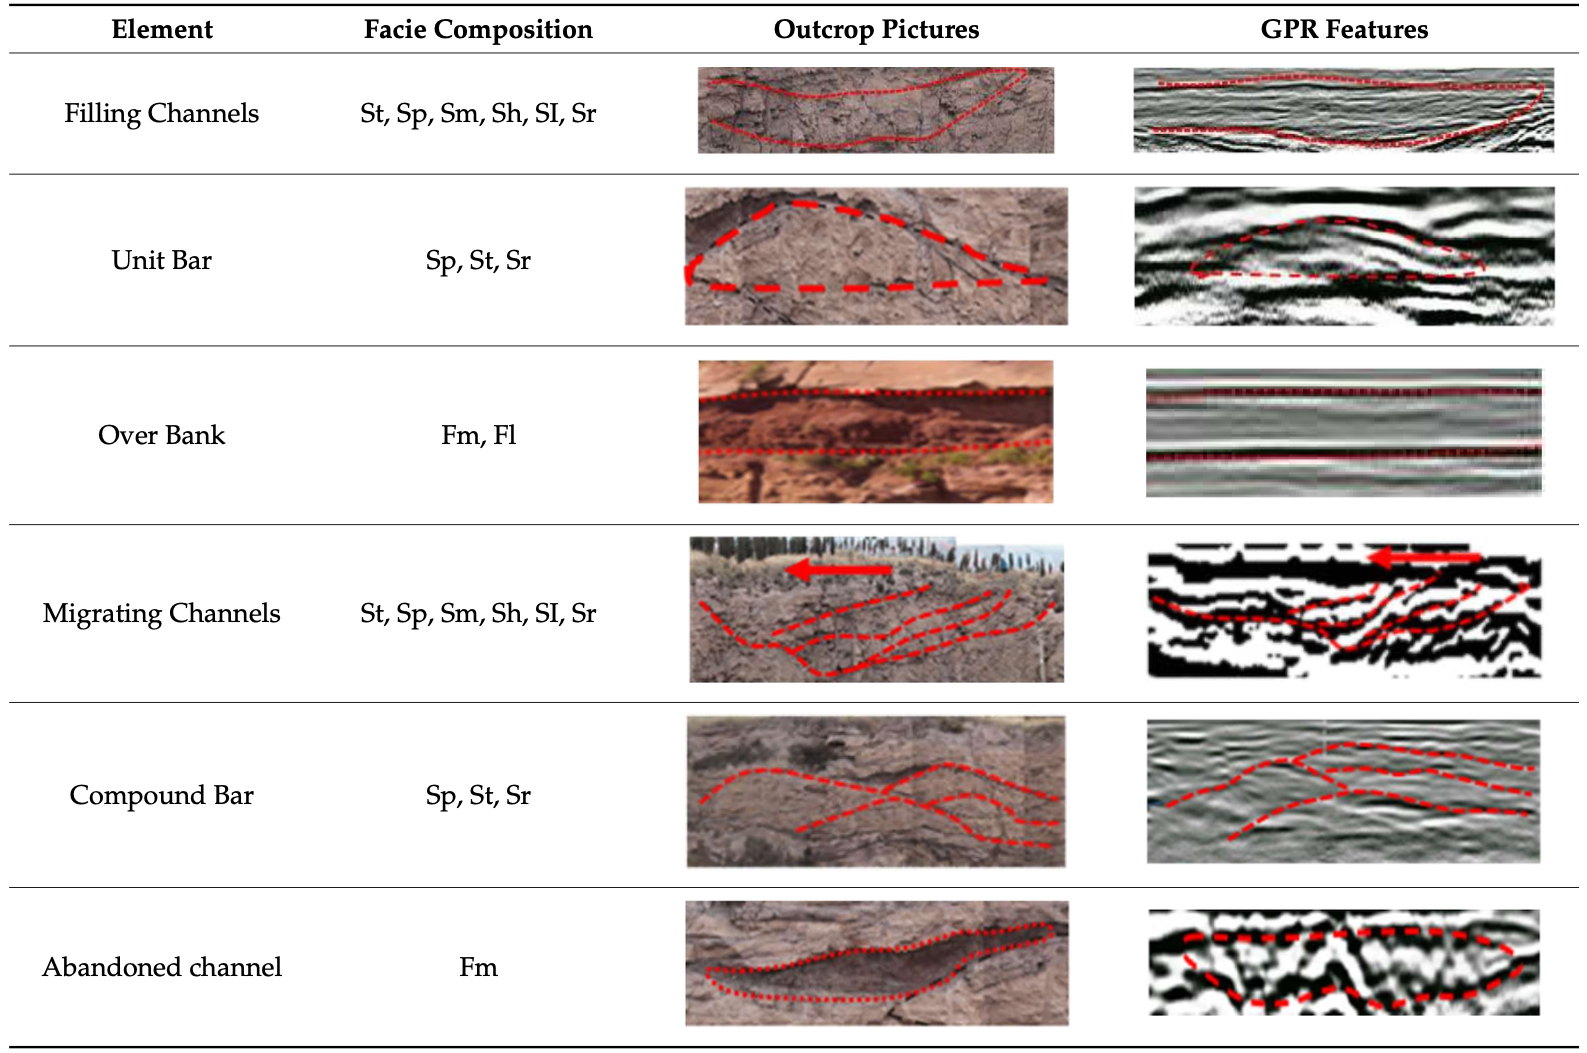
\includegraphics[width=0.9\linewidth]{Figures/0.2GPR/Guo2022_6.png}
    \caption[Sandy Braided River (2).]{Sandy Braided River (2). \textbf{Keywords: } Lenticular, multidirectional dipping, onlap, semi-horizontal, hummocky, concave, varied reflectivity, continuous, discontinuous \citep{Guo2022}.}
    \label{fig:Guo2022-6}
\end{figure}

\begin{figure}[h!]
    \centering
    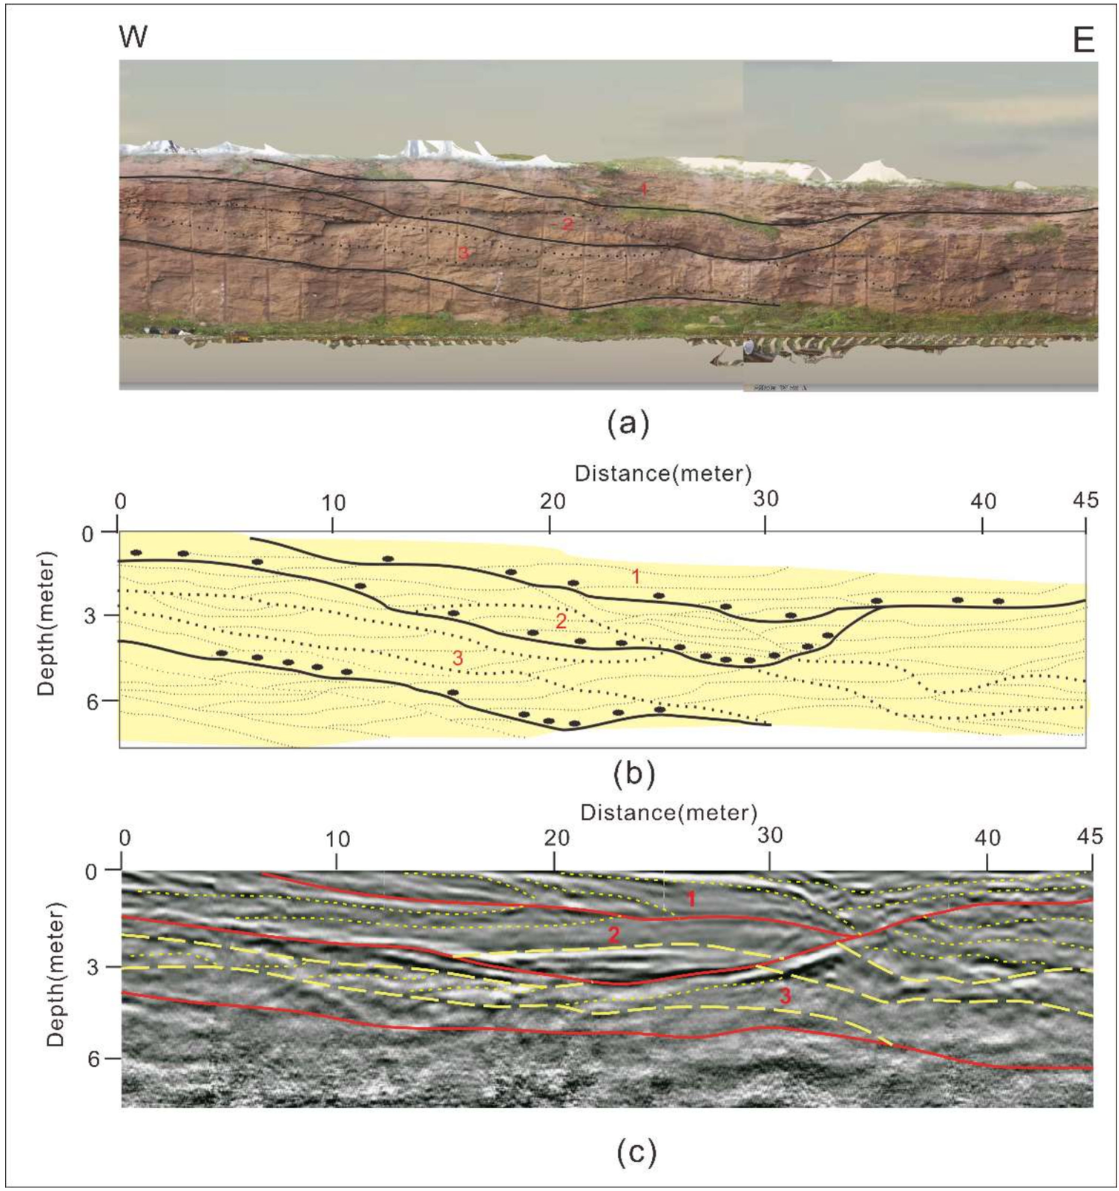
\includegraphics[width=0.9\linewidth]{Figures/0.2GPR/Guo2022_5.png}
    \caption[Sandy Braided River (3).]{Sandy Braided River (3). \textbf{Keywords:} Lenticular, horizontal, convex-down, parallel, subparallel, chaotic, low amplitude \citep{Guo2022}.}
    \label{fig:Guo2022-5}
\end{figure}


\begin{figure}[h!]
    \centering
    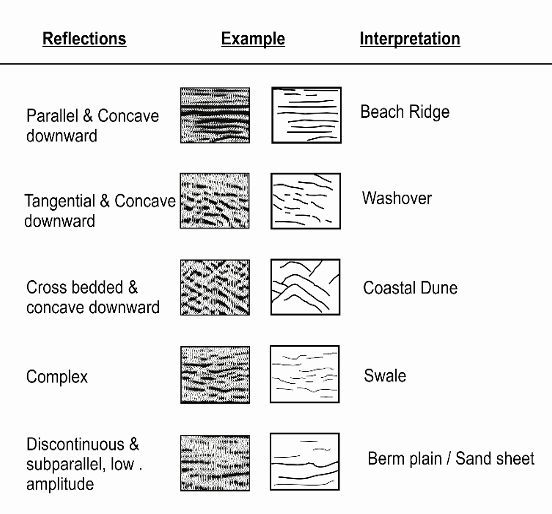
\includegraphics[width=0.9\linewidth]{Figures/0.2GPR/Shukla2013_Coastal_margin.png}
    \caption[Sedimentary architecture and coastal dynamics.]{Sedimentary architecture and coastal dynamics. \textbf{Keywords: } Parallel, concave, cross-bedding, discontinuous, subparallel, low amplitude, horizontal, dipping \citep{Shukla2013}.}
    \label{fig:Shukla2013-1}
\end{figure}

\begin{figure}[h!]
    \centering
    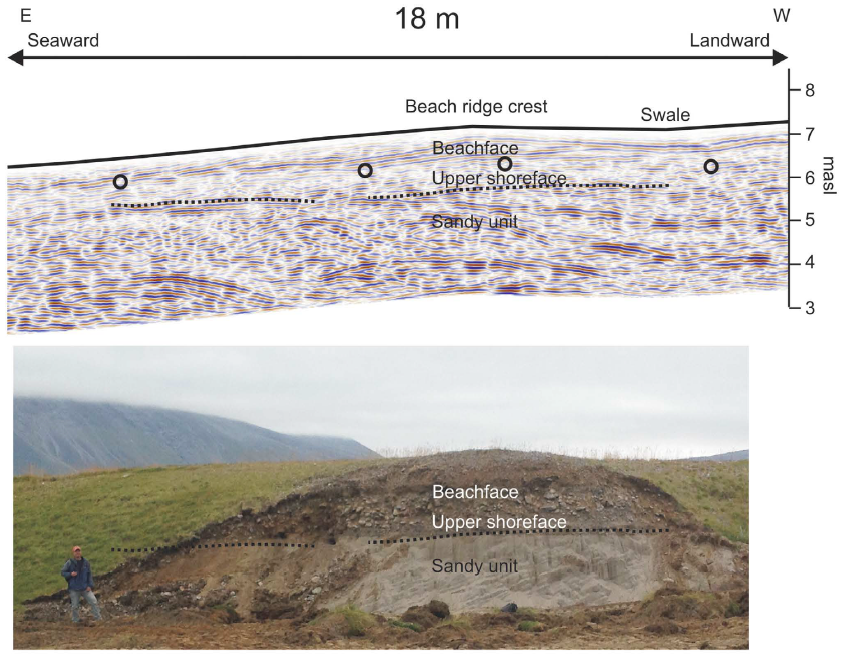
\includegraphics[width=0.9\linewidth]{Figures/0.2GPR/Nielsen_2017_beach.png}
    \caption[Beach ridge eroded by river.]{Beach ridge eroded by river. \textbf{Keywords: } Dipping, medium reflectivity, semi-continuous, hummocky, truncation, erosion, semi-horizontal \citep{Nielsen2017}.}
    \label{fig:Nielsen2017-beach-1}
\end{figure}

\begin{figure}[h!]
    \centering
    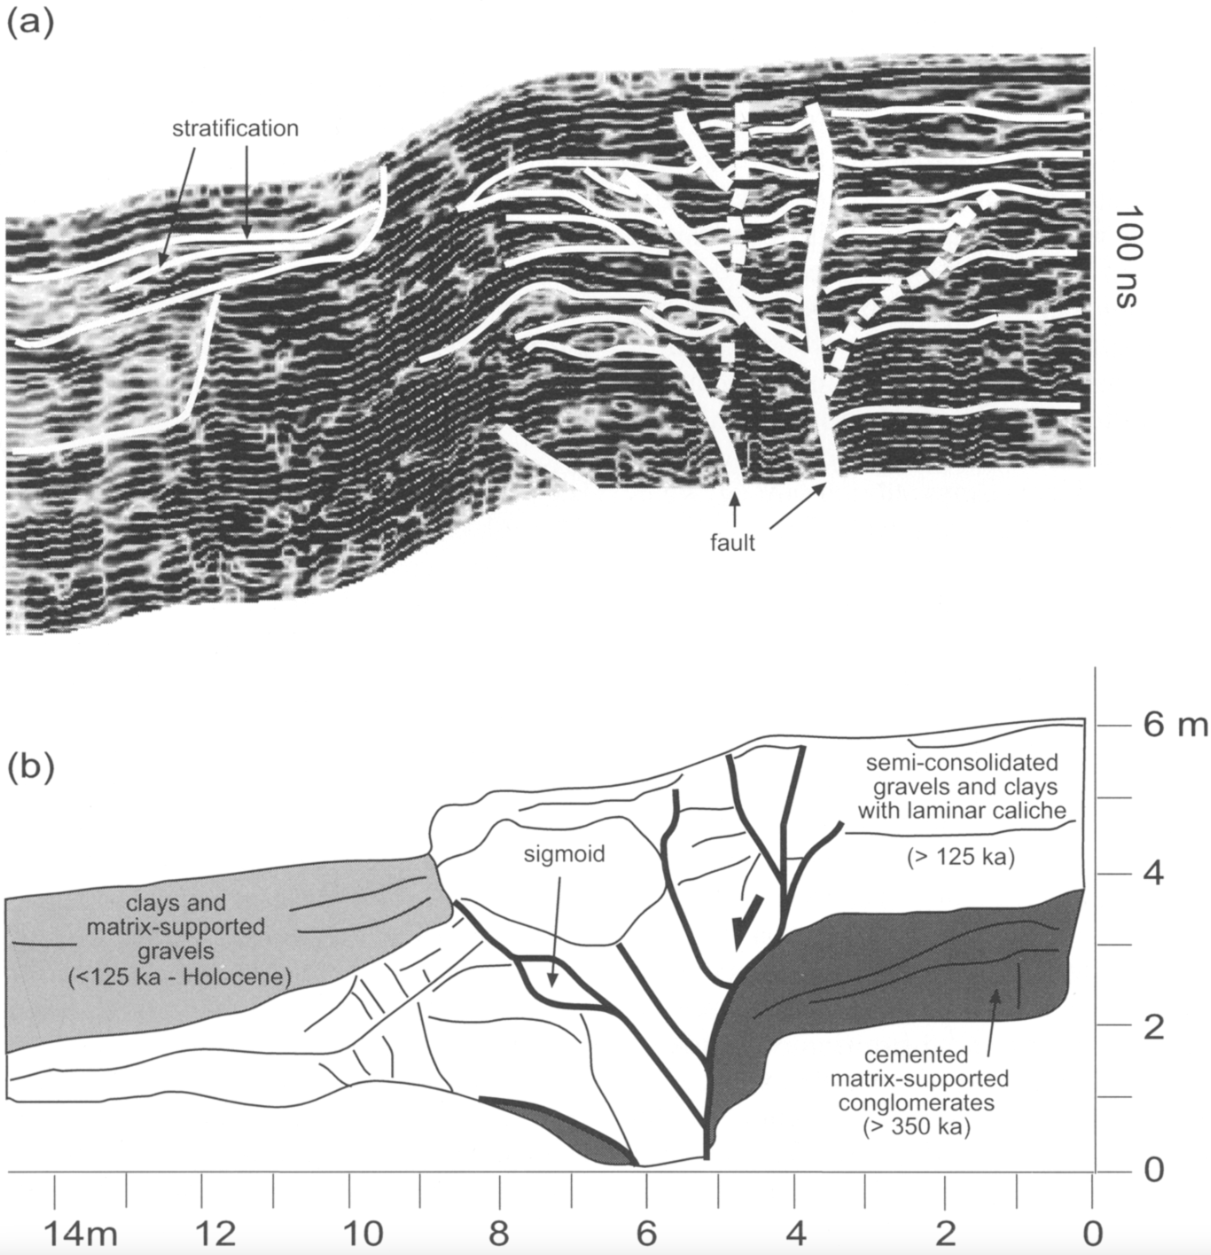
\includegraphics[width=0.9\linewidth]{Figures/0.2GPR/reiss2003_normal-faults_1.png}
    \caption[Active normal faults and associated sediments (1).]{Active normal faults and associated sediments (1).\textbf{Keywords: } Sigmoid, faulting, discontinuous, parallel, stratification, medium amplitude \citep{Reiss2003}.}
    \label{fig:Reiss2003-1}
\end{figure}

\begin{figure}[h!]
    \centering
    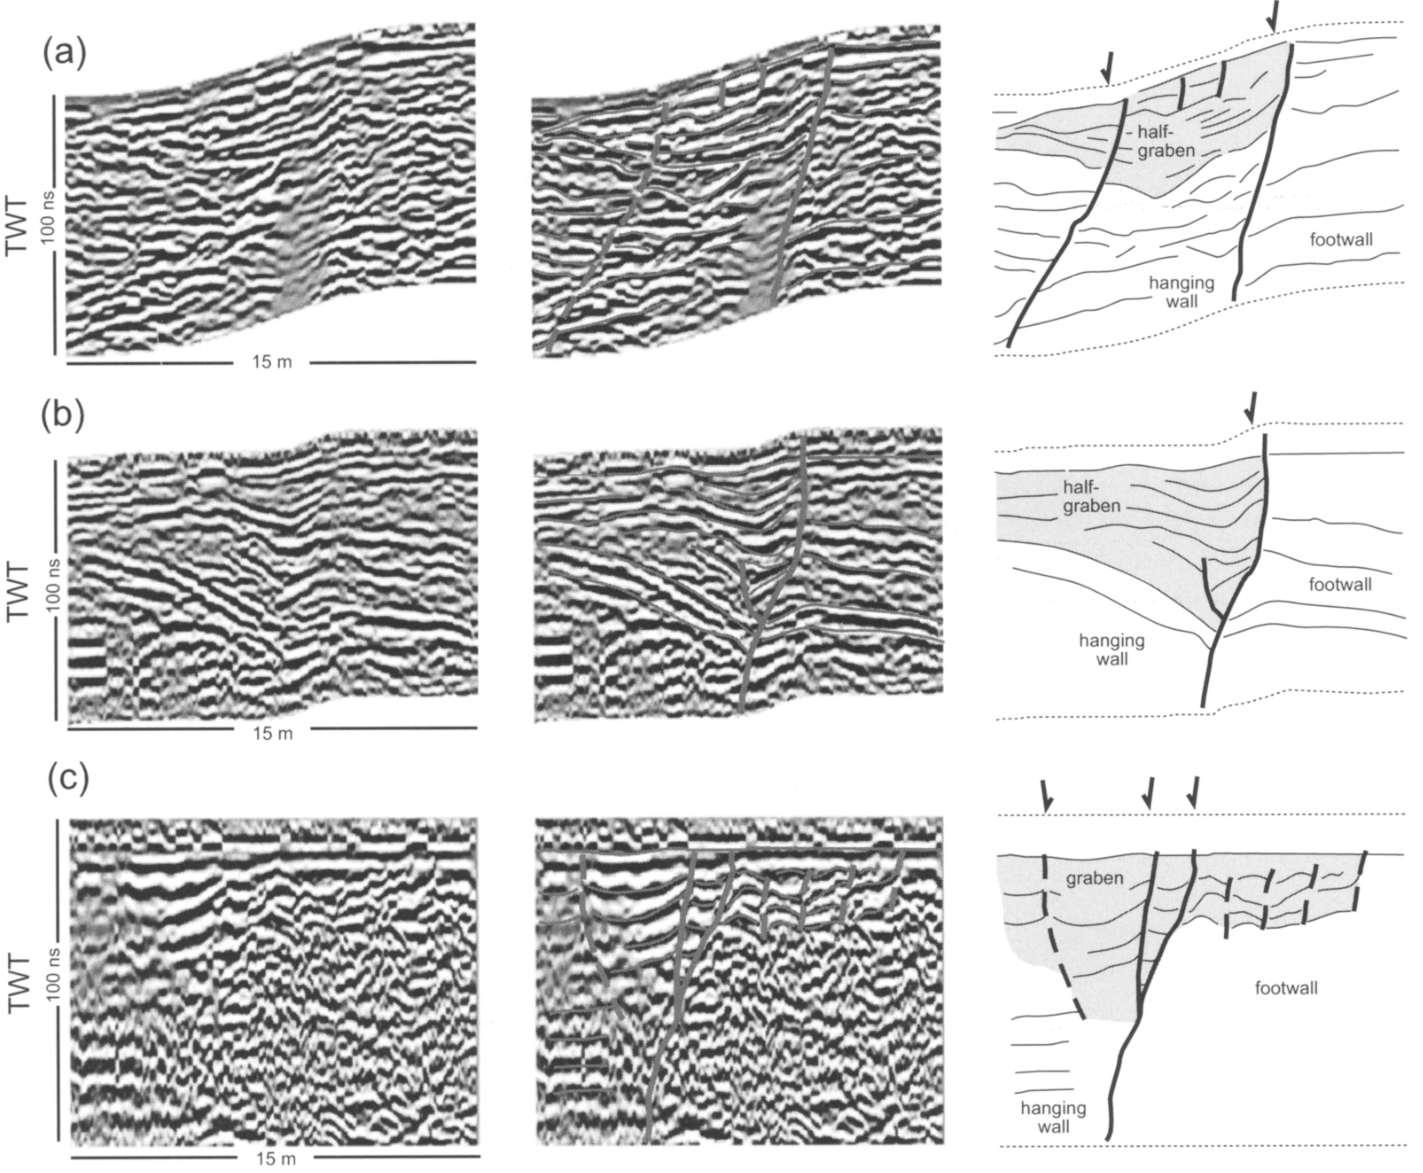
\includegraphics[width=0.9\linewidth]{Figures/0.2GPR/reiss2003_normal-faults_2.png}
    \caption[Active normal faults and associated sediments (2).]{Active normal faults and associated sediments (2). \textbf{Keywords: } Dipping, parallel, crossing reflectors, discontinuous, high amplitude \citep{Reiss2003}.}
    \label{fig:Reiss2003-2}
\end{figure}
\clearpage
\subsubsection{Deltaic}
\begin{table}[h!]
\centering
\caption{Categorised GPR profile keywords for igneous environments. Geometry, reflectivity and continuity are shown in separate columns.}
\begin{tabular}{|p{6.5cm}|p{6.5cm}|}
\hline
\textbf{Geometry / Structure} & \textbf{Continuity / Amplitude / Reflectivity} \\
\hline
Parallel & High amplitude \\
Concave & Semi-continuous \\
Tangential & Discontinuous \\
Cross-bedding & Varied amplitude \\
Complex & High reflectivity \\
Subparallel & Low reflectivity \\
Multidirectional dipping & Varied reflectivity \\
Subhorizontal/Semi-horizontal & Low attenuation \\
Horizontal & High attenuation \\
Prograding & Continuous \\
Clinoform & Medium amplitude \\
Sigmoidal & Low amplitude \\
Dipping/Inclined/slight dipping & \\
Tabular & \\
Ridge & \\
Onlap & \\
Truncation & \\
Bounding surface & \\
Hyperbolic & \\
Convex/Curved& \\
Erosion / Erosional & \\
Hummocky/Sinuous & \\
Oblique & \\
Wedge & \\
Lenticular & \\
Chaotic & \\
Unconformity & \\
Undulating & \\
Toplap & \\
Semi-parallel & \\
\hline
\end{tabular}
\label{tab:coastal-keywords}
\end{table}
 
\begin{figure}[h!]
    \centering
    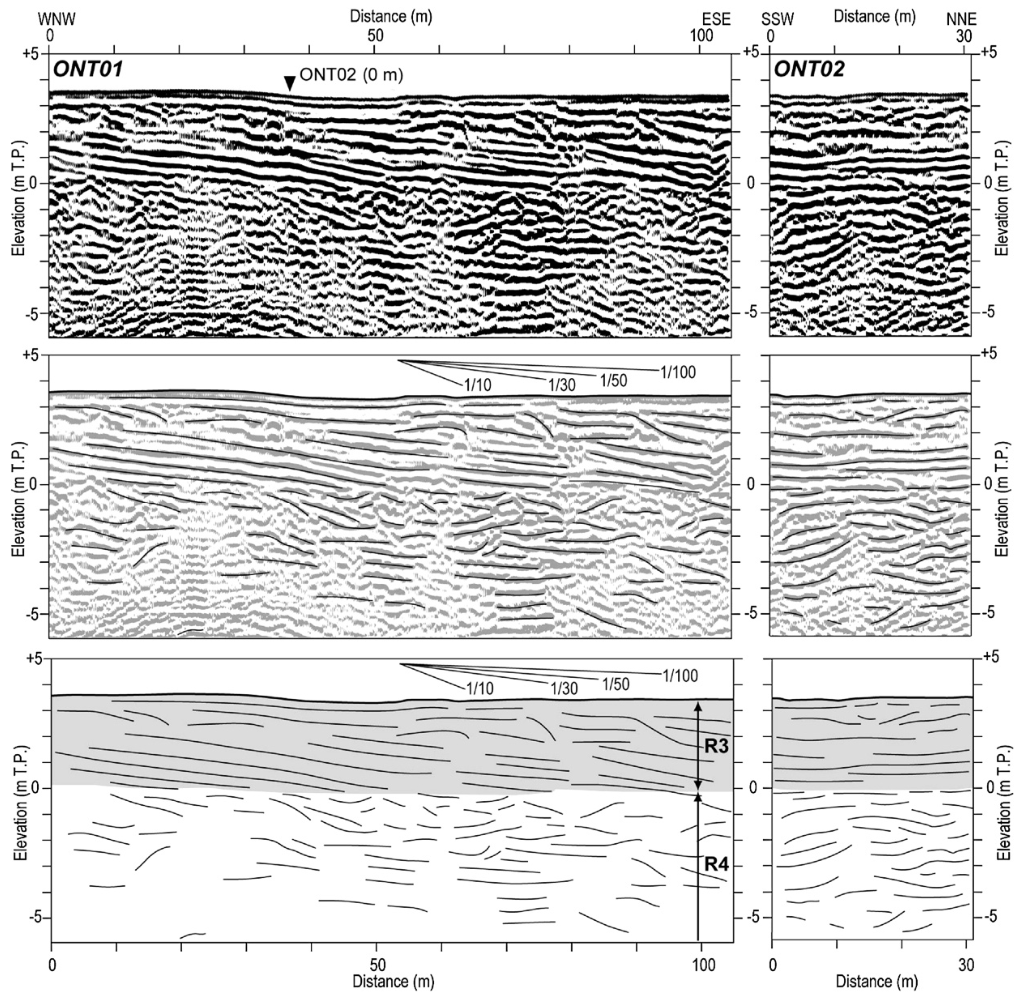
\includegraphics[width=0.9\linewidth]{Figures/0.2GPR/Tamura2008_2.png}
    \caption[Foreshore and upper shoreface deposits.]{Foreshore and upper shoreface deposits. \textbf{Keywords: } Parallel, concave, tangential, cross-bedding, complex, discontinuous, subparallel, low amplitude, multidirectional dipping  \citep{Tamura2008}.}
    \label{fig:Tamura2008-2}
\end{figure}

\begin{figure}[h!]
    \centering
    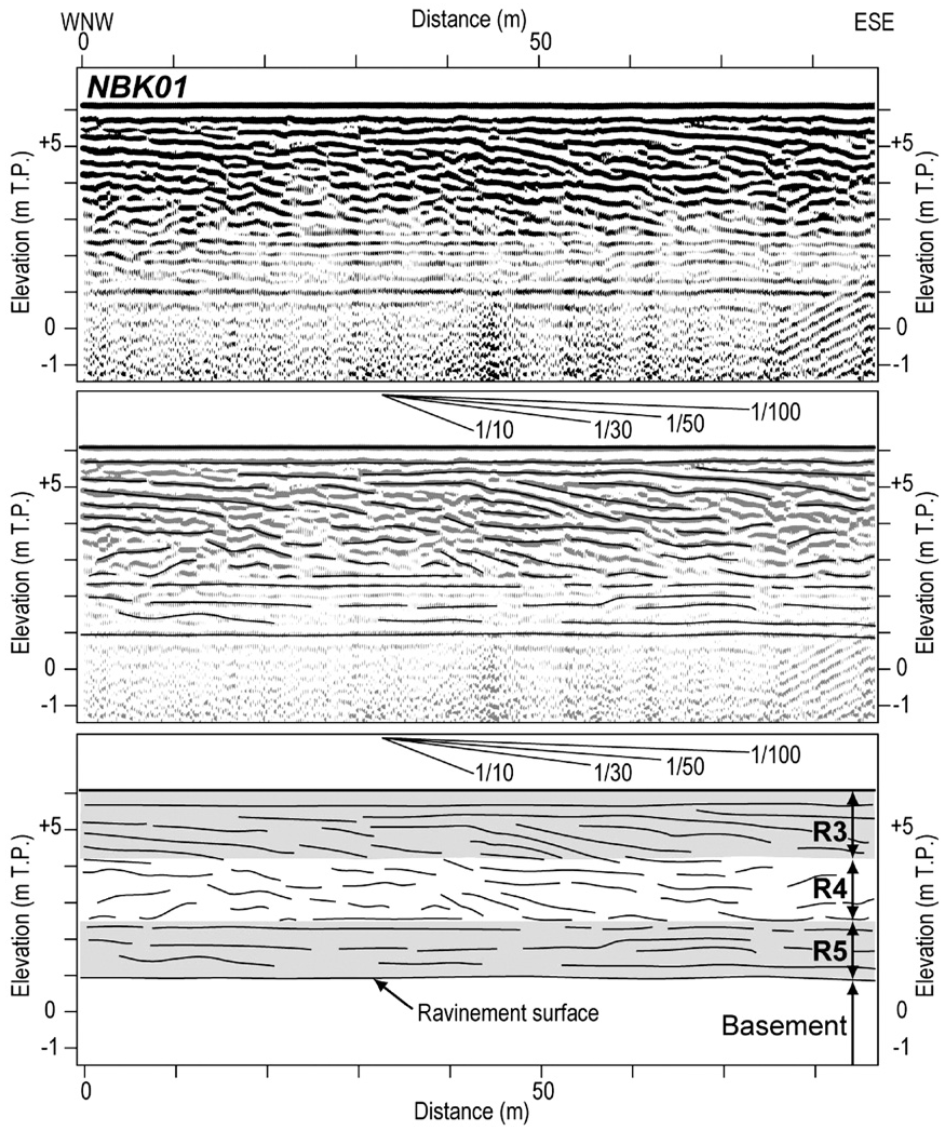
\includegraphics[width=0.9\linewidth]{Figures/0.2GPR/Tamura2008_4.png}
    \caption[Shore-normal transect (2).]{Shore-normal transect. \textbf{Keywords: } Continuous, subhorizontal, horizontal, discontinuous, multidirectional dipping, varied amplitude  \citep{Tamura2008}.}
    \label{fig:Tamura2008-4}
\end{figure}
\begin{landscape}
    \begin{figure}[h!]
    \centering
    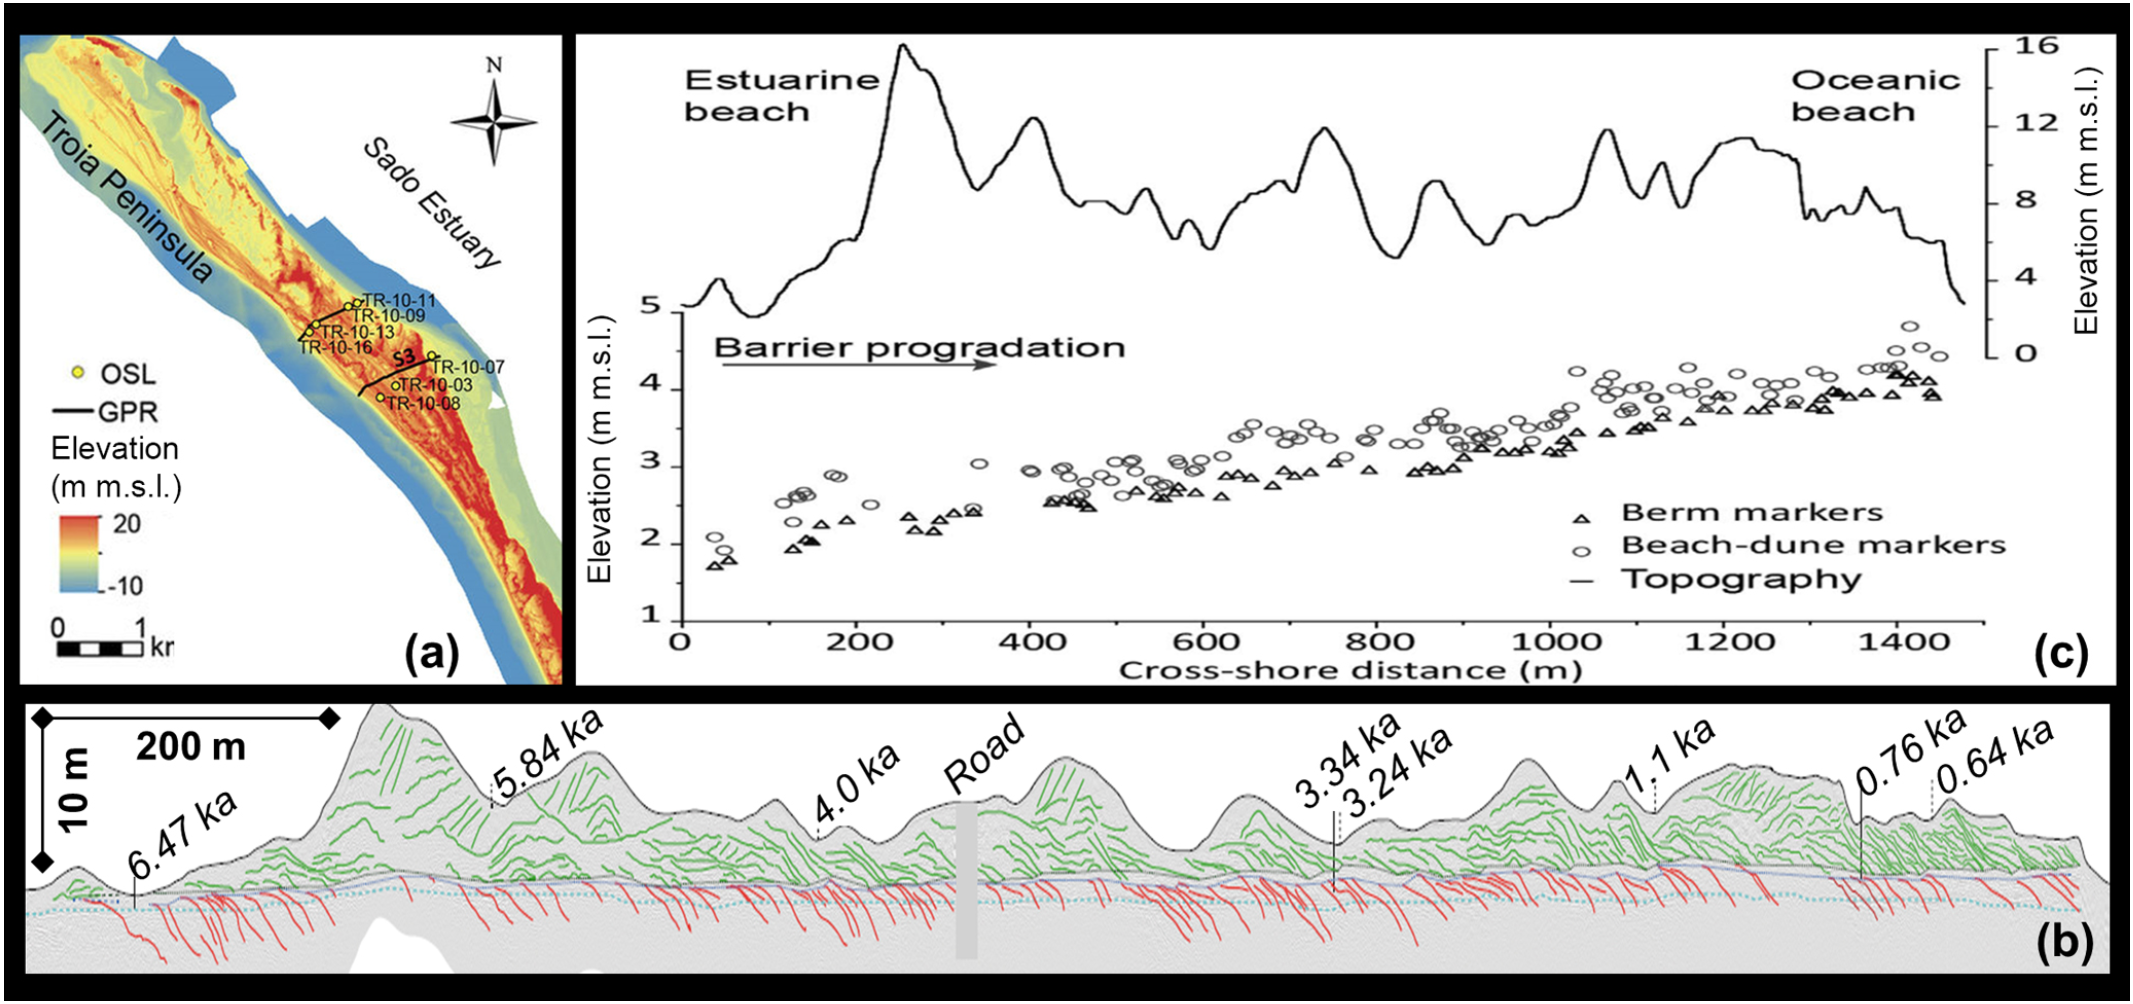
\includegraphics[width=0.9\linewidth]{Figures/0.2GPR/dougherty2019-1.png}
    \caption[Shoreline evolution (1).]{Shoreline evolution (1). \textbf{Keywords: } Prograding, clinoforms, sigmoidal, dipping, tabular, sub-horizontal, concave, downlap, ridge, continuous, semi-continuous, laterally extensive, varied amplitude, truncation, onlap \citep{Dougherty2019}.}
    \label{fig:dougherty2019-1}
\end{figure}
\end{landscape}

\begin{figure}[h!]
    \centering
    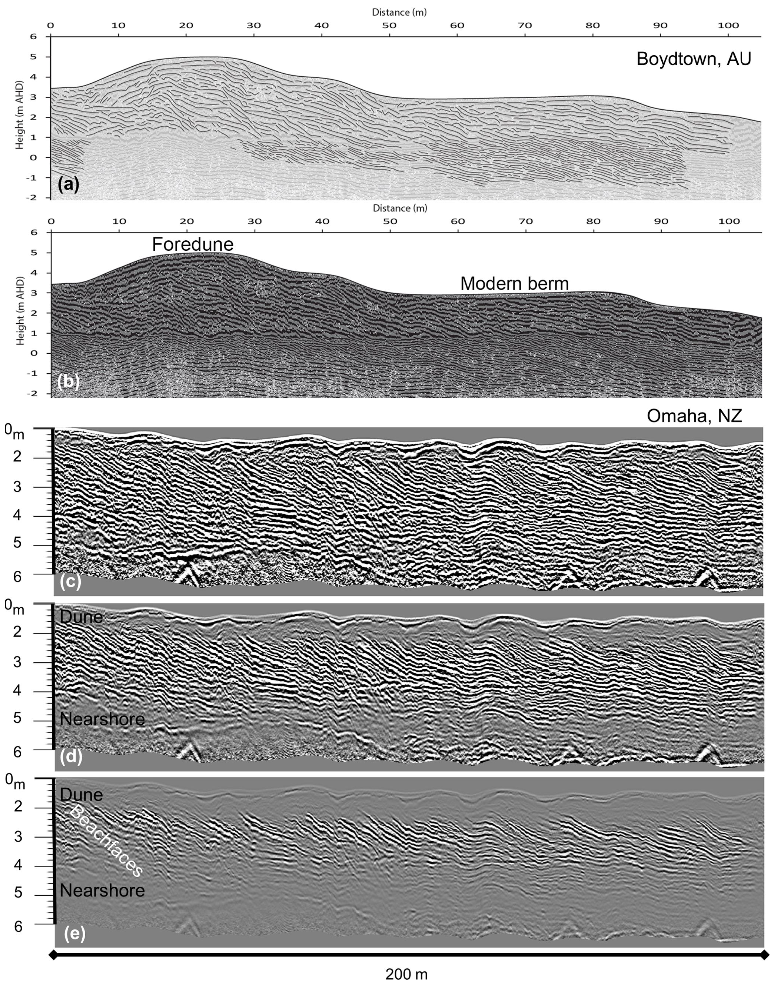
\includegraphics[width=0.9\linewidth]{Figures/0.2GPR/dougherty2019-2.png}
    \caption[Shoreline evolution (2).]{Shoreline evolution (2). \textbf{Keywords: } Prograding, clinoforms, sigmoidal, dipping, tabular, sub-horizontal, concave, downlap, ridge, continuous, semi-continuous, laterally extensive, varied amplitude, truncation, onlap \citep{Dougherty2019}.}
    \label{fig:dougherty2019-2}
\end{figure}

\begin{figure}[h!]
    \centering
    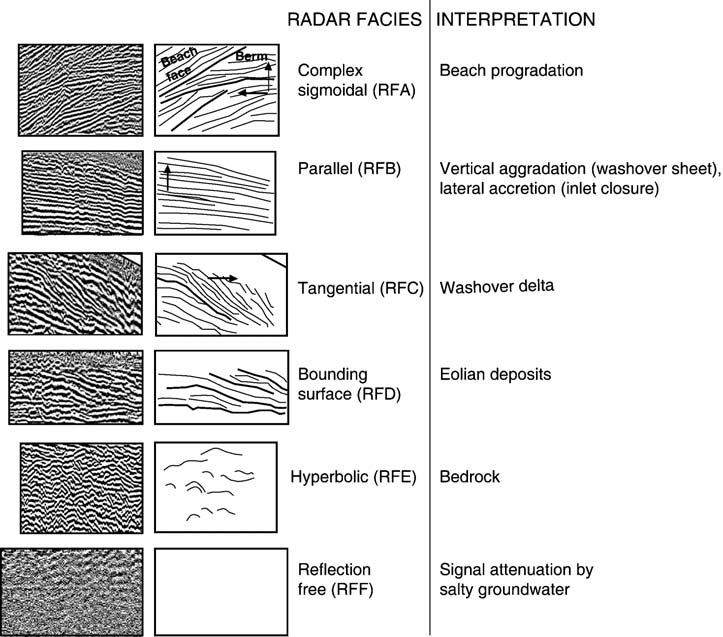
\includegraphics[width=0.9\linewidth]{Figures/0.2GPR/Costas2006_trace_1.png}
    \caption[Transgressive sand barrier (1).]{Transgressive sand barrier (1).\textbf{Keywords: } Sigmoidal, parallel, tangential, bounding surface, hyperbolic, dipping, high attenuation, low reflectivity, high reflectivity \citep{Costas2006}.}
    \label{fig:Costas2006-1}
\end{figure}

\begin{landscape}
\begin{figure}[h!]
    \centering
    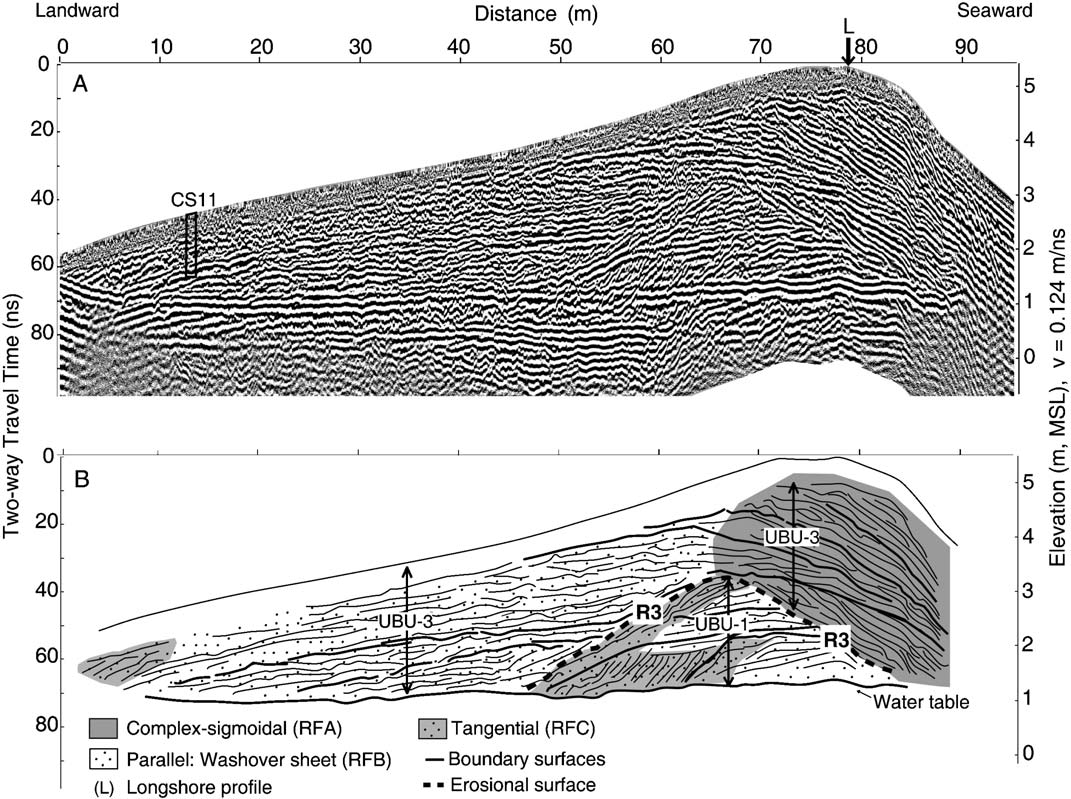
\includegraphics[width=0.8\linewidth]{Figures/0.2GPR/Costas2006_trace_2.png}
    \caption[Transgressive sand barrier (2).]{Transgressive sand barrier (2). \textbf{Keywords: } Parallel, tangential, multidirectional dipping, horizontal, erosion, high reflectivity, low attenuation, bounding surface, sigmoidal, semi-continuous, discontinuous \citep{Costas2006}.}
    \label{fig:Costas2006-2}
\end{figure}
\end{landscape}

\begin{figure}[h!]
    \centering
    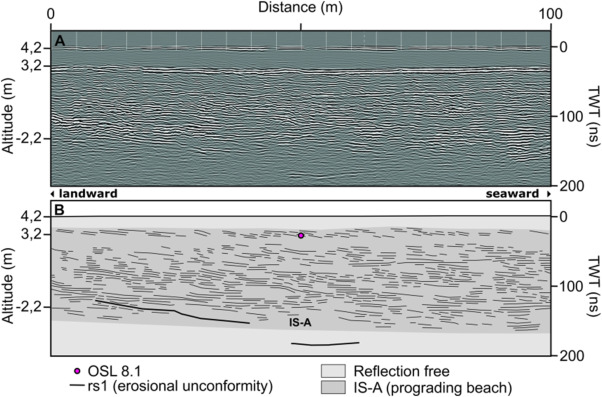
\includegraphics[width=0.8\linewidth]{Figures/0.2GPR/Figueiredo2021-gr4.jpg}
    \caption[Prograding beach ridge.]{Prograding beach ridge. \textbf{Keywords: } Prograding, clinoform, horizontal, dipping, tabular, semi-continuous, high reflectivity, medium reflectivity, high amplitude, moderate amplitude, downlap, onlap \citep{Figueiredo2021}.}
    \label{fig:Figueiredo2021-4}
\end{figure}

\begin{figure}[h!]
    \centering
    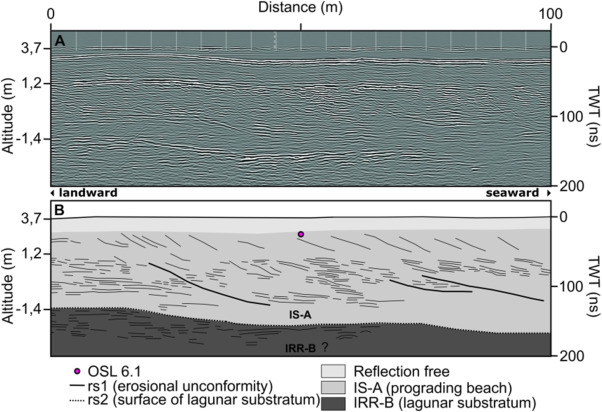
\includegraphics[width=0.8\linewidth]{Figures/0.2GPR/Figueiredo2021-gr5.jpg}
    \caption[Prograding beach ridge.]{Prograding beach ridge. \textbf{Keywords: } Sigmoidal, convex, continuous, medium reflectivity, high reflectivity, low amplitude, truncation, prograding, dipping \citep{Figueiredo2021}.}
    \label{fig:Figueiredo2021-5}
\end{figure}

\begin{landscape}
\begin{figure}[h!]
    \centering
    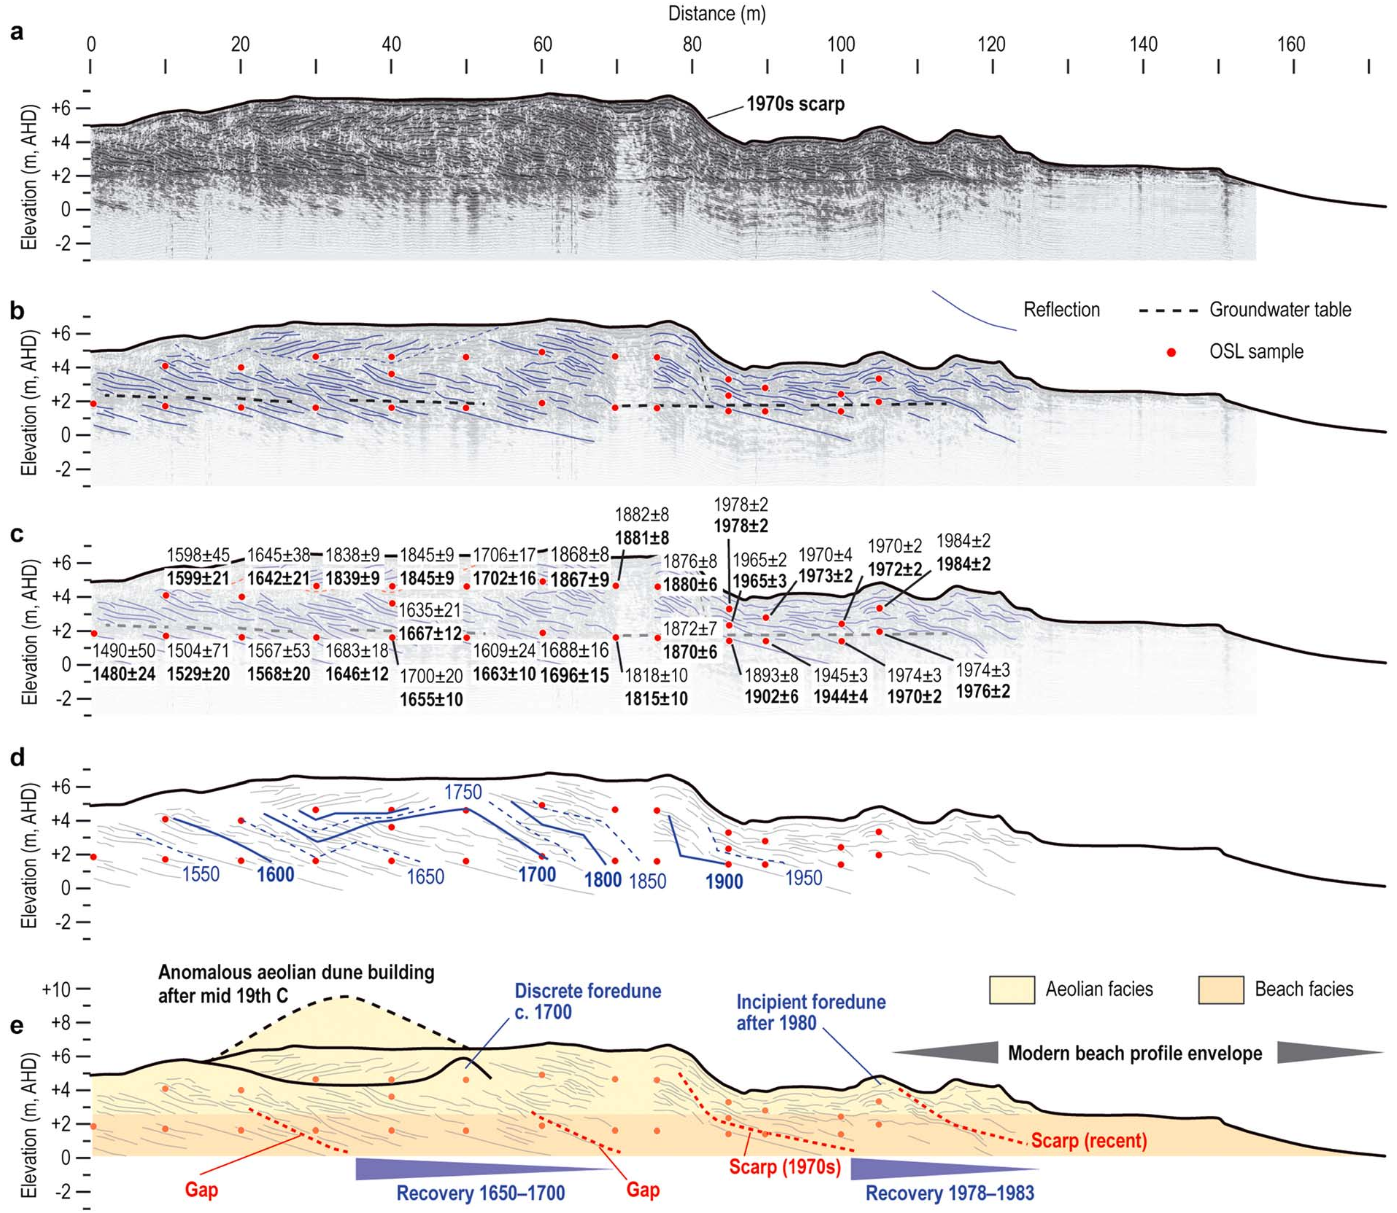
\includegraphics[width=0.75\linewidth]{Figures/0.2GPR/Tamura_2019_BR_Coast_er_1.png}
    \caption[Beach ridges and coastal erosion.]{Beach ridges and coastal erosion. \textbf{Keywords: } Dipping, continuous, semi-continuous, moderate amplitude, varied reflectivity, downlap, progradation, truncation, onlap, erosion \citep{Tamura2019}.}
    \label{fig:Tamura2019-1}
\end{figure}
\end{landscape}

\begin{landscape}
\begin{figure}[h!]
    \centering
    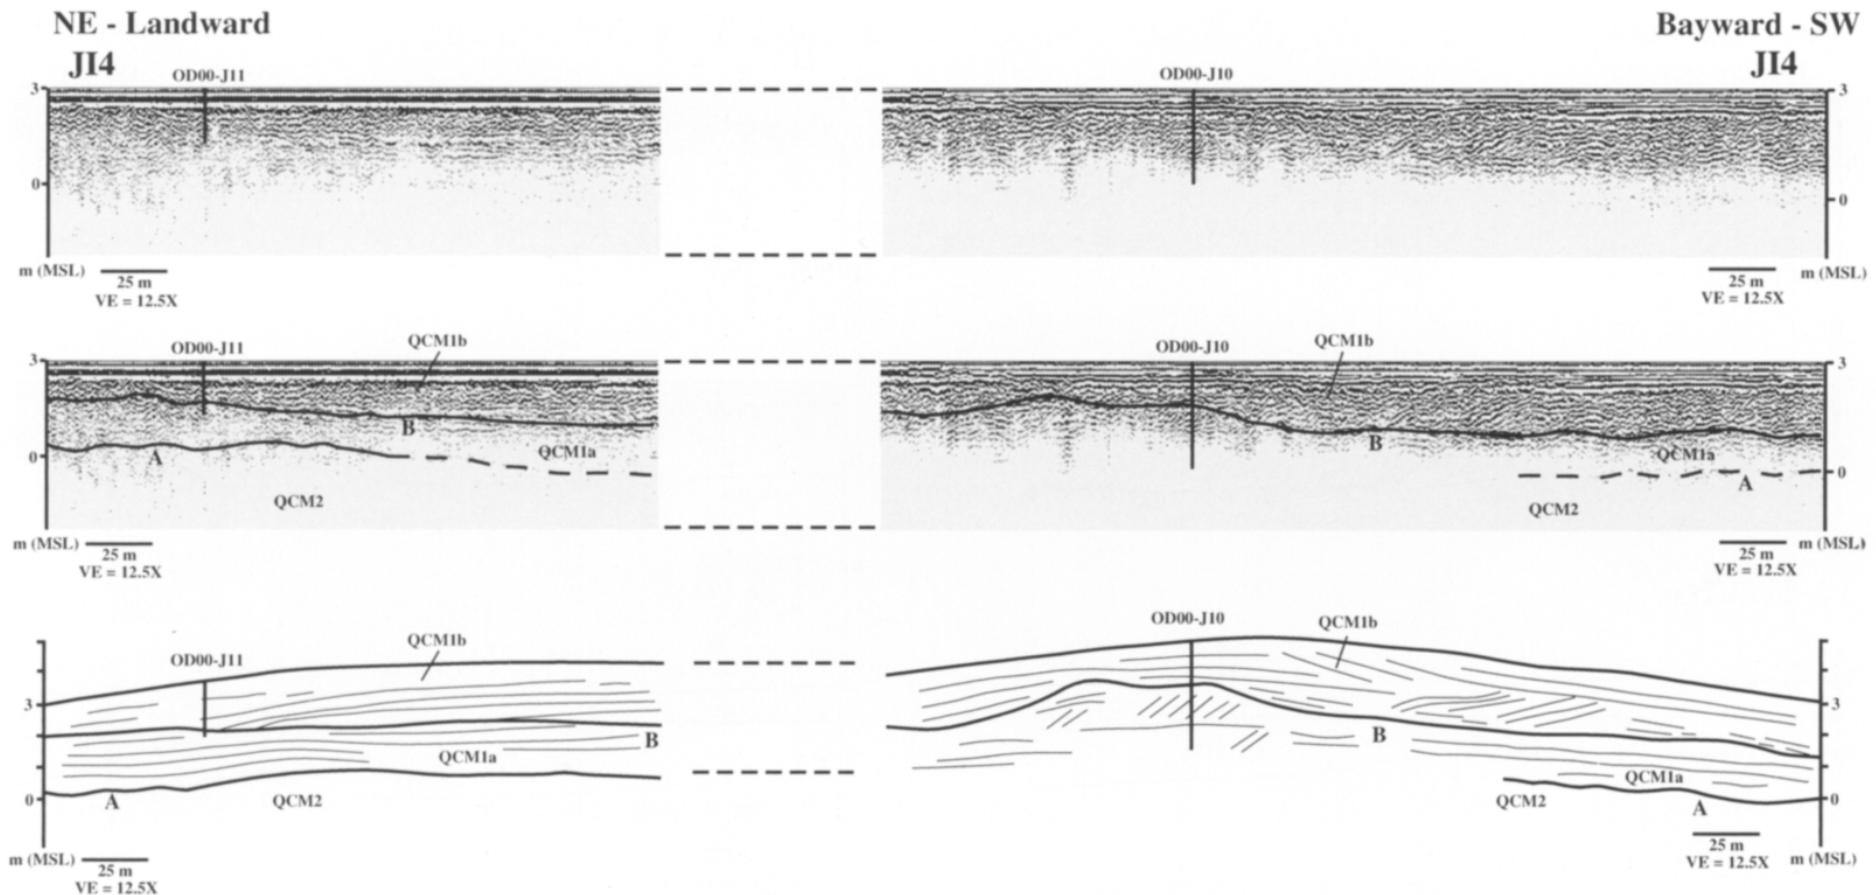
\includegraphics[width=0.9\linewidth]{Figures/0.2GPR/neal2003_1.png}
    \caption[Coarse-clastic beach-ridge deposits (1).]{Coarse-clastic beach-ridge deposits (1). \textbf{Keywords: } Dipping, tabular, semi-continuous, high amplitude, medium amplitude, truncation, downlap, prograding, onlap \citep{Neal2003}.}
    \label{fig:Neal2003-1}
\end{figure}
\end{landscape}

\begin{landscape}
  \begin{figure}[h!]
    \centering
    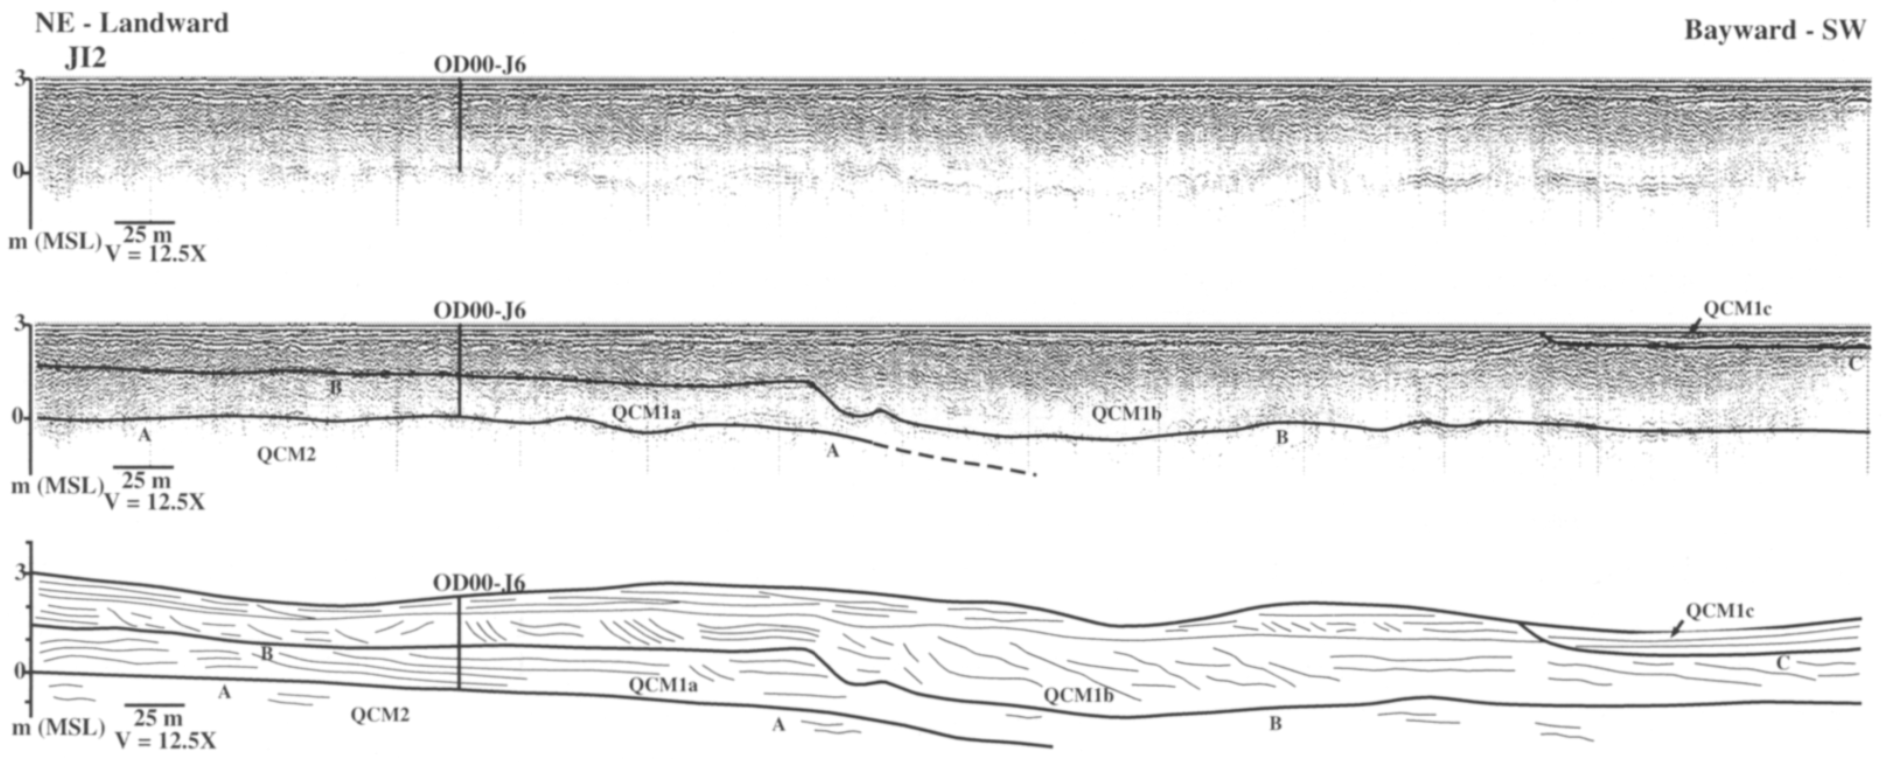
\includegraphics[width=0.9\linewidth]{Figures/0.2GPR/neal2003_2.png}
    \caption[Coarse-clastic beach-ridge deposits (2).]{Coarse-clastic beach-ridge deposits (2).\textbf{Keywords: } Sub-horizontal, lenticular, dipping, discontinuous, continuous, low amplitude, low reflectivity, high amplitude, erosion, bounding \citep{Neal2003}.}
    \label{fig:Neal2003-2}
\end{figure}  
\end{landscape}

\begin{figure}[h!]
    \centering
    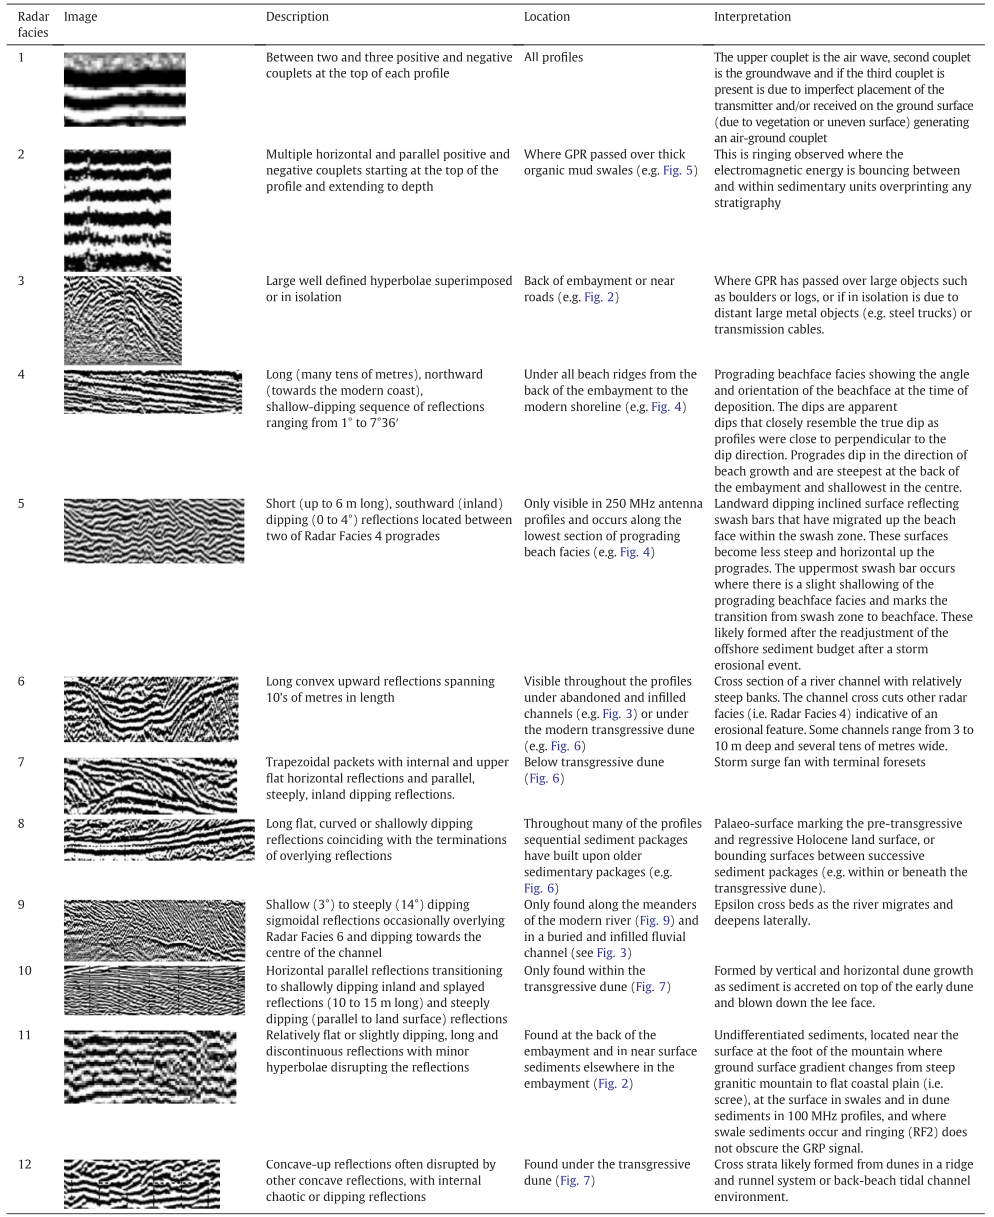
\includegraphics[width=0.9\linewidth]{Figures/0.2GPR/Gourmanis2020_coastal.png}
    \caption[Holocene evolution of coastal embayment.]{Holocene evolution of coastal embayment. \textbf{Keywords: } Horizontal, parallel, hyperbola, dipping, prograding, convex, horizontal, curved, sigmoidal, discontinuous, chaotic, semi-continuous, high reflectivity, low reflectivity \citep{Guramanis2020}.}
    \label{fig:Gourmanis2020-1}
\end{figure}

\begin{figure}[h!]
    \centering
    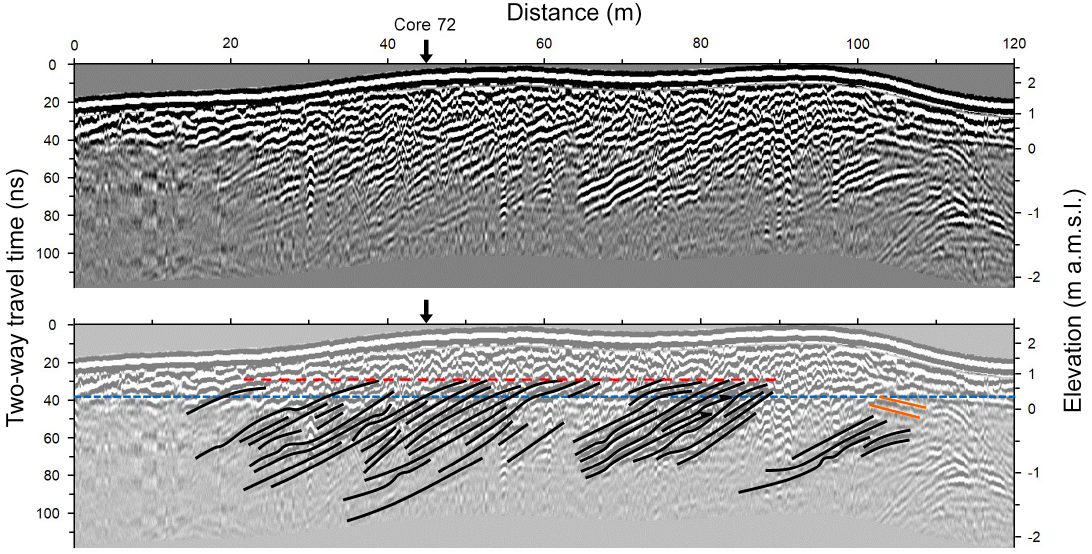
\includegraphics[width=0.9\linewidth]{Figures/0.2GPR/Nooren_2017_beach.png}
    \caption[Beach ridge plain.]{Beach ridge plain. \textbf{Keywords: } Dipping, parallel, erosion, semi-continuous, discontinuous, chaotic, high reflectivity, low reflectivity \citep{Nooren2017}.}
    \label{fig:Nooren2017-1}
\end{figure}

\begin{figure}[h!]
    \centering
    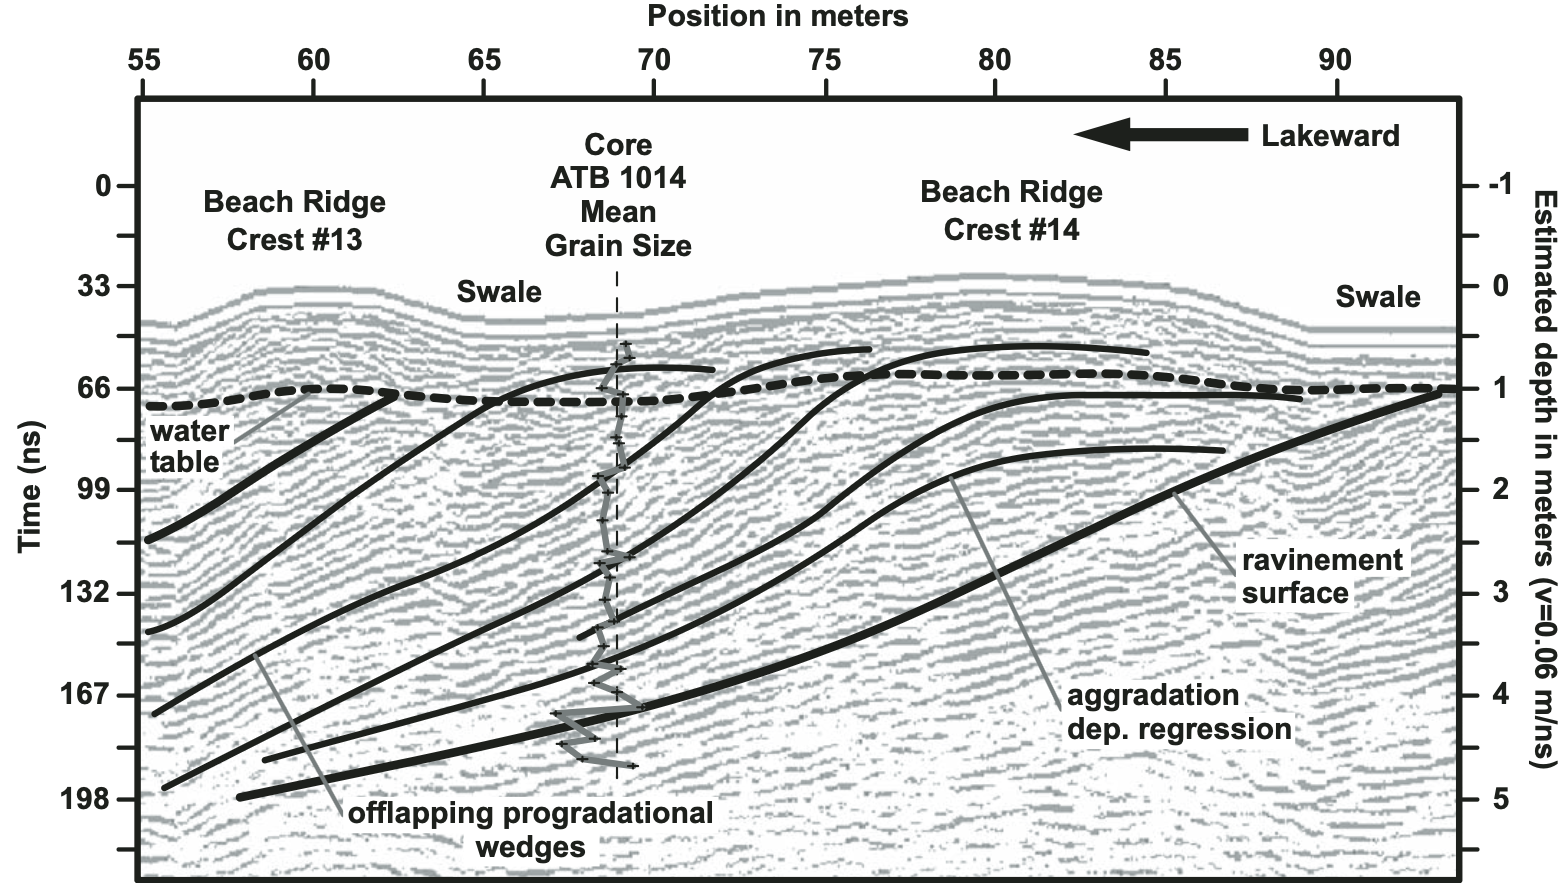
\includegraphics[width=0.9\linewidth]{Figures/0.2GPR/Johnston2007-2.png}
    \caption[Beach ridge development.]{Beach ridge development. \textbf{Keywords: } Dipping, continuous, discontinuous, parallel, hummocky, erosion, high reflectivity, low reflectivity \citep{Johnston2007}.}
\end{figure} 


\begin{figure}[h!]
    \centering
    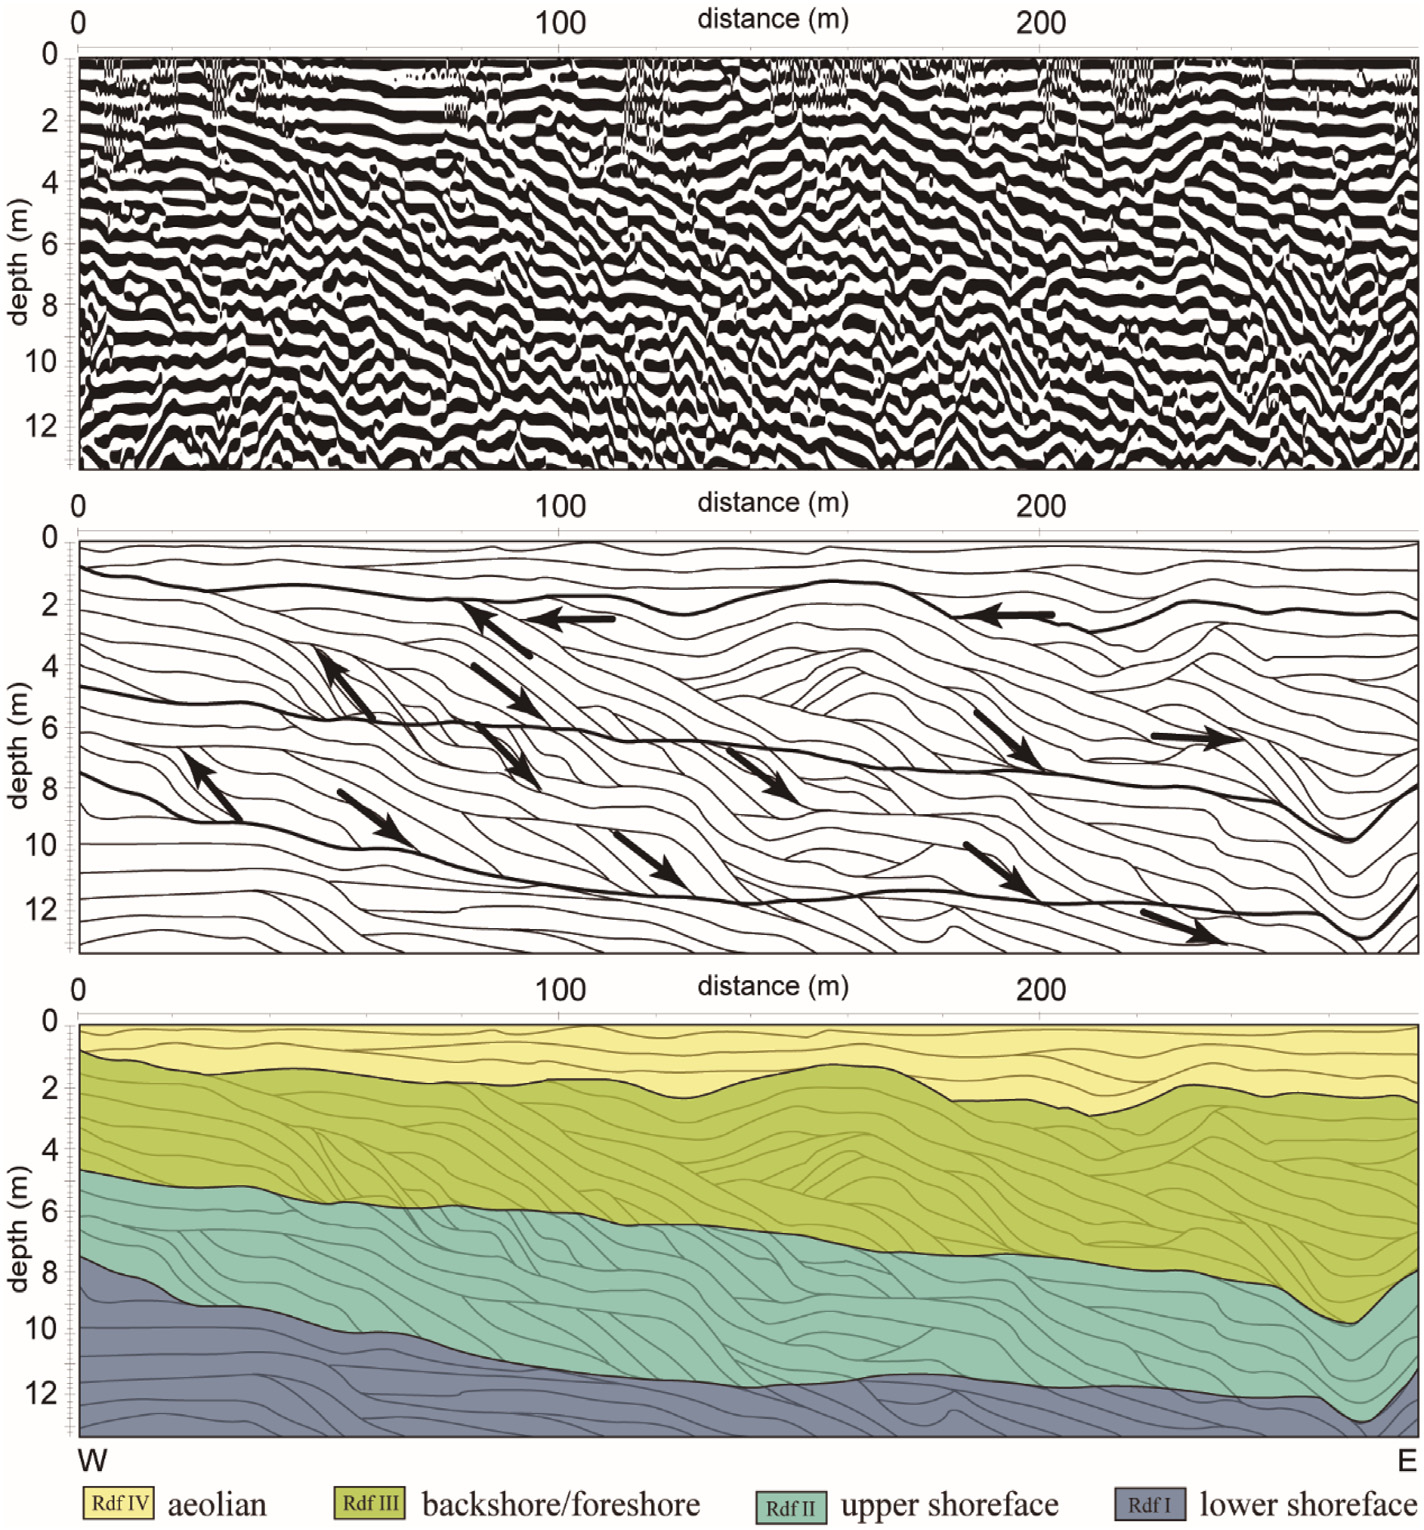
\includegraphics[width=0.9\linewidth]{Figures/0.2GPR/Leandro2018_coastal_2.png}
    \caption[Coastal depositional environments.]{Coastal depositional environments. \textbf{Keywords: } Erosional, dipping, chaotic, hummocky, onlap, downlap, truncation, high reflectivity, semi-horizontal, semi-parallel \citep{Leandro2019}.}
    \label{fig:Leandro2019-2}
\end{figure}

\begin{landscape}
    \begin{figure}[h!]
    \centering
    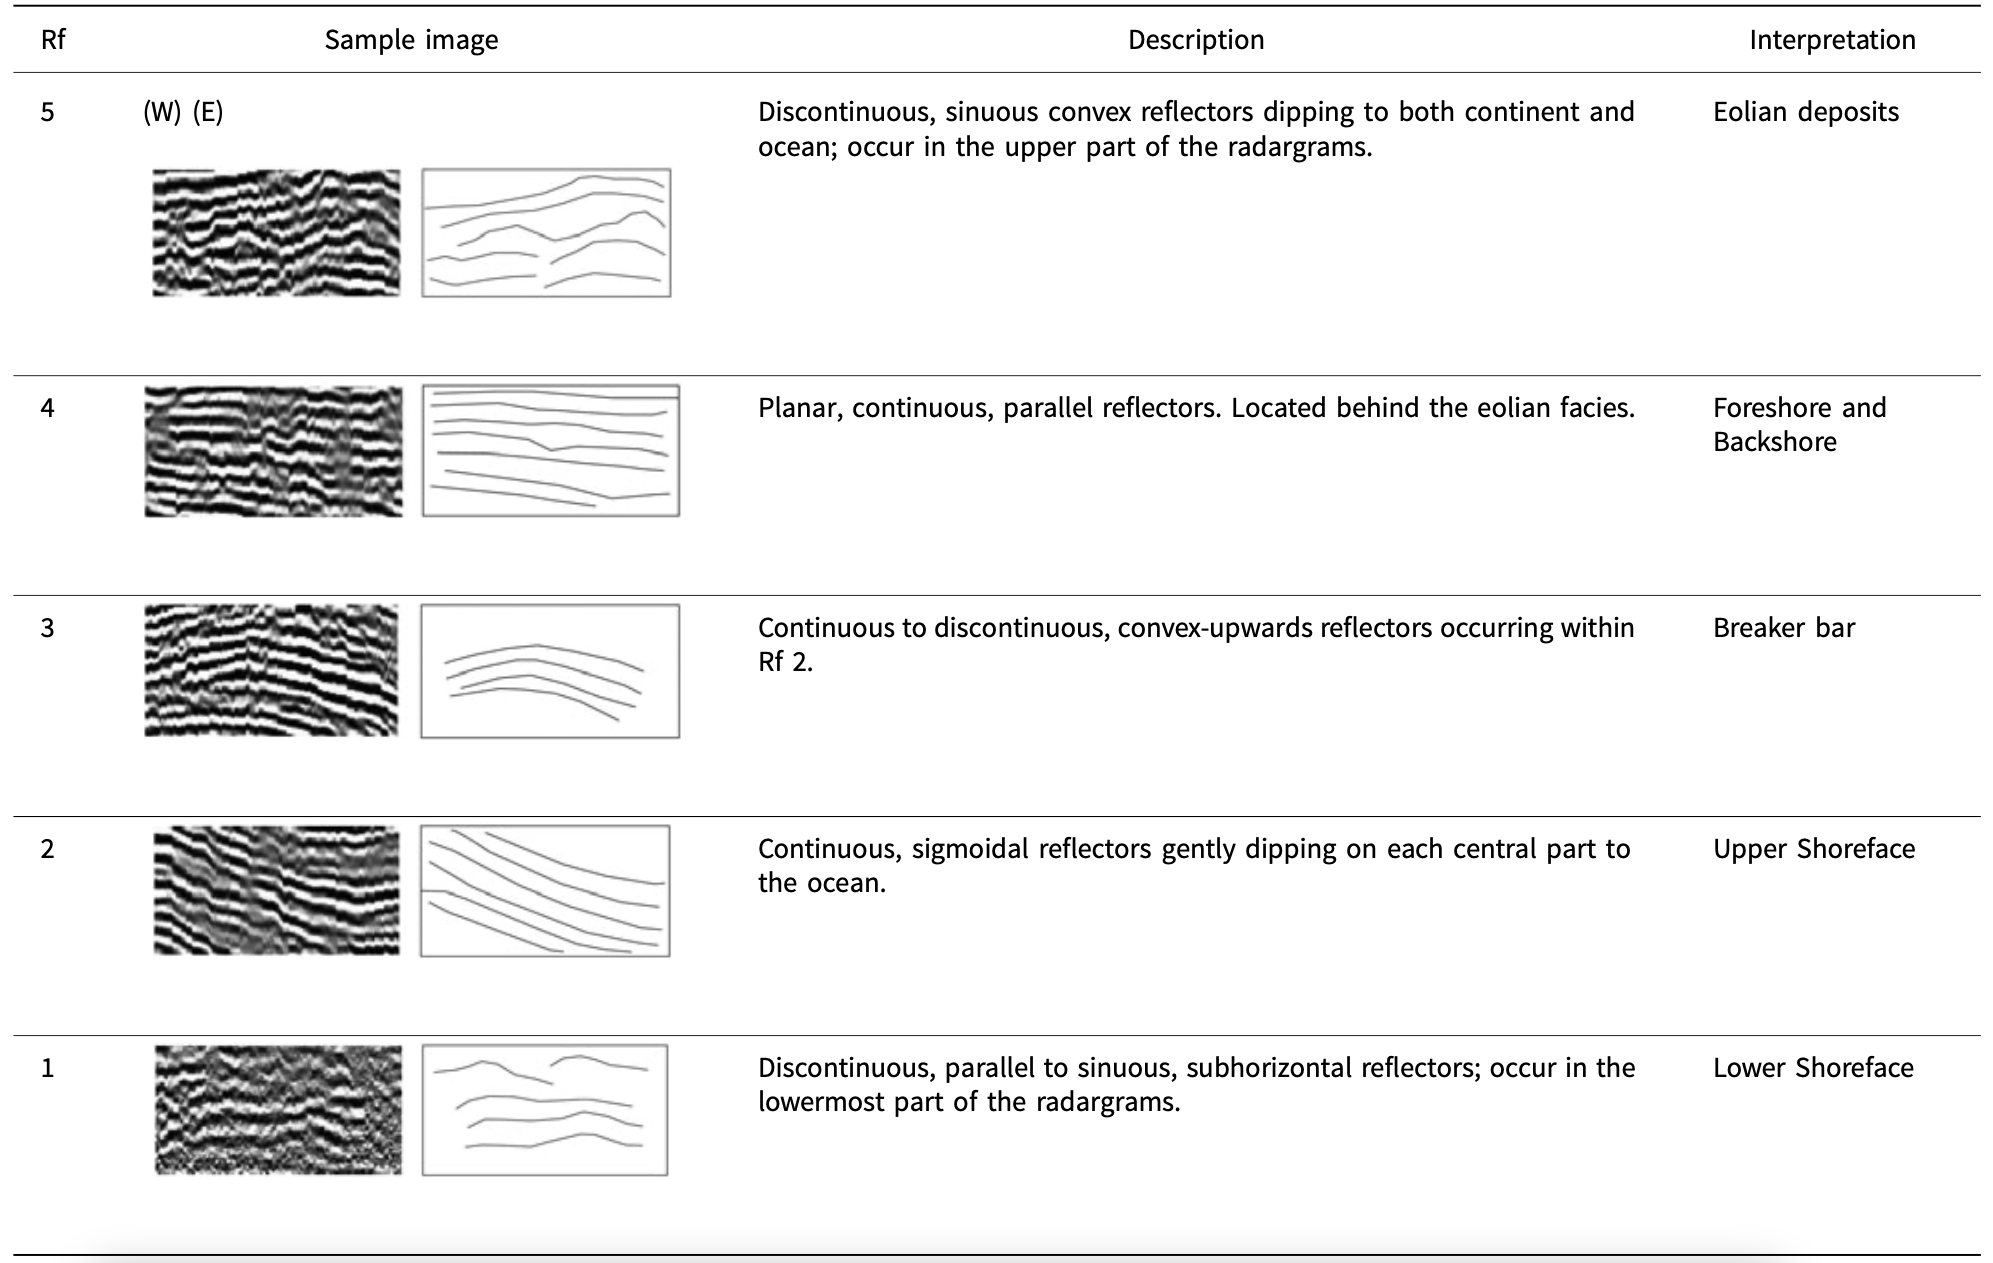
\includegraphics[width=0.9\linewidth]{Figures/0.2GPR/Santos2022_2.png}
    \caption[Micro-tidal barrier.]{Micro-tidal barrier. \textbf{Keywords: } Discontinuous, sinuous, convex, dipping, planar, continuous, sigmoidal, parallel, subhorizontal \citep{Santos2022}.}
    \label{fig:Santos2022-2}
\end{figure}
\end{landscape}

\begin{figure}[h!]
    \centering
    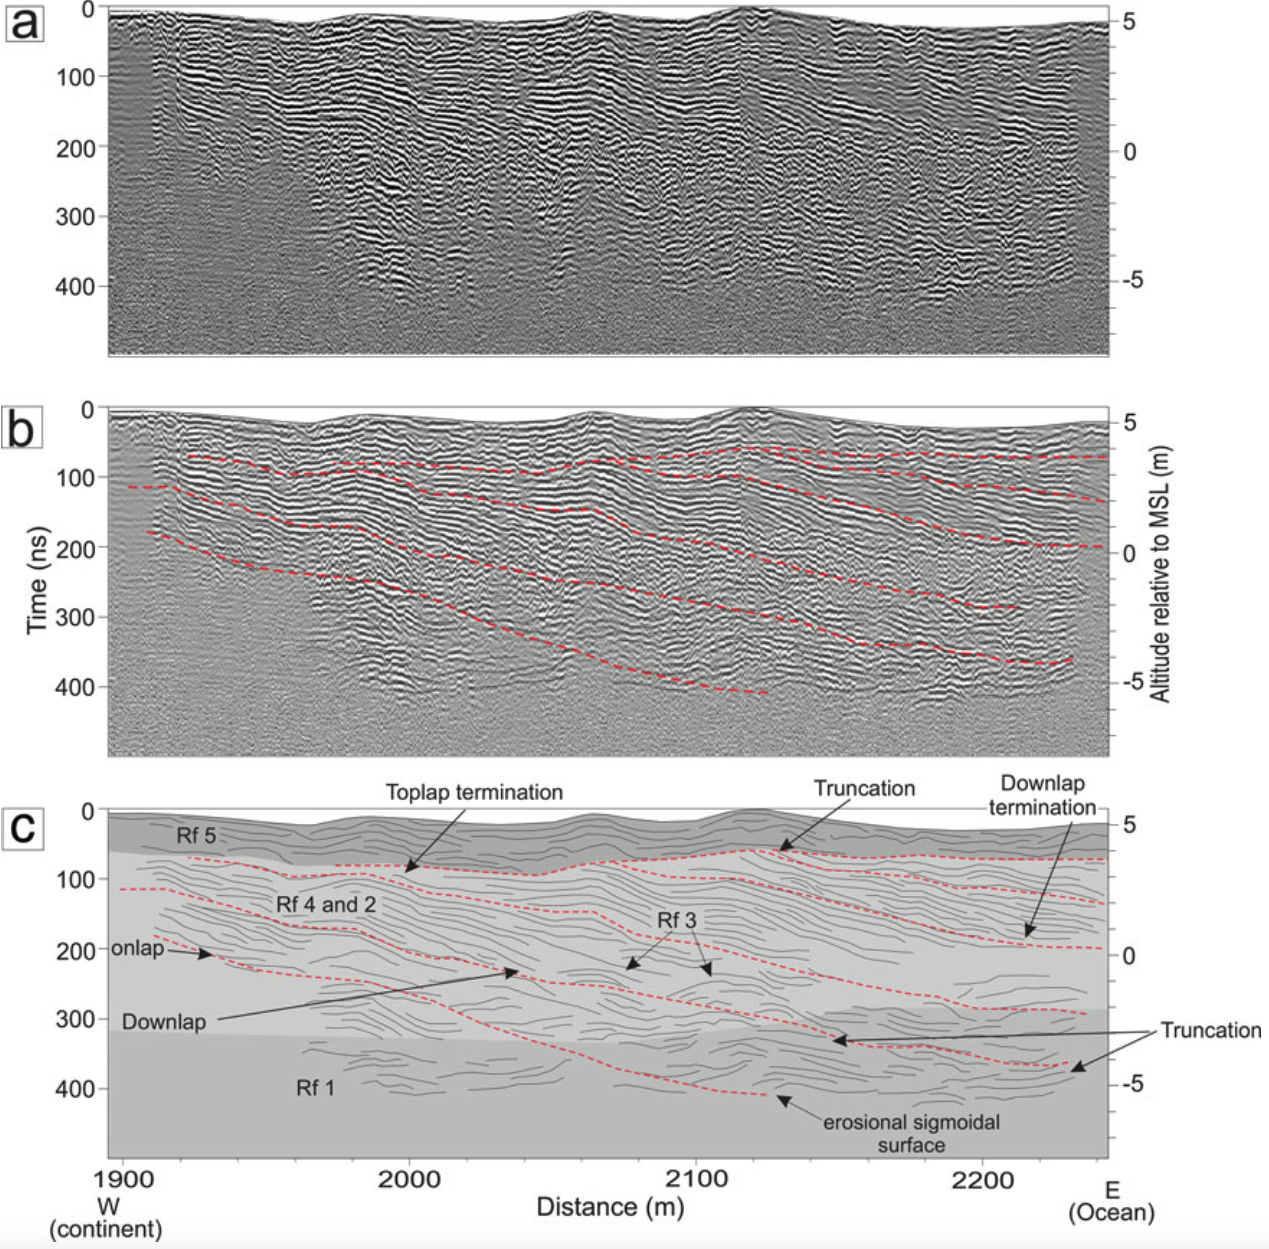
\includegraphics[width=0.9\linewidth]{Figures/0.2GPR/Santos2022_3.png}
    \caption[Micro-tidal barrier.]{Micro-tidal barrier. \textbf{Keywords: } Sigmoidal, truncation, downlap, toplap, and onlap \citep{Santos2022}.}
    \label{fig:Santos2022-3}
\end{figure}

\begin{landscape}
\begin{figure}[h!]
    \centering
    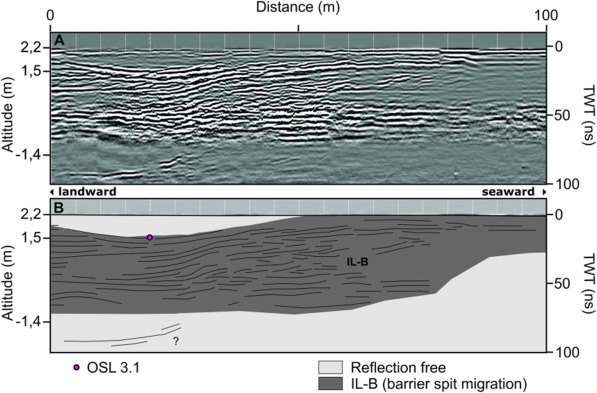
\includegraphics[width=0.9\linewidth]{Figures/0.2GPR/Figueiredo2021-gr8.jpg}
    \caption[Late Holocene evolution of sedimentary cape.]{Late Holocene evolution of sedimentary cape. \textbf{Keywords: } Discontinuous, varied reflectivity, semi-horizontal, chaotic, semi-parallel, slight dipping \citep{Figueiredo2021}.}
    \label{fig:Figueiredo2021-8}
\end{figure}
\end{landscape}
\clearpage

\begin{figure}[h!]
    \centering
    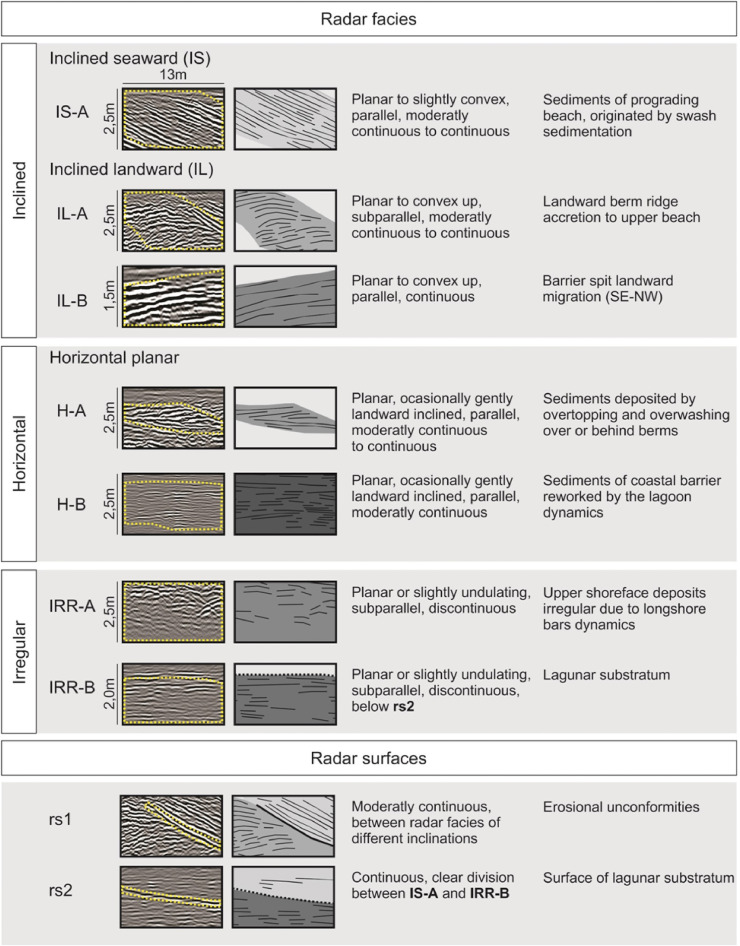
\includegraphics[width=0.9\linewidth]{Figures/0.2GPR/Figueiredo2021-fx1.jpg}
    \caption[Late Holocene evolution of sedimentary cape.]{Late Holocene evolution of sedimentary cape. \textbf{Keywords: } Inclined, horizontal, irregular, planar, convex, parallel, continuous, subparallel, undulating, discontinuous, unconformity, dipping \citep{Figueiredo2021}.}
    \label{fig:Figueiredo2021-1}
\end{figure}
\clearpage

\clearpage
\subsubsection{Eolian}
\begin{table}[h!]
\centering
\caption{Categorised GPR profile keywords for eolian environments. Geometry, reflectivity and continuity are shown in separate columns.}
\begin{tabular}{|p{5cm}|p{5cm}|p{5cm}|}
\hline
\textbf{Geometry / Structure} & \textbf{Continuity} & \textbf{Amplitude / Reflectivity} \\
\hline
Truncation & Semi-continuous & High reflectivity \\
Downlap & Discontinuous & Medium reflectivity \\
Oblique & Moderately continuous & Low reflectivity \\
Subparallel & Medium continuous & High amplitude \\
Horizontal subparallel & Continuous & Medium amplitude \\
Convex & &  \\
Concave & & High attenuation \\
Dipping & & \\
Multidirectional dipping & & \\
Horizontal & & \\
Sub-horizontal & & \\
Parallel & & \\
Tabular & & \\
Hummocky & & \\
Chaotic & & \\
Divergent & & \\
Diffraction hyperbolas & & \\
Tangential & & \\
Sigmoidal & & \\
Bounding surface & & \\
\hline
\end{tabular}
\label{tab:dune-coastal-keywords}
\end{table}

\begin{figure}[h!]
    \centering
    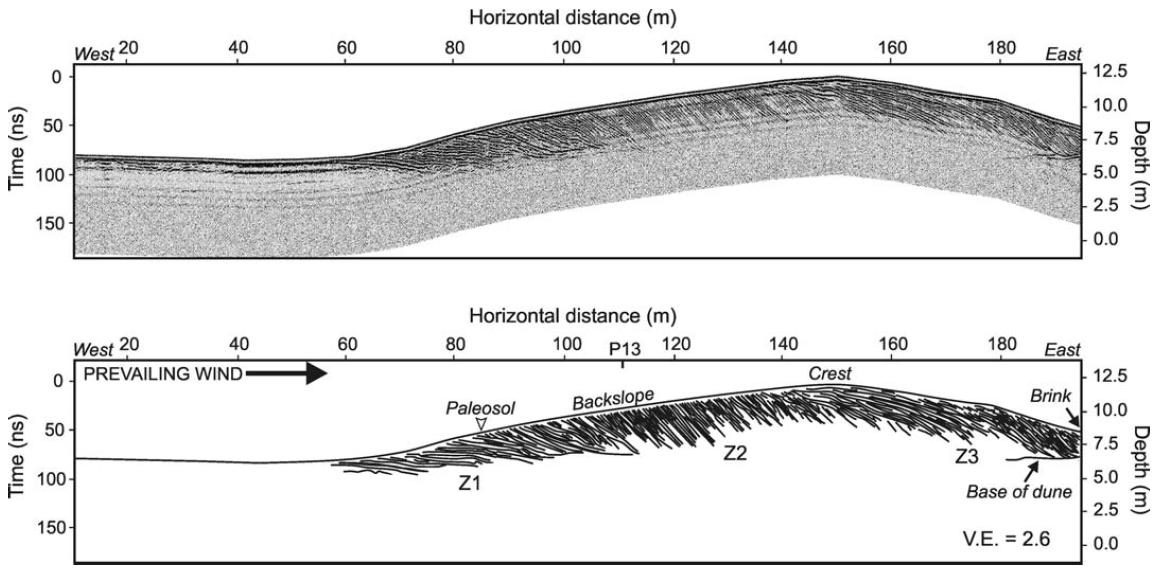
\includegraphics[width=0.9\linewidth]{Figures/0.2GPR/Hugenholtz_2007_1.png}
    \caption[Parabolic sand dune (2)]{Parabolic sand dune (2). \textbf{Keywords: } Truncation, downlap, oblique, subparallel, concave, dipping \citep{Hugenholtz2007}.}
    \label{fig:Hugenholtz2007-1}
\end{figure}

\begin{figure}[h!]
    \centering
    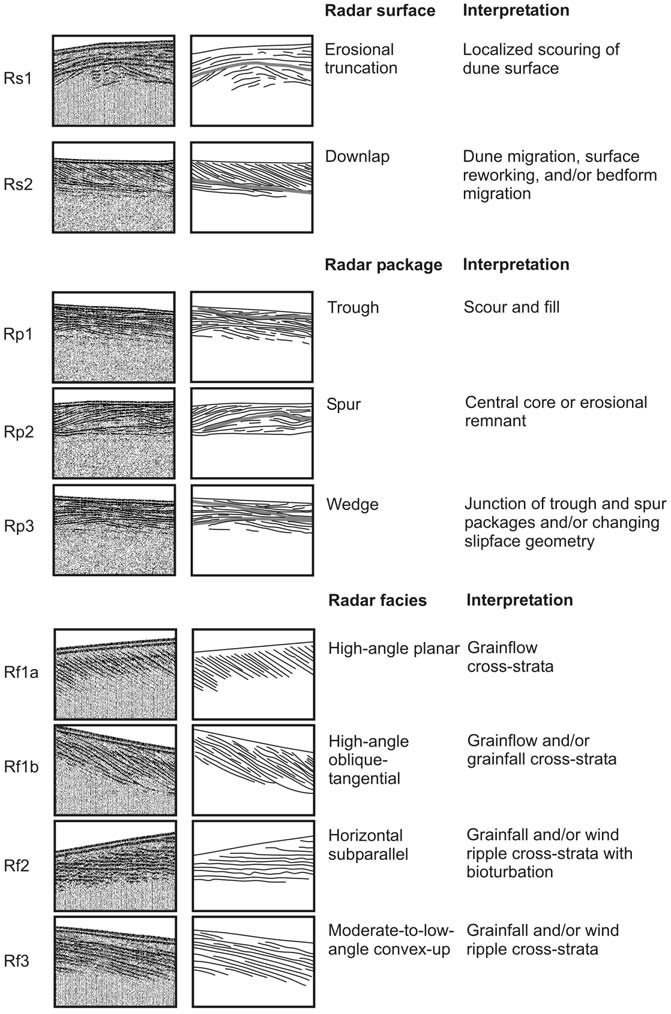
\includegraphics[width=0.9\linewidth]{Figures/0.2GPR/Hugenholtz2007_parabolicdunes.png}
    \caption[Parabolic sand dune (1).]{Parabolic sand dune (1). \textbf{Keywords: } Truncation, downlap, oblique, horizontal subparallel, convex, dipping \citep{Hugenholtz2007}.}
    \label{fig:Hugenholtz2007-4}
\end{figure}
\clearpage

\begin{figure}[h!]
    \centering
    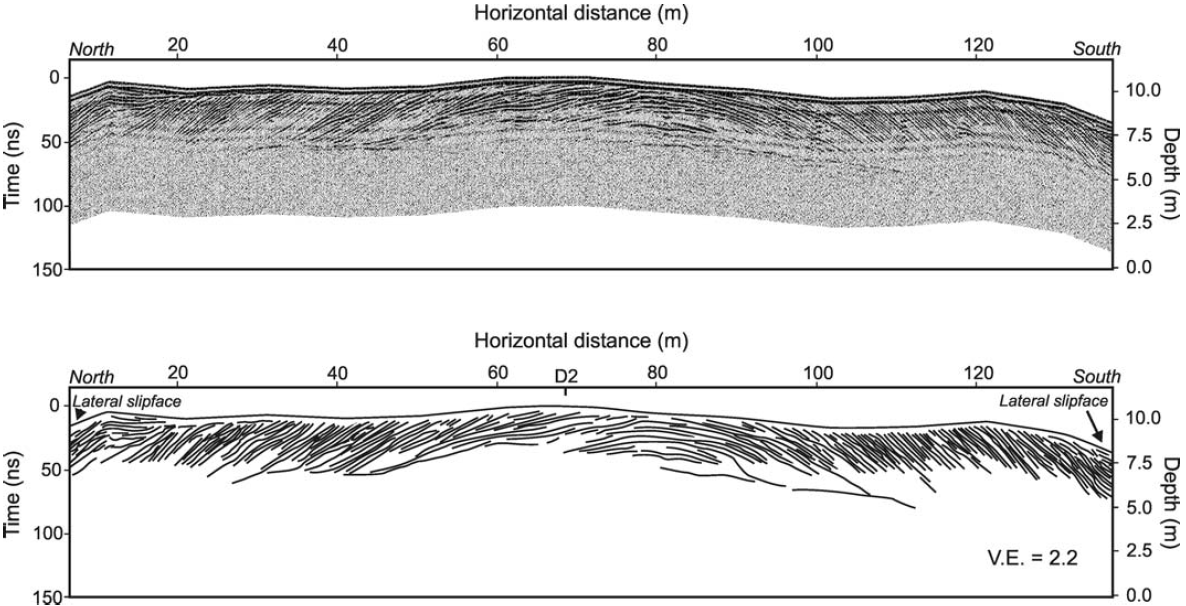
\includegraphics[width=0.9\linewidth]{Figures/0.2GPR/Hugenholtz_2007_3.png}
    \caption[Parabolic sand dune (3).]{Parabolic sand dune (3). \textbf{Keywords: } Truncation, downlap, oblique, subparallel, concave, multidirectional dipping \citep{Hugenholtz2007}.}
    \label{fig:Hugenholtz2007-3}
\end{figure}

\begin{figure}[h!]
    \centering
    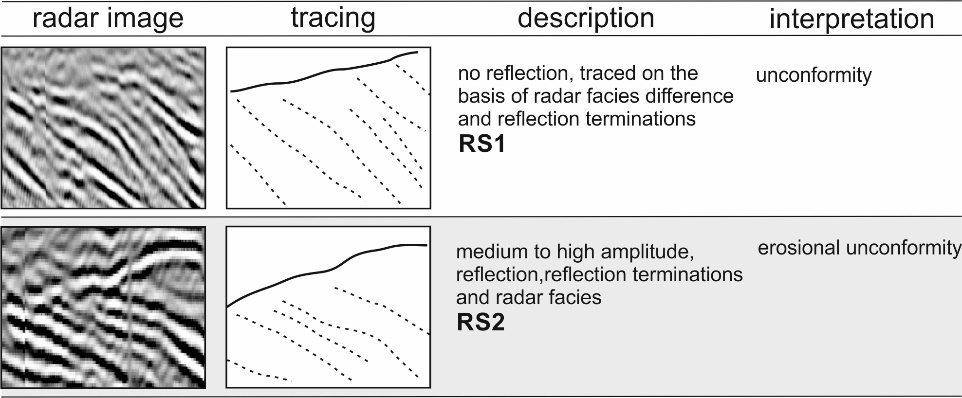
\includegraphics[width=0.9\linewidth]{Figures/0.2GPR/Ribolini2021_dunes_1.png}
    \caption[Coastal dunes (1).]{Coastal dunes (1). \textbf{Keywords: } Dipping, horizontal, convex, concave, chaotic, high attenuation, medium amplitude, high amplitude, moderately continuous, continuous, divergent, low amplitude, sub-horizontal, discontinuous, diffraction hyperbolas. \citep{Ribolini2021}.}
    \label{fig:Ribolini2021-1}
\end{figure}


\begin{figure}[h!]
    \centering
    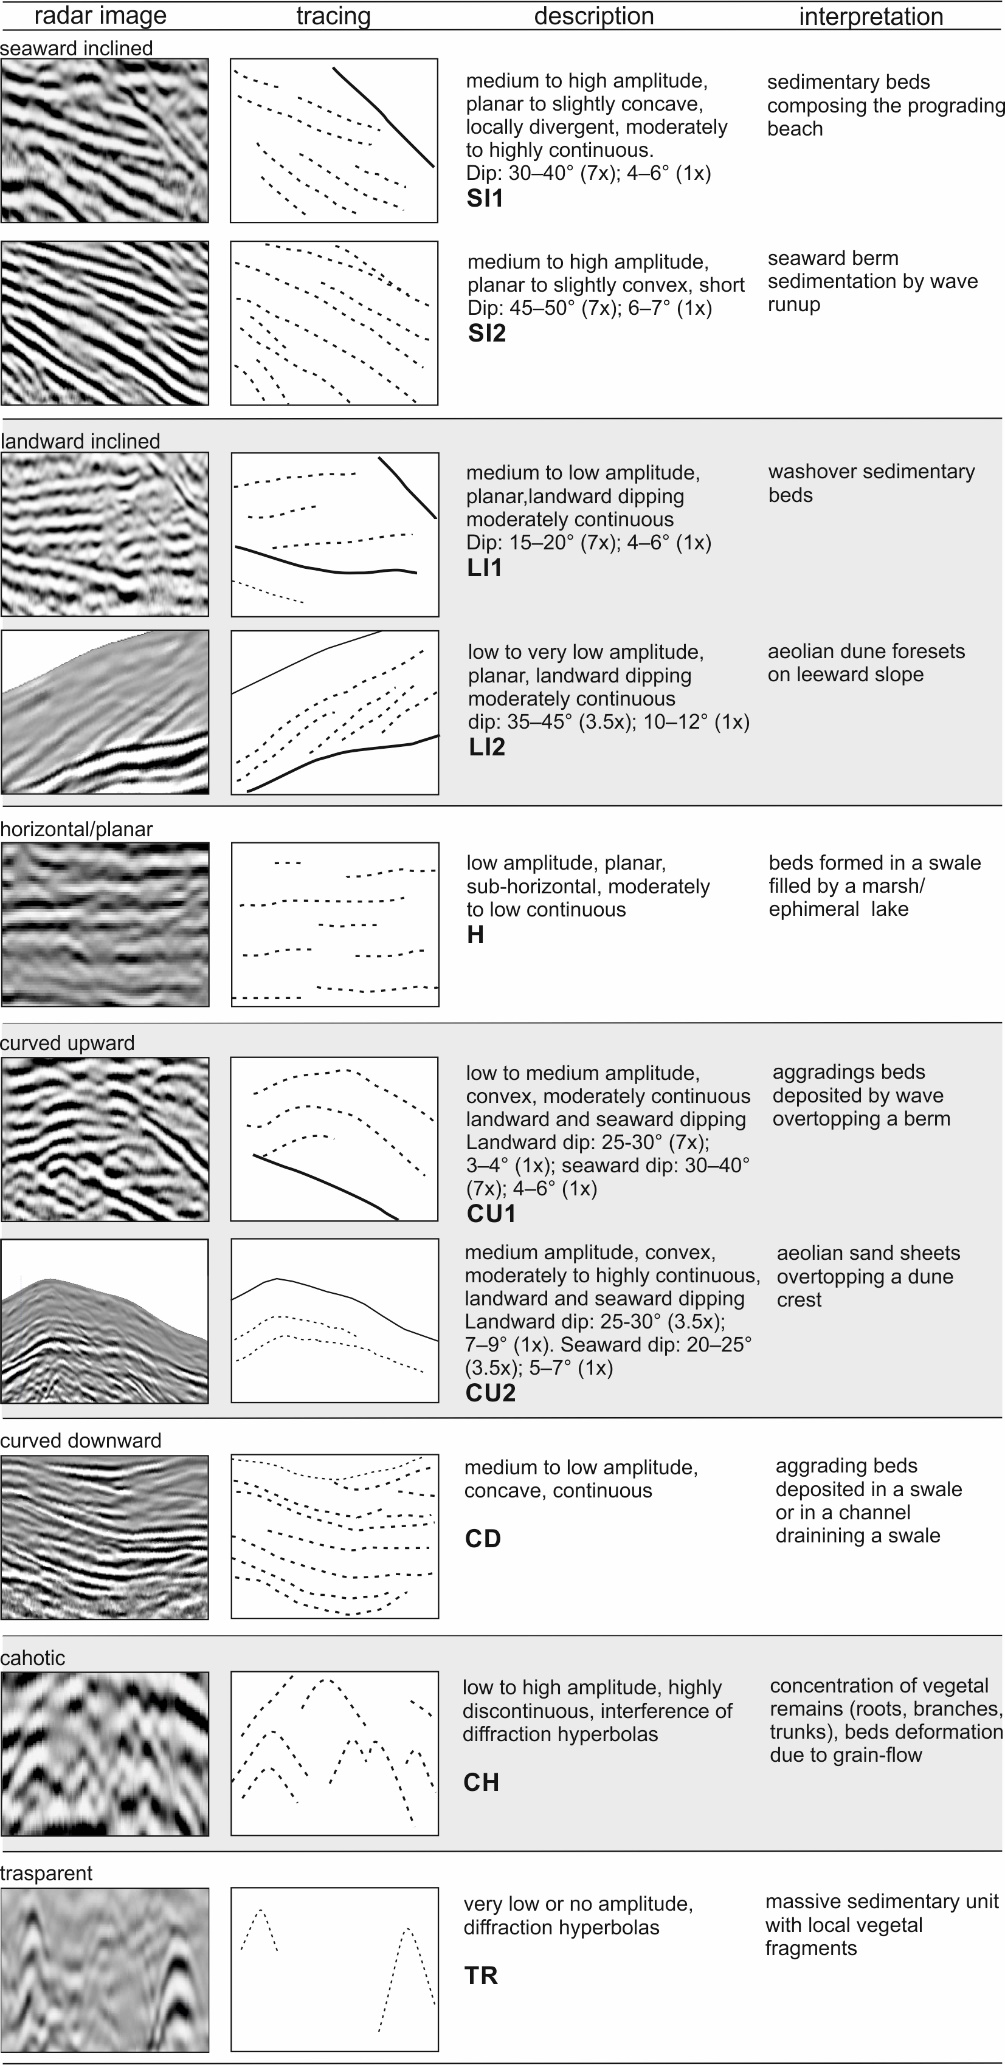
\includegraphics[width=0.75\linewidth]{Figures/0.2GPR/Ribolini2021_dunes_2.png}
    \caption[Coastal dunes (2).]{Coastal dunes (2).\textbf{Keywords: } Medium amplitude, high amplitude, concave, medium continuous, low amplitude, sub-horizontal, discontinuous, diffraction hyperbolas, high attenuation \citep{Ribolini2021}.}
    \label{fig:Ribolini2021-2}
\end{figure}


\clearpage
\begin{landscape}
    \begin{figure}[h!]
    \centering
    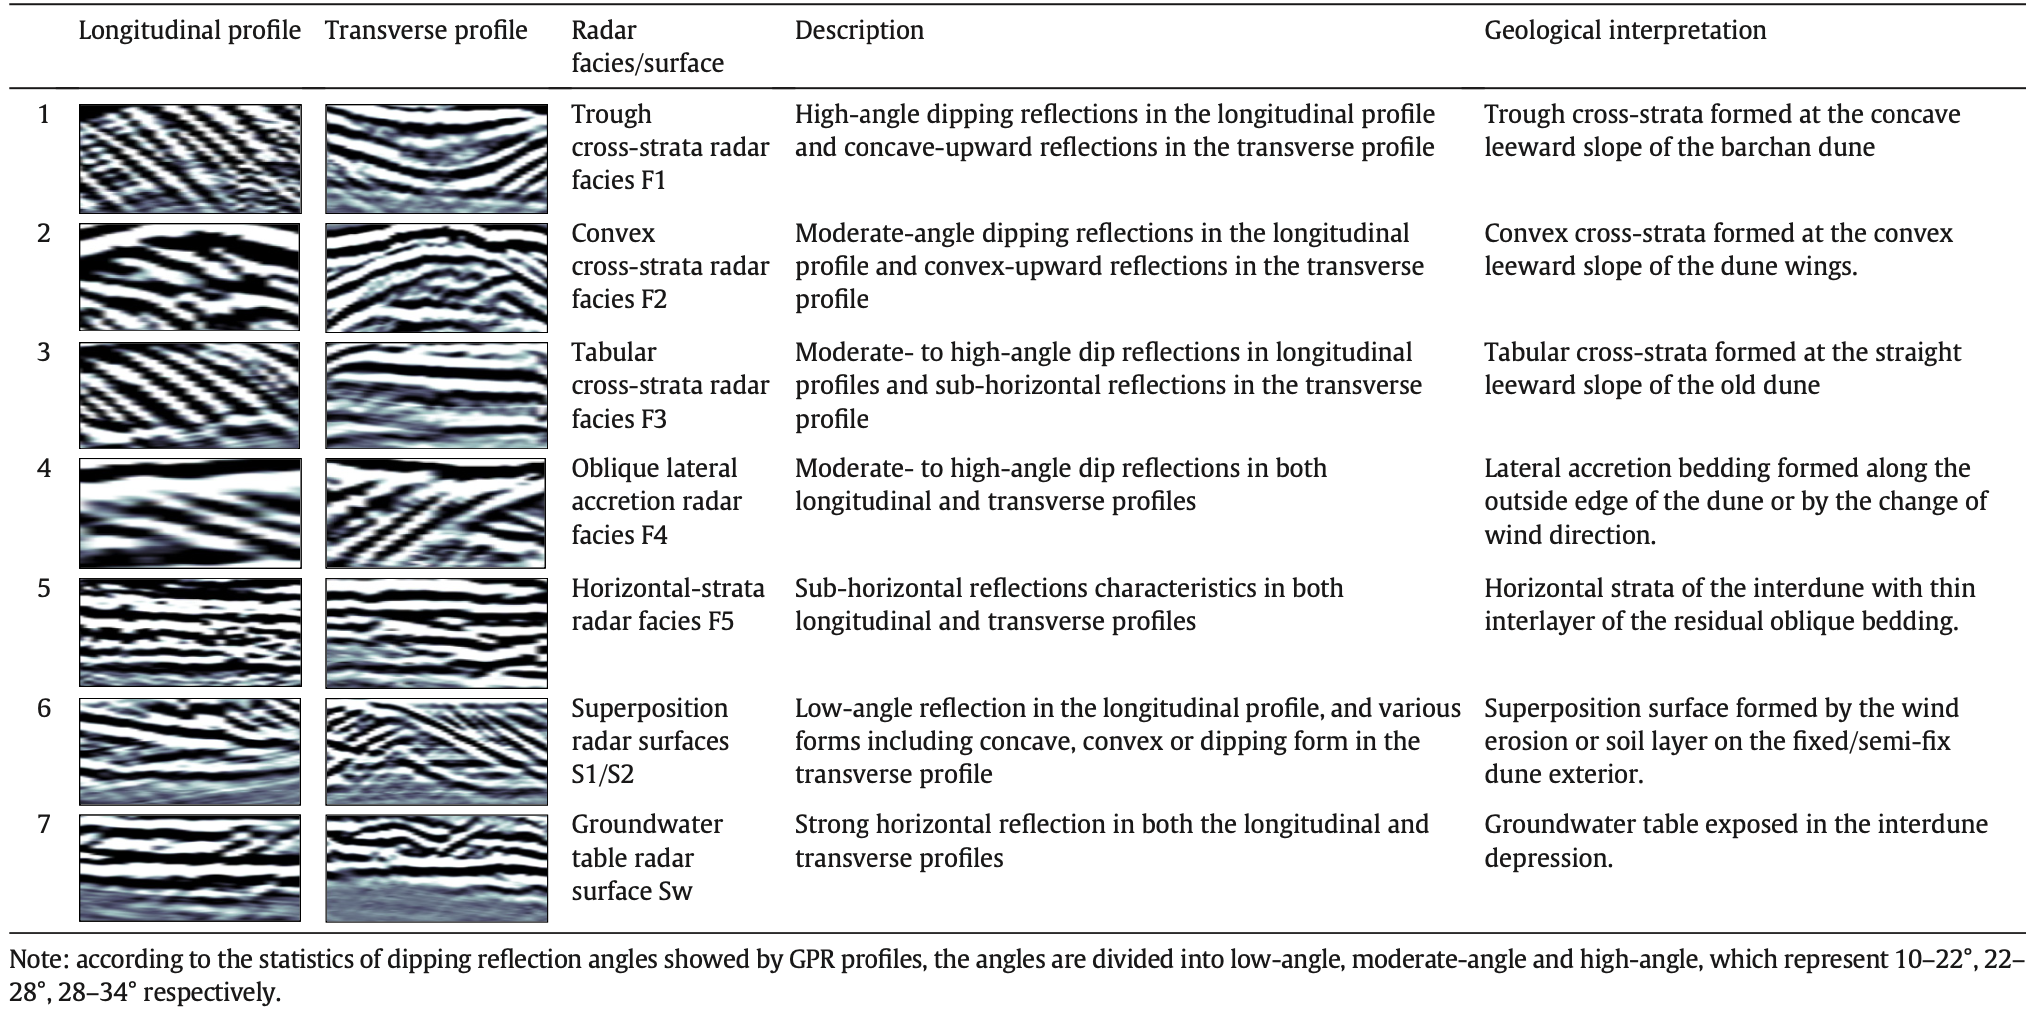
\includegraphics[width=0.8\linewidth]{Figures/0.2GPR/Fu_2019_dunes_1.png}
    \caption[Barchan dune (1).]{Barchan dune (1). \textbf{Keywords: } Dipping, concave, convex, sub-horizontal, tabular, horizontal, high reflectivity, medium reflectivity, semi-continuous, discontinuous \citep{Fu2024}.}
    \label{fig:Fu2019-1}
\end{figure}
\end{landscape}

\begin{figure}[h!]
    \centering
    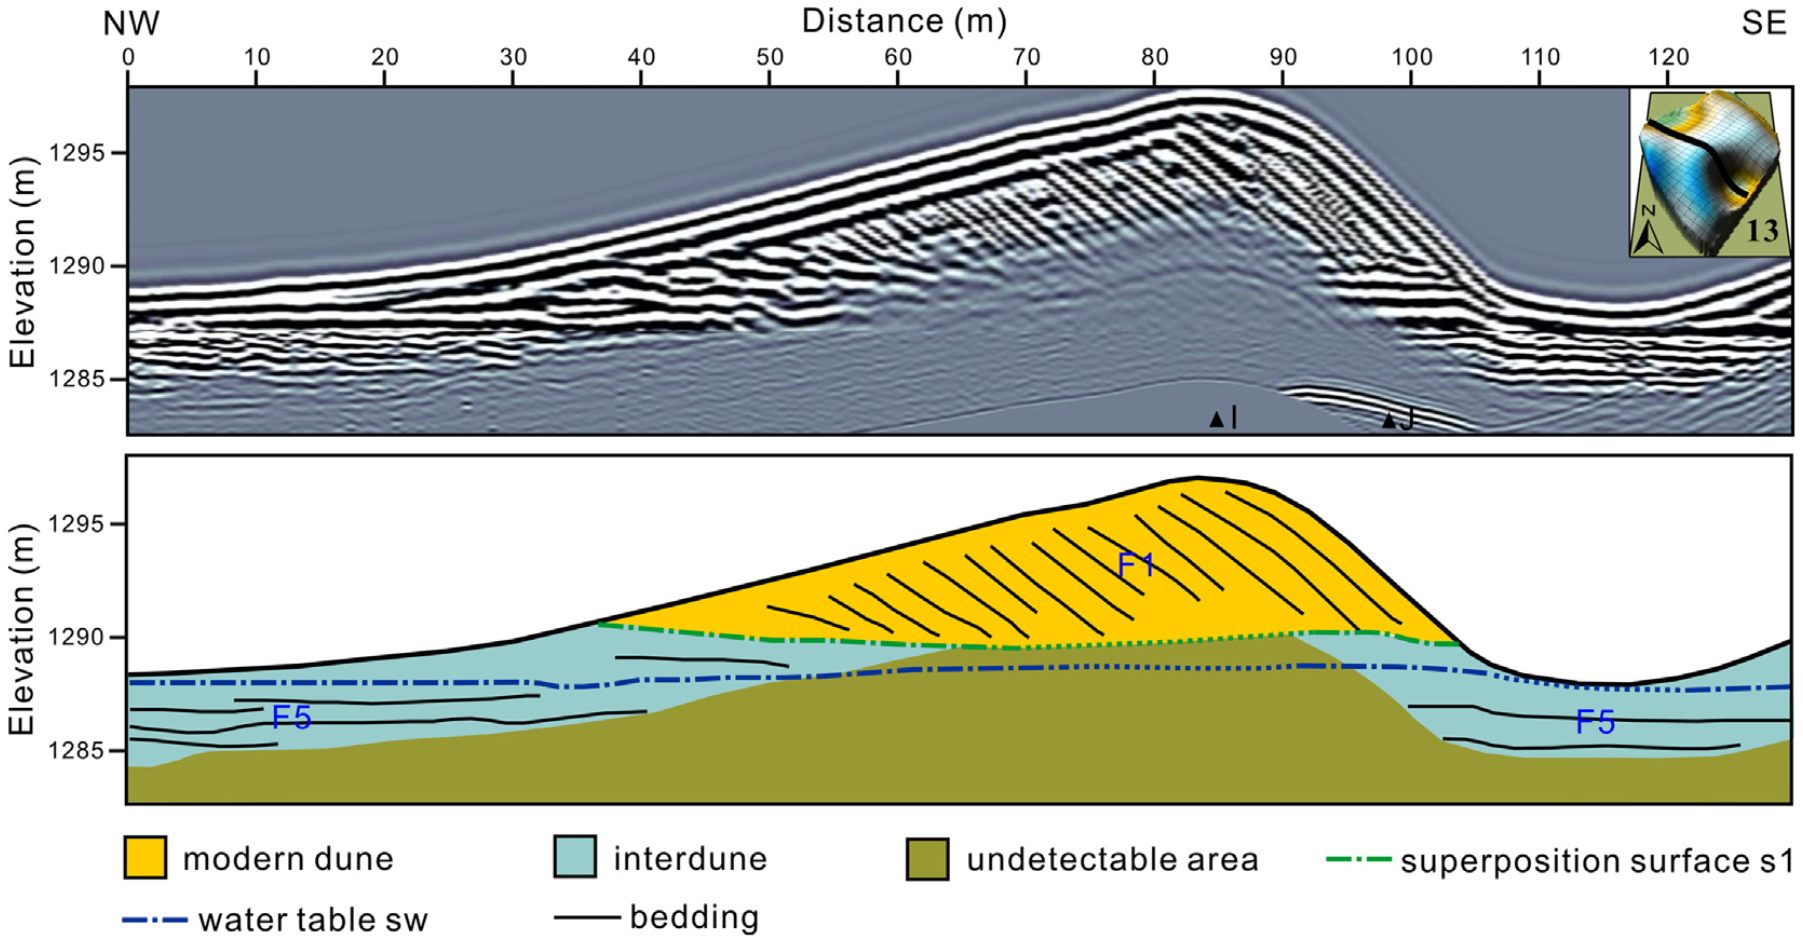
\includegraphics[width=0.9\linewidth]{Figures/0.2GPR/Fu_2019_dunes_2.png}
    \caption[Barchan dune (2).]{Barchan dune (2). \textbf{Keywords: } Horizontal, dipping, high reflectivity, low reflectivity, parallel, semi-continuous \citep{Fu2024}.}
    \label{fig:Fu2019-2}
\end{figure}

\begin{figure}[h!]
    \centering
    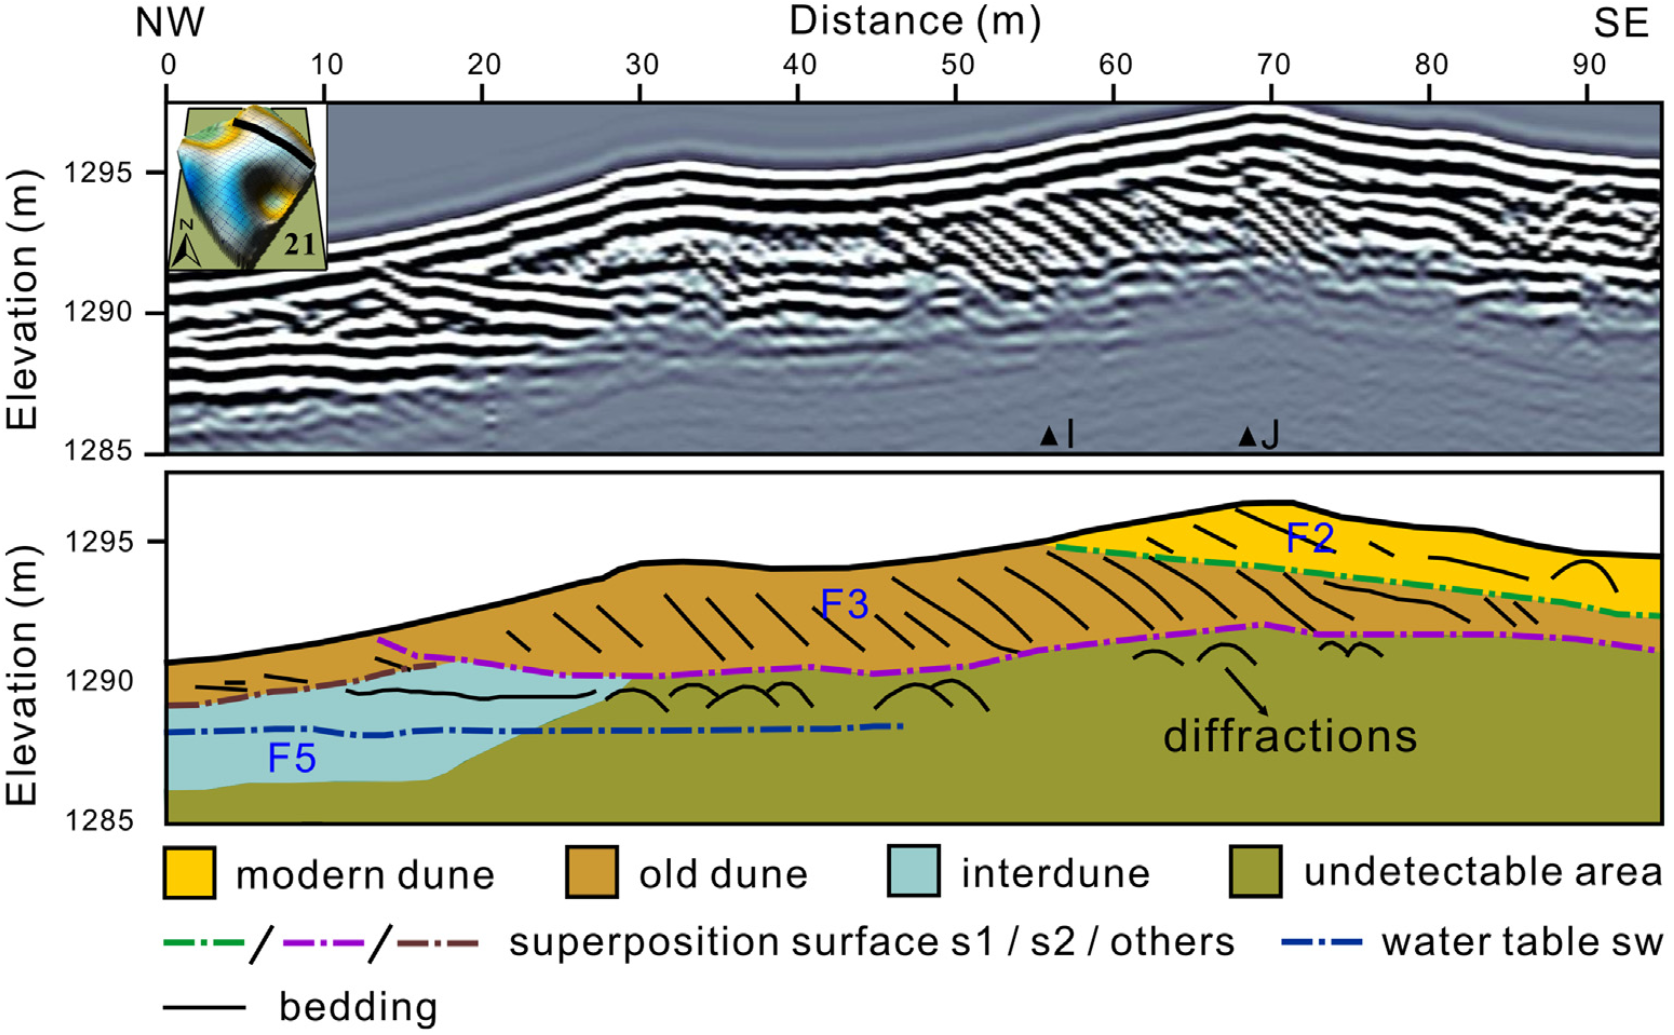
\includegraphics[width=0.9\linewidth]{Figures/0.2GPR/Fu_2019_dunes_4.png}
    \caption[Barchan dune (2).]{Barchan dune (2). \textbf{Keywords: } Parallel, semi-horizontal, semi-continuous, dipping, hummocky, diffraction hyperbola, high reflectivity, low reflectivity \citep{Fu2024}.}
    \label{fig:Fu2019-4}
\end{figure}

\begin{figure}[h!]
    \centering
    
\includegraphics[width=0.9\linewidth]{Figures/0.2GPR/VanHeteren_1998_Coastal.png}
    \caption[Paraglacial coastal setting.]{Paraglacial coastal setting. \textbf{Keywords: } Chaotic, parallel, oblique, hyperbolic, high-frequency, low-frequency, tangential, sigmoidal, hummocky, bounding surface \citep{VanHeteren1998}.}
    \label{fig:VanHeteren1998-1}
\end{figure}
\clearpage
\subsubsection{Lacustrine}
\begin{table}[h!]
\centering
\caption{Categorised GPR profile keywords for lacustrine environments. Geometry, reflectivity and continuity are shown in separate columns.}
\begin{tabular}{|p{4.5cm}|p{4.5cm}|p{4.5cm}|}
\hline
\textbf{Geometry / Structure} & \textbf{Continuity} & \textbf{Amplitude / Reflectivity} \\
\hline
Mounded & Continuous & Medium amplitude \\
Downlap & Semi-continuous & High amplitude \\
Dipping & Discontinuous & Low amplitude \\
Lenticular & Wavy & High reflectivity \\
Concave & & Low reflectivity \\
Layered & & Varied reflectivity \\
Oblique & & High attenuation \\
Wedge & & \\
Prograding & & \\
Clinoform & & \\
Sigmoidal & & \\
Horizontal & & \\
Parallel & & \\
Subparallel & & \\
Foreset truncation & & \\
Sub-horizontal & & \\
\hline
\end{tabular}
\label{tab:lacustrine-keywords}
\end{table}

\begin{figure}[h!]
    \centering
    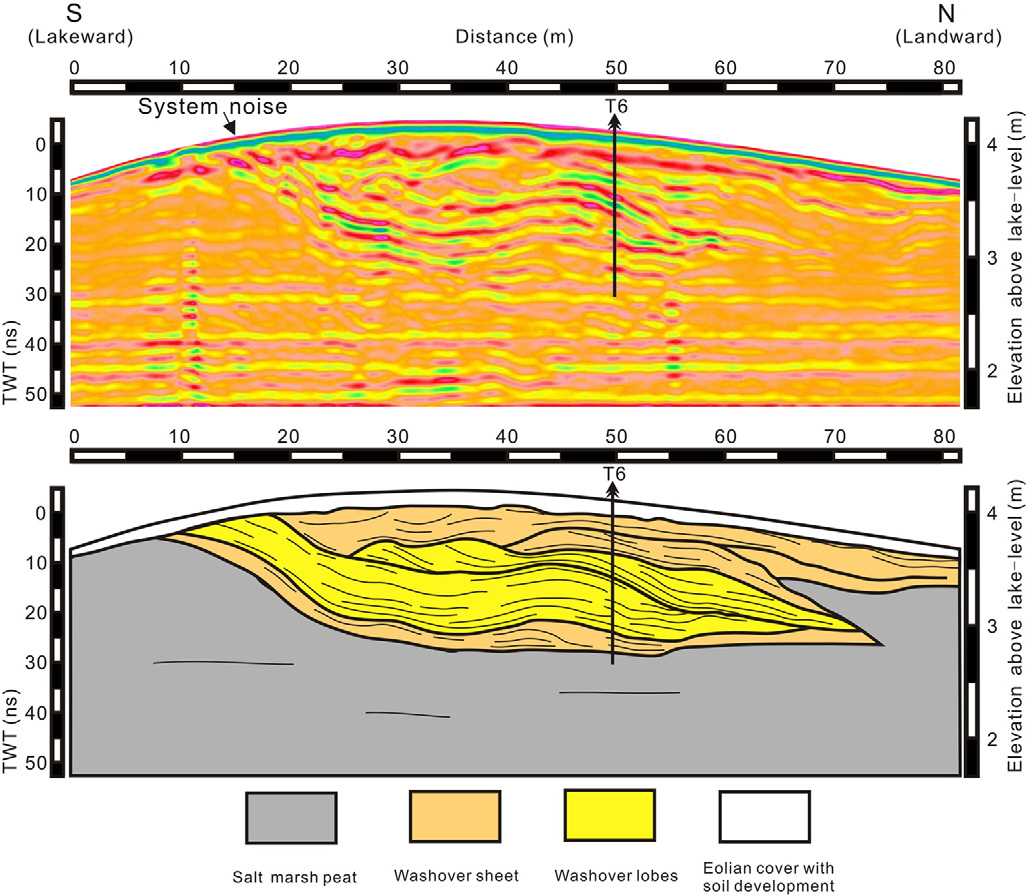
\includegraphics[width=0.9\linewidth]{Figures/0.2GPR/Shan2015_fill_3.png}
    \caption[Shore-parallel profile of trenches (1).]{Shore-parallel profile of trenches (1).\textbf{Keywords: } Mounded, downlap, dipping, lenticular, concave, layered, continuous, semi-continuous, discontinuous, medium amplitude, high amplitude, high reflectivity, low reflectivity \citep{Shan2015}.}
    \label{fig:Shan2015-3}
\end{figure}
\begin{figure}[h!]
    \centering
    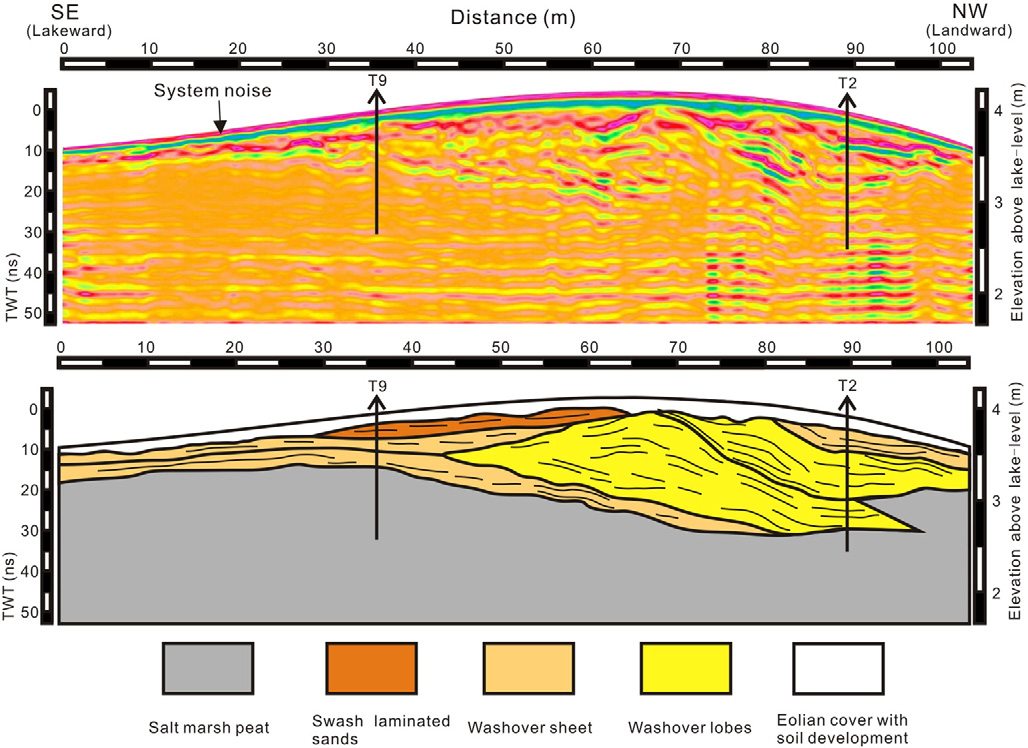
\includegraphics[width=0.9\linewidth]{Figures/0.2GPR/Shan2015_fill_4.png}
    \caption[Shore-parallel profile of trenches (2).]{Shore-parallel profile of trenches (2). \textbf{Keywords: } Oblique, wedge, concave, semi-continuous, wavy, discontinuous, high amplitude, low amplitude, varied reflectivity\citep{Shan2015}.}
    \label{fig:Shan2015-4}
\end{figure}

\begin{figure}[h!]
    \centering
    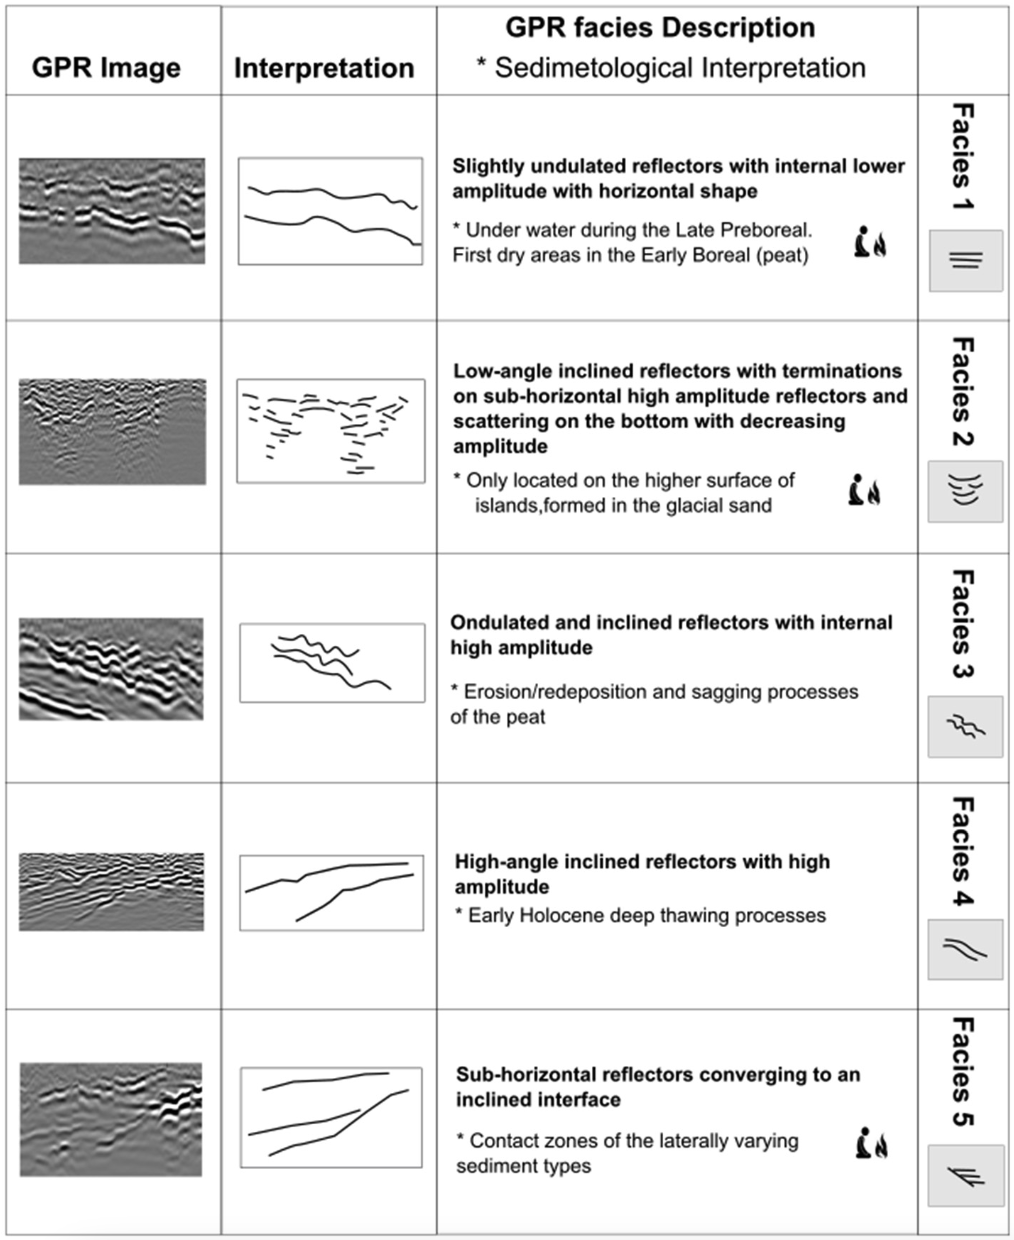
\includegraphics[width=0.9\linewidth]{Figures/0.2GPR/Corradini_2023_lake_bog.png}
    \caption[Lake and bog.]{Lake and bog. \textbf{Keywords: } Low amplitude, discontinuous, dipping, high amplitude, high attenuation, sub-horizontal \citep{Corradini2023}.}
    \label{fig:Corradini2023-1}
\end{figure}

\begin{figure}[h!]
    \centering
    \includegraphics[width=0.9\linewidth]{Figures/0.2GPR/Jol1991_1.png}
    \caption[Lacustrine delta (1).]{Lacustrine delta (1). \textbf{Keywords: } Prograding, clinoform, downlap, sigmoidal, continuous, horizontal, dipping, high attenuation \citep{Jol1991-1}.}
    \label{fig:Jol1991-1}
\end{figure}

\begin{figure}[h!]
    \centering
    \includegraphics[width=0.9\linewidth]{Figures/0.2GPR/Jol1991_2_1.png}
    \caption[Lacustrine delta (2).]{Lacustrine delta (2). \textbf{Keywords: } Clinoform, downlap, dipping, parallel, subparallel topset, continuous, prograding, foreset truncation, high attenuation \citep{Jol1991-1}.}
    \label{fig:Jol1991-2-1}
\end{figure}
\clearpage
\subsubsection{Igneous}
\begin{table}[h!]
\caption{Categorised GPR profile keywords for igneous environments. Geometry, reflectivity and continuity are shown in separate columns.}
\centering
\small
\begin{tabular}{|p{4.5cm}|p{4.5cm}|p{4.5cm}|}
\hline
\textbf{Geometry} & \textbf{Amplitude / Reflectivity} & \textbf{Continuity} \\
\hline
Concave & Alternating reflectivity & Continuous \\
Concave up structures & Attenuated & Crossing reflectors \\
Fill & High attenuation & Discontinuous \\
Scour & High reflectivity & Horizontal \\
Tangential & Low reflection & Parallel \\
Chaotic & Varied attenuation & Subparallel \\
Complex & Varied reflectivity & Semi-continuous \\
Dipping & & \\
Even & & \\
Hummocky & & \\
Hyperbolic & & \\
Irregular & & \\
Lenticular & & \\
Multidirectional dipping & & \\
Oblique & & \\
Sigmoidal & & \\
Sub-horizontal & & \\
Transparent zones & & \\
Wavy & & \\
Diffraction & & \\
Diffraction hyperbola & & \\
Horizontal layering & & \\
\hline
\end{tabular}
\label{tab:merged_gpr_keywords}
\end{table}

\begin{landscape}
\begin{figure}[h!]
    \centering
    \includegraphics[width=0.9\linewidth]{Figures/0.2GPR/Ettinger2014_lahar_7.png}
    \caption[Lahar-generated fan (1).]{Lahar-generated fan (2). \textbf{Keywords: }Irregular, wavy, discontinuous, hummocky, parallel, subparallel \citep{Ettinger2014}.}
    \label{fig:Ettinger2014-7}
\end{figure}
\end{landscape}

\begin{landscape}
    \begin{figure}[h!]
    \centering
    \includegraphics[width=0.9\linewidth]{Figures/0.2GPR/Ettinger2014_lahar_1.png}
    \caption[Lahar-generated fan (2).]{Lahar-generated fan (1). \textbf{Keywords: }Scour, fill, parallel, irregular, even, wavy, sigmoidal, subparallel, oblique, attenuated, complex, truncation, tangential, chaotic, diffraction, hummocky, discontinuous \citep{Ettinger2014}. }
    \label{fig:Ettinger2014-1}
\end{figure}
\end{landscape}
\clearpage

\begin{landscape}
    \begin{figure}[h!]
    \centering
    \includegraphics[width=0.9\linewidth]{Figures/0.2GPR/Gomez_2009_pyro.jpg}
    \caption[Pyroclastic flow.]{Pyroclastic flow. \textbf{Keywords: } Varied reflectivity, \citep{Gomez-2009-1}.}
    \label{fig:Gomez2009-1}
\end{figure}
\end{landscape}
\clearpage

\begin{figure}[h!]
    \centering
    \includegraphics[width=0.9\linewidth]{Figures/0.2GPR/Gomez2018_1.jpg}
    \caption[Lahar deposit (1).]{Lahar deposit (1). \textbf{Keywords: } Concave up structures, prograding units, chaotic, truncation, hyperbolic, discontinuous, dipping, semi-continuous, multidirectional dipping, lenticular, low reflectivity.
   \citep{Gomez2018}.}
    \label{fig:Gomez2018-1}
\end{figure}

\begin{landscape}
    \begin{figure}[h!]
    \centering
    \includegraphics[width=0.9\linewidth]{Figures/0.2GPR/Gomez2018_2.jpg}
    \caption[Lahar deposit (2).]{Lahar deposit (2). \textbf{Keywords: } Horizontal layering, parallel, transparent zones, chaotic, discontinuous, alternating reflectivity, semi-continuous, dipping, high attenuation \citep{Gomez2018}.}
    \label{fig:Gomez2018-2}
\end{figure}
\end{landscape}
\clearpage

\begin{figure}[h!]
    \centering
    \includegraphics[width=0.9\linewidth]{Figures/0.2GPR/Kruse2010_tephra_3.png}
    \caption[Irazú intracrater tephra 1963-1965 deposits.]{\textbf{Keywords: } Parallel, semi-continous, dipping, hummocky, discontinous \citep{Kruse2010}.}
    \label{fig:Kruse2010-3}
\end{figure}
\clearpage

\begin{figure}[h!]
    \centering
    \includegraphics[width=0.9\linewidth]{Figures/0.2GPR/Rust2000_pyroclast_1.png}
    \caption[Welding in pyroclastic flows pre-migration.]{Welding in pyroclastic flows. \textbf{Keywords: } Parallel, dipping, sub-horizontal, continuous, discontinuous, varied attenuation, hummocky, crossing reflectors \citep{Rust2000}.}
    \label{fig:Rust2000-1}
\end{figure}

\begin{figure}[h!]
    \centering
    \includegraphics[width=0.9\linewidth]{Figures/0.2GPR/Rust2000_pyroclast_2.png}
    \caption[Welding in pyroclastic flows post-migration.]{Welding in pyroclastic flows. \textbf{Keywords: } Sub-horizontal, varied attenuation, semi-continuous, dipping, discontinuous, hummocky \citep{Rust2000}.}
    \label{fig:Rust2000-2}
\end{figure}
\clearpage


\begin{figure}[h!]
    \centering
    \includegraphics[width=0.9\linewidth]{Figures/0.2GPR/Gertisser2009_Block_Ash_1.png}
    \caption[Overbank block-and-ash flow deposits (1).]{Overbank block-and-ash flow deposits (1). \textbf{Keywords: } Differaction hyperbola, dipping, continuous, discontinuous, chaotic, low reflection \citep{Gertisser2012}.}
    \label{fig:Gertisser2012-1}
\end{figure}
\clearpage
\begin{figure}[h!]
    \centering
    \includegraphics[width=0.9\linewidth]{Figures/0.2GPR/Gertisser2009_Block_Ash_2.png}
    \caption[Overbank block-and-ash flow deposits (2).]{Overbank block-and-ash flow deposits (2). \textbf{Keywords: } Differaction hyperbola, dipping, horizontal, semi-continuous, discontinuous, high reflectivity, continuous \citep{Gertisser2012}.}
    \label{fig:Gertisser2012-2}
\end{figure}
\clearpage

\begin{figure}[h!]
    \centering
    \includegraphics[width=0.9\linewidth]{Figures/0.2GPR/Russel1996_volcanic_deposits_1.png}
    \caption[Basalt lava flow (1).]{Basalt lava flow (1). \textbf{Keyword:} Hummocky, irregular, discontinuous, dipping, high attenuation, horizontal, crossing reflectors \citep{Russell1997}.}
    \label{fig:Russell1996-1}
\end{figure}

\begin{figure}[h!]
    \centering
    \includegraphics[width=0.9\linewidth]{Figures/0.2GPR/Russel1996_volcanic_deposits_3.png}
    \caption[Basalt lava flow (2).]{Basalt lava flow (1). \textbf{Keywords: } Dipping, high attenuation, discontinuous, horizontal, multidirectional dipping \citep{Russell1997}.}
    \label{fig:Russel2017-3}
\end{figure}

\begin{landscape}
\begin{figure}[h!]
    \centering
    \includegraphics[width=0.9\linewidth]{Figures/0.2GPR/Russel1996_volcanic_deposits_5.png}
    \caption[Pumice talus deposit.]{Pumice talus deposit. \textbf{Keywords: } Discontinuous, dipping, high attenuation, horizontal, multidirectional dipping, hummocky, concave \citep{Russell1997}.}
    \label{fig:Russell1996-5}
\end{figure}
\end{landscape}
\clearpage

\clearpage
\subsection{Seismic}
\begin{table}[h!]
\centering
\caption{Categorised seismic profile keywords based on geometry, continuity and frequency.}
\begin{tabular}{|p{4.5cm}|p{4.5cm}|p{4.5cm}|}
\hline
\textbf{Geometry / Structure} & \textbf{Continuity} & \textbf{Frequency / Amplitude} \\
\hline
Bowl & Continuous & High amplitude \\
Chaotic & Discontinuous & High frequency \\
Clinoforms & High continuity & Low amplitude \\
Concave & Low continuity & Low frequency \\
Convex & Medium continuity & Medium amplitude \\
Dipping & Moderate continuity & Medium frequency \\
Downlap & Poor continuity & Moderate amplitude \\
Draping & Semi-continuous & Varied frequency \\
Faulting & Semi-chaotic & \\
Horizontal & & \\
Hyperbolic & & \\
Inclined & & \\
Incision & & \\
Lateral & & \\
Onlap & & \\
Lenticular & & \\
Linear & & \\
Mounded & & \\
Oblique & & \\
Planar & & \\
Prograding & & \\
Parallel & & \\
Semi-parallel & & \\
Shingled & & \\
Sheeted & & \\
Sigmoidal & & \\
Sloping & & \\
Progradation/aggradation & & \\
Tabular & & \\
Tangential & & \\
Toplap & & \\
Truncation & & \\
U-shaped & & \\
Undulate & & \\
Wavy & & \\
Subparallel & & \\
\hline
\end{tabular}
\label{tab:separated_keywords}
\end{table}

\subsubsection{Marine}
\begin{figure}[ht!]
    \centering
    \includegraphics[width=0.9\linewidth]{Figures/0.2GPR/Kaci2024_shelf.png}
    \caption[Structural history of inner shelf.]{Structural history of inner shelf. \textbf{Keywords:}Low continuity, high continuity, oblique, subparallel, sigmoidal, prograding, onlap, downlap, parallel aggrading, toplap, chaotic, concave, convex, divergent, dipping \citep{Kaci2024}.}
    \label{fig:Kaci2024-1}
\end{figure}

\begin{figure}[h!]
    \centering
    \includegraphics[width=0.9\linewidth]{Figures/0.3Seismic/Pellegrini2018-1.jpg}
    \caption[River lowstand wedge.]{River lowstand wedge. \textbf{Keywords: }High amplitude, low amplitude, continuous, chaotic, discontinuous, dipping, wavy, hyperbolic, semi-continuous, mounded \citep{Pellegrini2018}.}
    \label{fig:Pellegrini2018-1}
\end{figure}

\begin{figure}[h!]
    \centering
    \includegraphics[width=0.9\linewidth]{Figures/0.3Seismic/Thieblemont2020-1.jpg}
    \caption[Channel systems (1).]{Channel systems (1). \textbf{Keywords: }Sigmoidal, oblique, low amplitude, high amplitude, discontinuous, horizontal, continuous, parallel, subparallel, moderate amplitude, lenticular, chaotic, convex, bowl \citep{Thieblemont2020}.}
    \label{fig:Thieblemont2020-1}
\end{figure}

\begin{figure}[h!]
    \centering
    \includegraphics[width=0.9\linewidth]{Figures/0.3Seismic/Thieblemont2020-2.jpg}
    \caption[Channel systems (2)]{Channel systems (2). \textbf{Keywords: }Low amplitude, parallel, tangential, oblique, mounded, high amplitude, discontinuous, continuous, subparallel, chaotic, u-shaped, sheeted, dipping, wavy, moderate amplitude, tabular, bowl, linear \citep{Thieblemont2020}.}
    \label{fig:Thieblemont2020-2}
\end{figure}
\clearpage

\begin{figure}[h!]
    \centering
    \includegraphics[width=0.75\linewidth]{Figures/0.3Seismic/Thieblemont2020-3.jpg}
    \caption[Channel systems (3).]{Channel systems (3). \textbf{Keywords: } Wavy, dipping, draping, parallel \citep{Thieblemont2020}.}
    \label{fig:Thieblemont2020-3}
\end{figure}

\begin{figure}[h!]
    \centering
    \includegraphics[width=0.75\linewidth]{Figures/0.3Seismic/Andrade2018_trace_1.png}
    \caption[Marginal ridge development.]{Marginal ridge development. \textbf{Keywords: } Parallel, wavy, high amplitude, low amplitude, medium amplitude, planar, semi-parallel, prograding, dipping, inclined, discontinuous, subparallel, chaotic, undulate, faulting, semi-chaotic \citep{Andrade2018}.}
    \label{fig:Andrade2018-1}
\end{figure}

\begin{figure}[h!]
    \centering
    \includegraphics[width=0.9\linewidth]{Figures/0.3Seismic/Winata2023-1.jpg}
    \caption[Passive margin sequences.]{Passive margin sequences. \textbf{Keywords: } Medium amplitude, high amplitude, parallel, lateral, continuous, low amplitude, subparallel, semi-continuous, faulting, wavy, discontinuous, chaotic, incision, stacked progradation/aggradation \citep{winata2023}.}
    \label{fig:Winata2023-1}
\end{figure}

\begin{figure}[h!]
    \centering
    \includegraphics[width=0.9\linewidth]{Figures/0.3Seismic/Bourget2014_trace_1.png}
    \caption[Tide and wave dominated shelf-edge delta.]{Tide and wave dominated shelf-edge delta. \textbf{Keywords: } Oblique, sigmoidal, prograding/aggrading prodelta, sloping, dipping, low amplitude, medium amplitude, parallel, clinoforms, prograding, lateral progredation, onlap, chaotic, horizontal \citep{Bourget2014}.}
    \label{fig:Bourget2014-1}
\end{figure}

\begin{figure}[h!]
    \centering
    \includegraphics[width=0.9\linewidth]{Figures/0.3Seismic/Calves2019_trace_1.png}
    \caption[Basin fluvial system.]{Basin fluvial system. \textbf{Keywords: } High amplitude, moderate amplitude, continuous, low amplitude, moderate continuity, shingled \citep{Calves2019}.}
    \label{fig:Calves2019-1}
\end{figure}

\begin{figure}[h!]
    \centering
    \includegraphics[width=0.9\linewidth]{Figures/0.3Seismic/Chen2017_River_trace_1.png}
    \caption[Eocene sedimentation.]{Eocene sedimentation. \textbf{Keywords: } Low frequency, medium frequency, low amplitude, medium amplitude, high amplitude, poor continuity, medium continuity, low continuity, subparallel, chaotic, parallel, dipping, horizontal \citep{Chen2017}.}
    \label{fig:Chen2017-1}
\end{figure}

\begin{figure}[h!]
    \centering
    \includegraphics[width=0.75\linewidth]{Figures/0.3Seismic/Chima2019_Basin_trace_1.png}
    \caption[Offshore delta.]{Offshore delta. \textbf{Keywords: } High amplitude, medium amplitude, low amplitude, discontinuous, continuous, horizontal, dipping,  sub-parallel \citep{Chima2019}.}
    \label{fig:Chima2019-1}
\end{figure}

\begin{figure}[h!]
    \centering
    \includegraphics[width=0.9\linewidth]{Figures/0.3Seismic/Ding2014_Carbonates_trace_1.png}
    \caption[Tectono-sedimentary evolution (1).]{Tectono-sedimentary evolution (1). \textbf{Keywords: } Parallel, wavy, subparallel, chaotic, varied frequency, high continuity, low continuity, medium continuity, high amplitude, medium amplitude, low amplitude \citep{Ding2015}.}
    \label{fig:Ding2015-1}
\end{figure}

\begin{figure}[h!]
    \centering
    \includegraphics[width=0.9\linewidth]{Figures/0.3Seismic/Ding2014_Carbonates_trace_2.png}
    \caption[Tectono-sedimentary evolution (2).]{Tectono-sedimentary evolution (2). \textbf{Keywords: } Parallel, subparallel, high amplitude, medium amplitude, high continuity, medium continuity, truncation  \citep{Ding2015}.}
    \label{fig:Ding2015-2}
\end{figure}

\begin{figure}[h!]
    \centering
    \includegraphics[width=0.9\linewidth]{Figures/0.3Seismic/Deng2017_buriedhill.png}
    \caption[Buried hill]{\textbf{Keywords: } Low amplitude, poor continuity, low frequency, medium amplitude, medium continuity, parallel, dipping, high amplitude, high continuity, chaotic, lateral slope, wavy \citep{Deng2017}.}
    \label{fig:Deng2017-1}
\end{figure}
\clearpage

\begin{figure}[h!]
    \centering
    \includegraphics[width=0.9\linewidth]{Figures/0.3Seismic/Escobar2024_delta.png}
    \caption[Transform fault river delta.]{Transform fault river delta. \textbf{Keywords:} Parallel, divergent, continuous, medium amplitude, high amplitude, high frequency, chaotic, low amplitude, semi-continuous, low frequency, medium frequency \citep{Escobar2024}.}
    \label{fig:Escobar2024-1}
\end{figure}

%\begin{figure}[h!]
%    \centering
%    \includegraphics[width=0.75\linewidth]{Figures/0.3Seismic/kalani2020.jpg}
%    \caption[]{\textbf{Keywords: } \citep{Kalani2020}.}
%    \label{fig:Kalani2020}
%\end{figure}
%\clearpage
%\begin{figure}[h!]
%    \centering
%    \includegraphics[width=0.75\linewidth]{Figures/0.3Seismic/Barrera2021.jpg}
%    \caption[]{\textbf{Keywords: } \citep{Barrera2021}.}
%    \label{fig:Barrera2021}
%\end{figure}
\clearpage
\subsection{Field Observations}
This section contains outcrop data of a few selected field areas. 
\begin{table}[h!]
\centering
\caption{Unique sedimentary interpretation keywords extracted from field analogue studies.}
\begin{tabular}{|p{4cm}|p{4cm}|p{4cm}|}
\hline
\multicolumn{3}{|c|}{\textbf{Geometries / structures}} \\
\hline
Chaotic bedding & Concave & Continuous \\
Cross-stratification & Deformation & Dipping \\
Discontinuous & Erosion & Cross-bedding \\
Fill deposit & Fine/coarse-grained & Horizontal \\
Horizontal bedding & Irregular & Laminate \\
Laterally stacked & Lenticular & onlap \\
Low angle & Parallel & Planar \\
Ripples & Semi-continuous & Shallow scours \\
Sinuous & Sinusoidal stratification & Tabular \\
Trace fossils & Vertically stacked & Wavy pattern \\
\hline
\end{tabular}
\label{tab:field-keywords}
\end{table}

\subsubsection{Lacustrine}
\begin{figure}[h!]
    \centering
    \includegraphics[width=0.75\linewidth]{Figures/0.4Field/Cui2023_trace_field_1.png}
    \caption[Siliciclastic-carbonate lacustrine system]{Siliciclastic-carbonate lacustrine system \citep{Cui2023}. \textbf{Keywords:} low-angle wedge, cross-stratification, planar lamination, parallel, wavy pattern, chaotic bedding, deformation}
    \label{fig:Cui23-1}
\end{figure}
\clearpage

\subsubsection{Fluvial}
\begin{figure}[h!]
    \centering
    \includegraphics[width=0.75\linewidth]{Figures/0.4Field/Alvan2018_trace_field_1.png}
    \caption[An overview of several Sedimenatry facies]{An overview of several Sedimenatry facies\citep{Alvan2018}. \textbf{Keywords:} Cross lamination, fill deposit, coarse-grained, fine-grained, parallel, lenticular, horizontal layers.}
    \label{fig:Alvan2018-1}
\end{figure}

\begin{figure}[h!]
    \centering
    \includegraphics[width=0.75\linewidth]{Figures/0.4Field/Alvan2018_trace_field_2.png}
    \caption[An overview of several Sedimenatry facies]{An overview of several Sedimenatry facies\citep{Alvan2018}. \textbf{Keywords:} Lateral extension, parallel, onlap, downlap, sinuous, cross-bedding.}
    \label{fig:Alvan2018-2}
\end{figure}

\begin{figure}[h!]
    \centering
    \includegraphics[width=0.75\linewidth]{Figures/0.4Field/Winsemann2022.png}
    \caption[Characteristics of channel bodies and sheetflood deposits]{Characteristics of channel bodies and sheetflood deposits \citep{Winsemann2022}. \textbf{Keywords:} Concave, laterally stacked, vertically stacked, erosional surface, dipping, cross-stratification, sinusoidal stratification, low angle, ripple.}
    \label{fig:Winsemann22-1}
\end{figure}

\begin{figure}[h!]
    \centering
    \includegraphics[width=0.75\linewidth]{Figures/0.4Field/Poursoltani2020.png}
    \caption[Summary of architectural elements in a lower sandstone]{Summary of architectural elements in a lower sandstone \citep{Poursoltani2020}. \textbf{Keywords:} Laterally extensive, erosional surface, irregular, concave-up, cross-bedding, horizontal, dipping.}
    \label{fig:Poursoltani20-1}
\end{figure}

\begin{figure}[h!]
    \centering
    \includegraphics[width=0.75\linewidth]{Figures/0.4Field/Guo2022_2.png}
    \caption[Channel architecture of the outcrop section of the Yungang Formation (1)]{Channel architecture of the outcrop section of the Yungang Formation \citep{Guo2022}. \textbf{Keywords:} Cross-bedding, dipping, onlap, erosion.}
    \label{fig:Guo2022-2}
\end{figure}

\begin{figure}[h!]
    \centering
    \includegraphics[width=0.75\linewidth]{Figures/0.4Field/Guo2022_3.png}
    \caption[Channel architecture of the outcrop section of the Yungang Formation (2)]{Channel architecture of the outcrop section of the Yungang Formation \citep{Guo2022}. \textbf{Keywords:} Cross-bedding, erosion, dipping, onlap.}
    \label{fig:Guo2022-3}
\end{figure}
\begin{figure}[h!]
    \centering
    \includegraphics[width=0.75\linewidth]{Figures/0.4Field/Guo2022_4.png}
    \caption[Channel architecture of the outcrop section of the Yungang Formation (3)]{Channel architecture of the outcrop section of the Yungang Formation \citep{Guo2022}. \textbf{Keywords:} Cross-bedding, erosion, dipping, onlap, horizontal layering, semi-continuous, continuous.}
    \label{fig:Guo2022-4}
\end{figure}

\begin{figure}[h!]
    \centering
    \includegraphics[width=0.75\linewidth]{Figures/0.4Field/Paz2022.jpg}
    \caption[Contourite drift facies]{Contourite drift facies \citep{Paz2022}. \textbf{Keywords:} Discontinuous, continuous, planar, parallel, low-angle, wavy pattern, lenticular shape, cross-bedding, erosional surface, tabular, cross-lamination.}
    \label{fig:Paz2022-1}
\end{figure}

\begin{figure}[h!]
    \centering
    \includegraphics[width=0.75\linewidth]{Figures/0.4Field/Capuzzo2004-1.png}
    \caption[Facies description and classification in the Salvan-Dorénaz Basin]{Facies description and classification in the Salvan-Dorénaz Basin \citep{Capuzzo2004}.\textbf{Keywords:} Horizontal bedding, cross-stratification, planar, tabular, shallow scours, ripples, lamination.}
    \label{fig:Capuzzo2004-1}
\end{figure}
\clearpage
\clearpage
\section{Mars}
\subsection{RIMFAX}
This chapter contains published interpretations done on RIMFAX data, with the latest update of the chapter being done in May 2025. 

\begin{table}[h!]
\centering
\caption{Grouped radar interpretation keywords extracted from the RIMFAX dataset.}
\begin{tabular}{|p{6.8cm}|p{6.8cm}|}
\hline
\textbf{Geometry / Structure} & \textbf{Geometry / Structure (cont.)} \\
\hline
Bumpy & Ridge \\
Clinoform structures & Semi-horizontal layering \\
Concave up structures & Sub-horizontal \\
Crossing reflectors & Sigmoidal profiles \\
Dipping & Sloped-surface \\
Horizontal layering & Sloping reflectors \\
Hummocky & Subparallel \\
Lenticular reflectors & Transparent unit \\
Onlap & Multidirectional dipping \\
\hline
\textbf{Amplitude / Reflectivity} & \textbf{Continuity} \\
\hline
Attenuated signal & Coherent near-surface layering \\
High reflectivity & Continuous \\
Low reflectivity & Discontinuous layers \\
Strong reflectivity & Low continuity \\
Strong surface reflections & Semi-continuous \\
Weak reflectivity & Sparse internal reflections \\
Transparent zones & \\
\hline
\textbf{Terminations / Surfaces} & \textbf{Other / Descriptive} \\
\hline
Erosional contact & Chaotic \\
Truncating reflections & Parallel \\
Truncation & \\
\hline
\end{tabular}
\label{tab:rimfax-keywords}
\end{table}

\clearpage
\subsubsection{Igneous}
The article by \citet{Hamran2022} does not strictly conclude with a specific depositional environment. However, it does lean more towards an igneous explanation, thus placing the interpretations in this section. Furthermore, within the igneous hypothesis is the suggestion of the layered intrusions. There are no terrestrial GPR analogues for this structure yet, however, some of the structures within this section are interpreted as layered intrusions. 
\begin{figure}[h!]
    \centering
    \includegraphics[width=0.9\linewidth]{Figures/0.5RIMFAX/Hamran_2022-f3.jpg}
    \caption[RIMFAX transition between two packages from sol 278 to 286]{RIMFAX transition between two packages from sol 278 to 286 \citep{Hamran2022}. \textbf{Keywords:} Strongly dipping reflectors, truncating reflections, clinoform structures, continuous to discontinuous, high to low reflectivity.}
    \label{fig:Hamran22-3}
\end{figure}

\begin{figure}[h!]
    \centering
    \includegraphics[width=0.9\linewidth]{Figures/0.5RIMFAX/Hamran_2022-f4.jpg}
    \caption[RIMFAX radargram acquired from Sol 201 and Sol 202.]{RIMFAX radargram acquired from Sol 201 and Sol 202 \citep{Hamran2022}. \textbf{Keywords:} Attenuated signal, radar-transparent zones, sparse internal reflections, dipping layers, semi-layered, multidirectional dipping, discontinuous layers, semi-continuous layers.}
    \label{fig:Hamran22-4}
\end{figure}

\begin{figure}
    \centering
    \includegraphics[width=0.9\linewidth]{Figures/0.5RIMFAX/Hamran_2022-f5.jpg}
    \caption[RIMFAX radar facies observed during Sol 201 and Sol 202.]{RIMFAX radar facies observed during Sol 201 and Sol 202 \citep{Hamran2022}. \textbf{Keywords:} Coherent near-surface layering, subparallel, low reflectivity, high reflectivity, dipping layers, parallel, sub-horizontal, lenticular reflectors, sigmoidal profiles.}
    \label{fig:Hamran22-5}
\end{figure}

\clearpage

\begin{figure}[h!]
    \centering
    \includegraphics[width=0.9\linewidth]{Figures/0.5RIMFAX/Horgan_2023-fig1.jpg}
    \caption[RIMFAX traverse from sol 112–123.]{RIMFAX traverse from sol 112–123 \citep{Horgan2023}. \textbf{Keywords:} Strong surface reflections, transparent unit, low-density fill, low reflectivity, chaotic.}
    \label{fig:Horgan23-1}
\end{figure}

\begin{figure}[h!]
    \centering
    \includegraphics[width=0.9\linewidth]{Figures/0.5RIMFAX/Simon_2023-fig-03.jpg}
    \caption[RIMFAX traverse from sol 210]{RIMFAX traverse from sol 210 \citep{Simon2023}. \textbf{Keywords: } Sloped-surface, discontinuous, dipping, lenticulars.}
    \label{fig:Simon23-3}
\end{figure}
 
\begin{figure}[h!]
    \centering
    \includegraphics[width=0.9\linewidth]{Figures/0.5RIMFAX/Simon_2023-fig-04.jpg}
    \caption[RIMFAX Sol 200.]{RIMFAX Sol 200 \citep{Simon2023}. \textbf{Keywords:} Multi-directional dipping, semi-continuous, low continuity, ridge.}
    \label{fig:Simon23-4}
\end{figure}

\begin{figure}[h!]
    \centering
    \includegraphics[width=0.9\linewidth]{Figures/0.5RIMFAX/Simon_2023-fig-05.jpg}
    \caption[RIMFAX traverse from sol 156]{RIMFAX traverse from sol 156 \citep{Simon2023}. \textbf{Keywords:}Semi-horizontal, hummocky, lenticulars, crossing reflectors, semi-continuous, low reflectivity, high reflectivity, multi-directional dipping. }
    \label{fig:Simon23-5}
\end{figure}

\begin{figure}[h!]
    \centering
    \includegraphics[width=0.9\linewidth]{Figures/0.5RIMFAX/Simon_2023-fig-06.jpg}
    \caption[RIMFAX traverse from sol 177.]{RIMFAX traverse from sol 177 \citep{Simon2023}. \textbf{Keywords:} Dipping reflectors, semi-continuous, multi-directional dipping, low reflectivity.}
    \label{fig:Simon23-6}
\end{figure}

\begin{figure}[h!]
    \centering
    \includegraphics[width=0.9\linewidth]{Figures/0.5RIMFAX/Simon_2023-fig-07.jpg}
    \caption[RIMFAX traverse from sol 262.]{RIMFAX traverse from sol 262 \citep{Simon2023}. \textbf{Keywords:} Multi-directional dipping, low continuity, hummocky, lenticulars, horizontal layers.}
    \label{fig:Simon23-7}
\end{figure}
\clearpage
\begin{figure}[h!]
    \centering
    \includegraphics[width=0.9\linewidth]{Figures/0.5RIMFAX/Shoemaker_2024-f4.jpg}
    \caption[RIMFAX traverse from sols 383, 386, 387, and 398.]{RIMFAX traverse from sols 383, 386, 387, and 398 \citep{shoemaker2024}. \textbf{Keywords:} Sloping reflectors, parallel, low reflectivity, horizontal layering, multidirectional dipping.}
    \label{fig:Shoemaker24-4}
\end{figure}

\begin{figure}[h!]
    \centering
    \includegraphics[width=0.9\linewidth]{Figures/0.5RIMFAX/Shoemaker_2024-f5.jpg}
    \caption[RIMFAX radargram from sol 384]{RIMFAX radargram from sol 384 \citep{shoemaker2024}. \textbf{Keywords:} Truncation, high reflectivity, low reflectivity, dipping reflectors, semi-continuous, sloping reflectors.}
    \label{fig:Shoemaker24-5}
\end{figure}

\begin{figure}[h!]
    \centering
    \includegraphics[width=0.9\linewidth]{Figures/0.5RIMFAX/Shoemaker_2024-f8.jpg}
    \caption[RIMFAX radargram from sol 387.]{RIMFAX radargram from sol 387 \citep{shoemaker2024}. \textbf{Keywords:} Sloping reflectors, semi-continuous layering, parallel, semi-horizontal layering, low reflectivity, high reflectivity.}
    \label{fig:Shoemaker24-8}
\end{figure}

\begin{figure}[h!]
    \centering
    \includegraphics[width=0.9\linewidth]{Figures/0.5RIMFAX/Shoemaker_2024-f10.jpg}
    \caption[RIMFAX traverse from sol 389]{RIMFAX traverse from sol 389 \citep{shoemaker2024}. \textbf{Keywords:} Parallel, high reflectivity, low reflectivity, semi-continuous, sloping reflectors.}
    \label{fig:Shoemaker24-10}
\end{figure}

\begin{figure}[h!]
    \centering
    \includegraphics[width=0.9\linewidth]{Figures/0.5RIMFAX/Shoemaker_2024-f12.jpg}
    \caption[RIMFAX traverse sol 398.]{RIMFAX traverse sol 398 \citep{shoemaker2024}.\textbf{Keywords:} Parallel, high reflectivity, low reflectivity, dipping reflectors, semi-continuous, sloping reflectors.}
    \label{fig:Shoemaker24-12}
\end{figure}

\begin{figure}[h!]
    \centering
    \includegraphics[width=0.9\linewidth]{Figures/0.5RIMFAX/Shoemaker_2024-f16.jpg}
    \caption[RIMFAX radargrams images on sols 384, 387, 389, and 398.]{RIMFAX radargrams images on sols 384, 387, 389, and 398 \citep{shoemaker2024}. \textbf{Keywords:} Horizontal layering, dipping reflectors, multi-directional dipping.} 
    \label{fig:Shoemaker24-16}
\end{figure}
\clearpage
\subsubsection{Lacustrine delta deposits}
\begin{figure}[h!]
    \centering
    \includegraphics[width=0.9\linewidth]{Figures/0.5RIMFAX/Paige_2024-f3.jpg}
    \caption[RIMFAX traverse from sol 538–539]{RIMFAX traverse from sol 538–539 \citep{Paige2024}. \textbf{Keywords:} Erosional contact, multi-directional dipping, semi-continuous layers, high reflectivity, low reflectivity.}
    \label{fig:Paige24-3}
\end{figure}

\begin{figure}[h!]
    \centering
    \includegraphics[width=0.9\linewidth]{Figures/0.5RIMFAX/Paige_2024-f4.jpg}
    \caption[RIMFAX observed contact between the crater floor and the delta at Cape Nukshak. Sol 420–422]{RIMFAX observed contact between the crater floor and the delta at Cape Nukshak. Sol 420–422 \citep{Paige2024}.\textbf{ Keywords:} Erosional contact, multi-directional dipping, semi-continuous layers, high reflectivity, low reflectivity.}
    \label{fig:Paige24-4}
\end{figure}

\begin{figure}[h!]
    \centering
    \includegraphics[width=0.9\linewidth]{Figures/0.5RIMFAX/Paige_2024-f5.jpg}
    \caption[RIMFAX radargram from sol 641]{RIMFAX radargram at Cape Nukshak from sol 641 \citep{Paige2024}. \textbf{Keywords:} Bumpy, strong reflectivity, weak reføectivity, multi-directional dipping.}
    \label{fig:Paige24-5}
\end{figure}

\begin{figure}[h!]
    \centering
    \includegraphics[width=0.9\linewidth]{Figures/0.5RIMFAX/Stack_2024-04.jpg}
    \caption[RIMFAX radargram from sols 629, 632, and 641.]{RIMFAX radargram from sols 629, 632, and 641. \textbf{Keywords:} horizontal strata, erosional contact, onlap, dipping, concave up structures, continuous, semi-continuous, low reflectivity, high-reflectivity.}
    \label{fig:Stack24-4}
\end{figure}

\begin{figure}[h!]
    \centering
    \includegraphics[width=0.9\linewidth]{Figures/0.5RIMFAX/Stack_2024-05.jpg}
    \caption[RIMFAX radargram from sols 535, 536, 537, and 538.]{RIMFAX radargram from sols 535, 536, 537, and 538  \citep{Stack2024}. \textbf{Keywords:} Dipping, horizontal strata, continuous, semi-continuous, low reflectivity, high-reflectivity.}
    \label{fig:Stack24-5}
\end{figure}
\clearpage
\subsection{RoPeR}
This chapter contains published interpretations of RoPeR data, with the latest update being May 2025. The purpose of this section is to look into GPR data from Mars, gathered by an instrument other than RIMFAX. 

\begin{table}[h!]
\centering
\caption{Grouped radar interpretation keywords extracted from the RoPeR dataset.}
\begin{tabular}{|p{6.8cm}|p{6.8cm}|}
\hline
\textbf{Geometry / Structure} & \textbf{Geometry / Structure (cont.)} \\
\hline
Dipping reflectors & Foreshore progradation \\
Domes & Matrix/clast layers \\
Hyperbolic reflections (point scattering) & Multidirectional dipping \\
Unidirectional dip & Parallel \\
Smooth interfaces & \\
\hline
\textbf{Amplitude / Reflectivity} & \textbf{Continuity} \\
\hline
High amplitude & Continuous reflectivity\\
Low frequency & Discontinuous reflections \\
Low reflectivity & Semi-continuous \\
Varied reflectivity\\
Strong reflectivity\\
\hline
\textbf{Terminations / Surfaces} & \textbf{Other / Descriptive} \\
\hline
Fining-upwards & Chaotic reflectors \\
Multilayered & \\
\hline
\end{tabular}
\label{tab:roper-keywords}
\end{table}

\subsubsection{Flood deposits}
\begin{figure}[h!]
    \centering
    \includegraphics[width=0.9\linewidth]{Figures/0.6RoPeR/Li2022_1.png}
    \caption[Episodic hydraulic flooding sedimentation]{Episodic hydraulic flooding sedimentation \citep{Li2022}. \textbf{Keywords:} low-frequency, multi-layered, fining-upwards, Matrix/clast layers, discontinuous reflections, smooth interfaces. Weak to strong radar reflections with depth. Chaotic reflectors, multi-directional dipping.}
    \label{fig:Li2022-1}
\end{figure}
\clearpage
\subsubsection{Beach Ridge}
\begin{figure}[h!]
    \centering
    \includegraphics[width=0.9\linewidth]{Figures/0.6RoPeR/Li2025_1_3.png}
    \caption[Beach ridge deposits]{Beach ridge deposits, modified from \citep{Li2025}. \textbf{Keywords:} Dipping reflectors, unidirectional dip, multilayered, parallel, continuous reflectors, foreshore progradation, domes, hyperbolic reflections (point scattering).}
    \label{fig:Li2025-1-3}
\end{figure}

\begin{figure}[h!]
    \centering
    \includegraphics[width=0.9\linewidth]{Figures/0.6RoPeR/Li2025_2.png}
    \caption[Comparisons with Earth analogues to beach ridges]{Comparisons with Earth analogues to beach ridges \citep{Li2025}. \textbf{Keywords:} Unidirectional dipping, parallel, continuous, semi-continuous, sections of low-reflectivity, sections of strong reflectivity, multidirectional dipping.}
    \label{fig:Li2025-2}
\end{figure}

\newpage
\input{References/Sources}
\end{document}
